%%
%% cap3.tex
%% 
%% Made by Carlos Calcaneo Roldan
%% Login   <calcaneo@jogrant>
%% 
%% Started on  Mon Jul 22 15:03:25 2019 Carlos Calcaneo Roldan
%% Last update Time-stamp: <2020-jul-29.miércoles 19:05:05 ()>
%%
%%%%%%%%EL TExto Comienza abajo de aquí! 
\chapter{Halos de Materia Oscura}
\setcounter{equation}{0}

\noindent Con la intención de conocer y diferenciar diferentes cosmologías, en nuestro estudio de los halos, optamos por realizar una variedad de simulaciones de materia oscura. Desde simulaciones con cosmologías de Universos planos ($\Omega = 1$), asi como cosmologías  de universos con densidades sub-criticas ($\Omega < 1$) y super-criticas ($\Omega > 1$). Las simulaciones que realizamos {\blues tienen $16,777,216$ partículas en una caja de $50$ Mpc y se} empezaron en un corrimiento al rojo de $z=63$ hasta un $z=0$ {\blues con un numero mínimo de partículas para los grupos (DesLinkNgb) de 20. Los parámetros específicos se referencian en la tabla \ref{tab:Resumen_Sim}.}

{\blues 
\begin{table}[H]

    \begin{tabular}{|c|c|c|}

    \hline
    $\Omega$ & $\Omega_0$ & $\Omega_\lambda$ \\ \hline
    \multirow{3}{*}{$\Omega = 1$} & 0.309 & 0.691 \\ \cline{2-3} 
     & 0.691 & 0.309 \\ \cline{2-3} 
     & 0.500 & 0.500 \\ \hline
    \multirow{3}{*}{$\Omega < 1$} & 0.309 & 0.000 \\ \cline{2-3} 
     & 0.1545 & 0.691 \\ \cline{2-3} 
     & 0.309 & 0.3455 \\ \hline
    \multirow{2}{*}{$\Omega > 1$} & 0.409 & 0.691 \\ \cline{2-3} 
     & 0.309 & 0.791 \\ \hline
    \end{tabular}
    
    \caption{Se muestra un resumen de las simulaciones que se realizaron y cuales parámetros se usaron para correr GADGET-4. Son Simulaciones que corren de un redshift $z=63$ a $z=0$ con $16,777,216$ en una caja de 50 Mpc.}
    
    \label{tab:Resumen_Sim}

\end{table} 
}
%====================================================================================================================
%======================================  COSMO PLANA  ===============================================================
%====================================================================================================================
\section[Cosmología Plana \texorpdfstring{$\Omega = 1$}{Omega = 1}]{Cosmología Plana \texorpdfstring{$\Omega = 1$}{Omega = 1}}

\noindent Comenzaremos con un estudio de las cosmologías planas (aquellas donde las densidades sean $\Omega = 1$). Estudiaremos 3 cosmologías planas, empezando con las que tiene las densidades mas aceptadas de nuestro Universo ($\Omega_\lambda = 0.691$, $\Omega_0 = 0.309$  \cite{2020A&A...641A...1P}). Luego pasaremos nuestra atención a estudiar los efectos que hay con las densidades invertidas ($\Omega_\lambda = 0.309$, $\Omega_0 = 0.691$) y para terminar con las cosmologías planas veremos los efectos en un Universo con densidades iguales ($\Omega_\lambda = 0.5$, $\Omega_0 = 0.5$).

%====================================================================================================================
%======================================  CANON RUN  =================================================================
%====================================================================================================================
\subsection{Universo con cosmología  \texorpdfstring{$\Omega_\lambda = 0.691$, $\Omega_0 = 0.309$ }{Omega lambda = 0.691, Omega 0 = 0.309}  }

 En la evolución de este Universo, la materia comienza a agruparse lentamente en lo que llamamos halos. En un principio la materia parece una nube difusa sin estructuras internas, después de un tiempo en el que se esta agrumando, pequeñas estructuras de materia se empiezan a formar. Las primeras estructuras son pocas como se aprecia en la figura \ref{fig:Canon_TotalHalos}. Las estructuras tardan tiempo en aparecer y eventualmente hay un aumento acelerado en la cantidad halos que se forman y mas hacia al presente vemos un pico donde empiezan a disminuir el total de halos.

\begin{figure}[H]
    \centering
    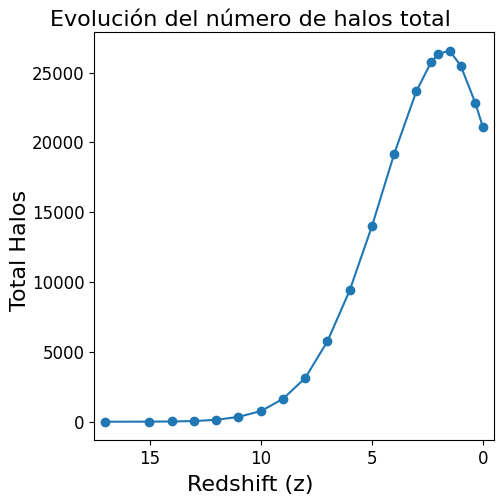
\includegraphics[scale = 0.5]{RunCanonica/TotalHalos_RunCanonica.png}
    \caption[Evolución del número de halos en un Universo $\Omega_\lambda = 0.691 $, $\Omega_0 = 0.309$]{\footnotesize Se muestra el numero de halos según el redshift y podemos observar como evoluciona el Universo en una cosmología $\Omega_\lambda = 0.691 $ y $\Omega_0 = 0.309$.}
    \label{fig:Canon_TotalHalos}
\end{figure}

La distribución de la masa para esta cosmología se observa en las figuras \ref{fig:Canon-MassDistSep} y \ref{fig:Canon-MassDist}. Los rangos de la masa se encuentran entre las $10^{10.11}M_\odot$ a $10^{14.32}M_\odot$ a lo largo de de la evolución del sistema. Las primeras estructuras, las que tienen $z$ altos, tenían masas menores a las $10^{11}M_\odot$ y las estructuras en $z$ pequeños la mayor parte de los halos tenían masas entre $10^{10.5}M_\odot$ y $10^{11.5}M_\odot$ con estructuras que alcanzan $10^{14.32}M_\odot$. Mientras, la figura \ref{fig:Canon-MassStats} nos muestra el comportamiento medio durante la evolución donde observamos que la masa media incrementa desde $10^{10.41}M_\odot$ con una desviación de $10^{0.11}M_\odot$ en $z=15$ hasta $10^{10.75}M_\odot$ con una desviación de $10^{0.49}M_\odot$ en $z=0$.

\begin{figure}[H]
    \centering
    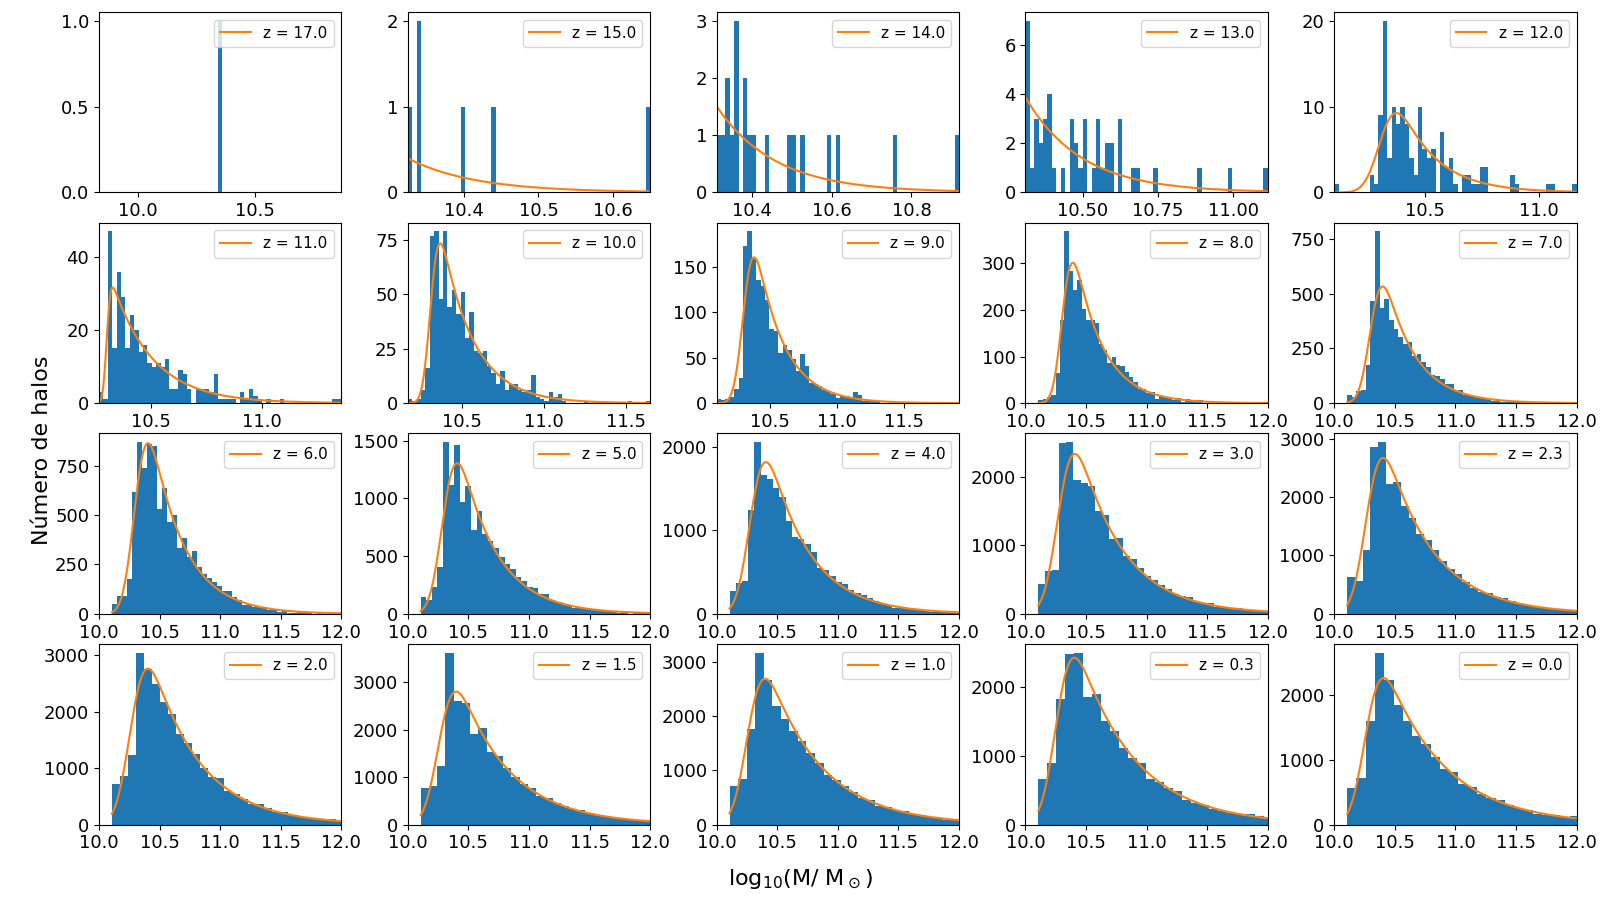
\includegraphics[width = 0.8\linewidth]{RunCanonica/Mass_Dist_RunCanonicaSep.png}
    \caption[Distribución de masa]{\footnotesize Tenemos la cantidad de halos en diferentes rangos de masa. Se muestran la distribución de la masa conforme evoluciona el Universo en una cosmología $\Omega_\lambda = 0.691 $ y $\Omega_0 = 0.309$. Se tienen las distribuciones en los diferentes redshifts empezando en $z=17$ en la parte superior izquierda y terminado en $z=0$ en la parte inferior derecha. Se observa como aumentan la cantidad de halos cada vez mas masivos.}
    \label{fig:Canon-MassDistSep}
\end{figure}

\begin{figure}[H]
    \centering
    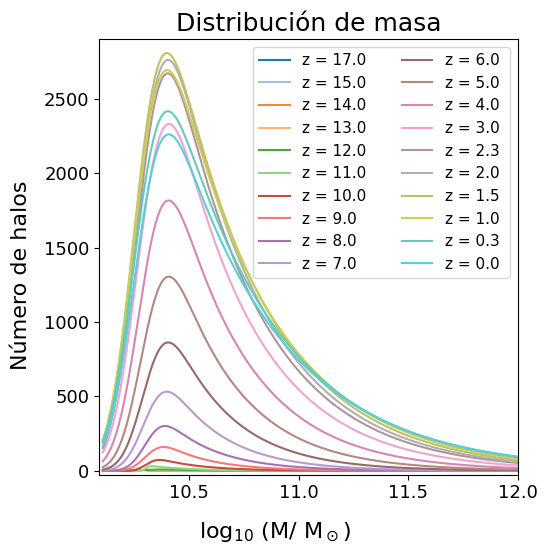
\includegraphics[width = 0.5\linewidth]{RunCanonica/Mass_Dist_RunCanonica.png}
    \caption[Comparación de distribución de masa]{\footnotesize Tenemos la cantidad de halos en los diferentes rangos de masa. Comparamos de las distribuciones de masa durante la evolución del Universo $\Omega_\lambda = 0.691 $, $\Omega_0 = 0.309$. Se muestra la cantidad de halos en un rango de masas. Se observa como crece la cantidad de halos de materia oscura, asi como el tamaño de estos.}
    \label{fig:Canon-MassDist}
\end{figure}

\begin{figure}[H]
    \centering
    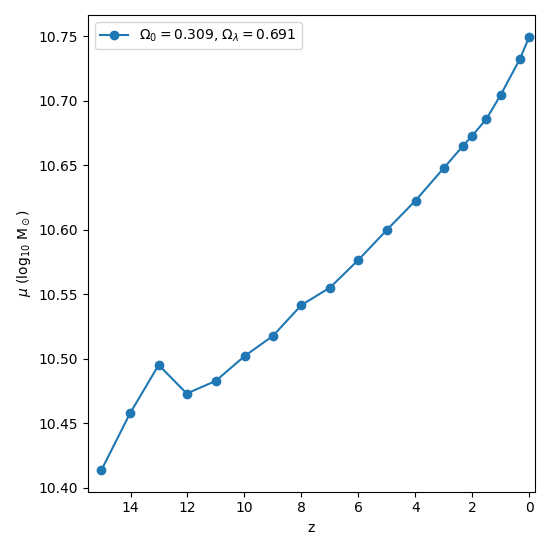
\includegraphics[width = 0.4\linewidth]{RunCanonica/MassMean_RunCanonica.png}
    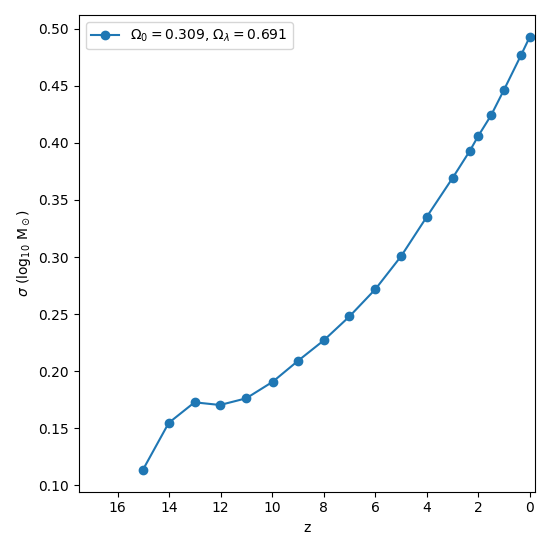
\includegraphics[width = 0.4\linewidth]{RunCanonica/MassStd_RunCanonica.png}
    \caption[Media y desviación estándar de la distribución de masa]{\footnotesize En la izquierda se muestra la masa media de los halos de materia oscura y se observa como cambia durante la evolución del Universo. En la derecha se muestra la desviación estándar de la masa, la cual nos muestra la variedad que hay de los halos de materia oscura, desde un z = 17 hasta un z = 0.}
    \label{fig:Canon-MassStats}
\end{figure}

En las figuras \ref{fig:Canon-HalfMassRadDistSep} y \ref{fig:Canon-HalfMassRadDist} podemos ver el radio que contiene la mitad de la masa de los halos a lo largo de la evolución del Universo. Vemos que los radios se encuentran entre los $10^{0.24}$kpc y $10^{2.69}$kpc donde los primeros halos tienen radios entre los $10^{0.24}$kpc y los $10^{1.01}$ y las estructuras mas recientes tienen la mayor parte de los halos en el rango de $10^{1.25}$kpc y los $10^{1.7}$kpc con halos que alcanzan hasta los $10^{2.69}kpc$. En la figura \ref{fig:Canon-HalfMassRadStats} vemos el crecimiento del radio medio desde $10^{0.44}$kpc con una desviación de $10^{0.06}$kpc en $z=15$ hasta un radio de $10^{1.47}$kpc con una desviación de $10^{0.19}$kpc en $z=0$.

\begin{figure}[H]
    \centering
    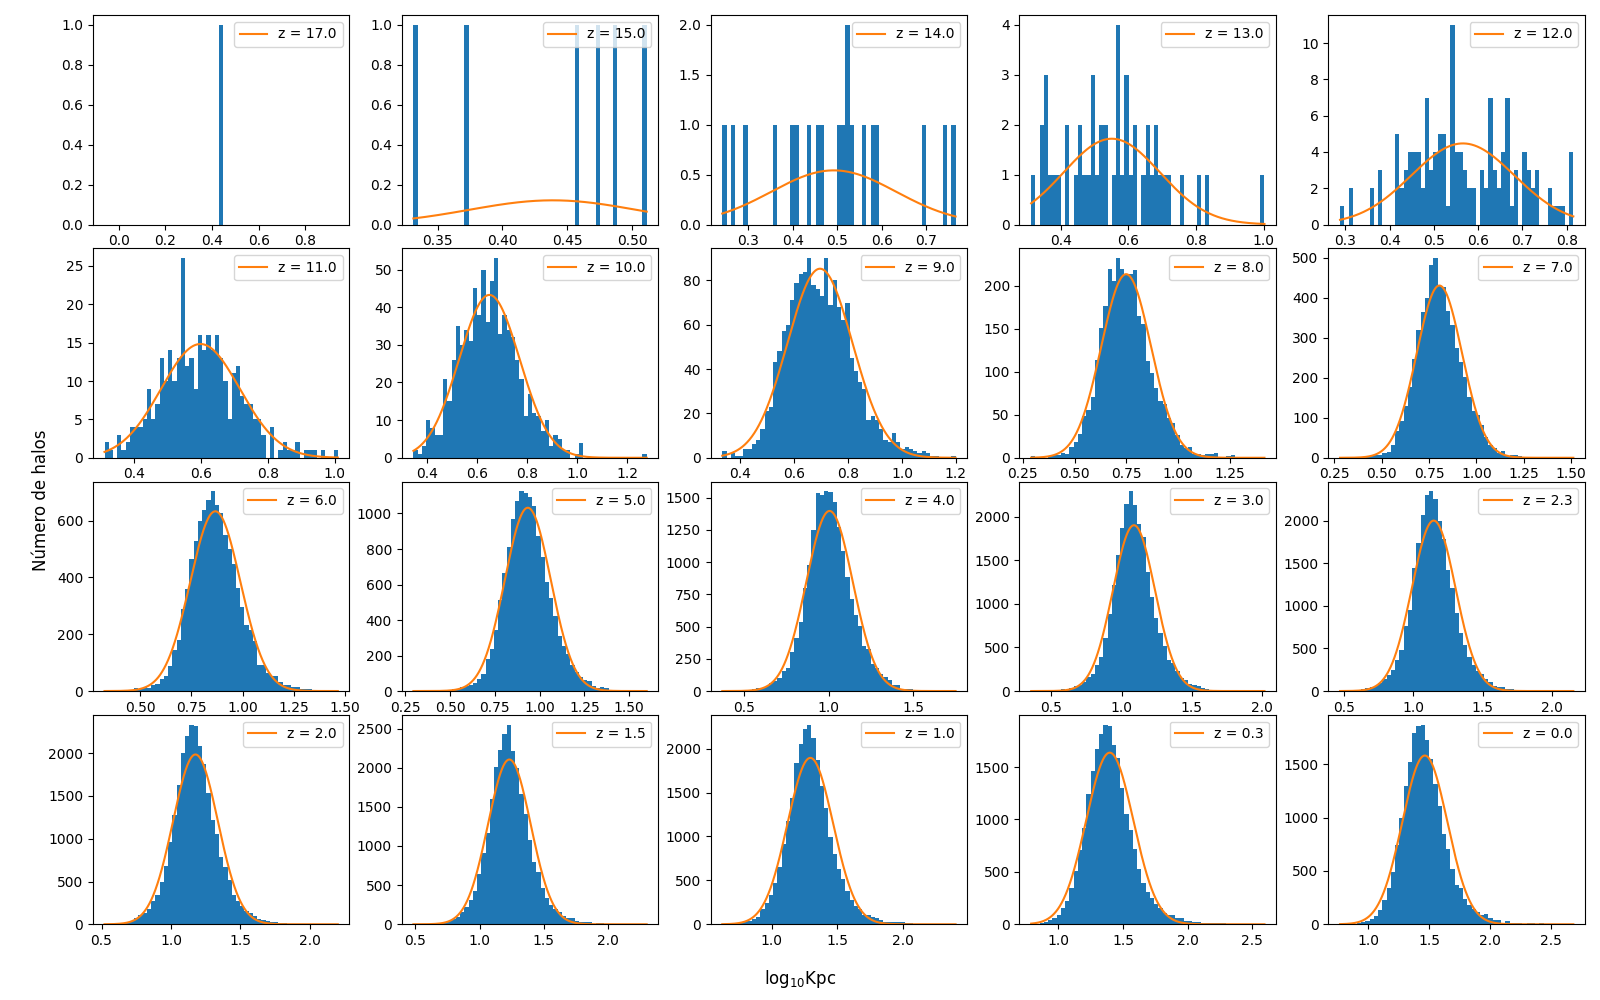
\includegraphics[width = 0.75\linewidth]{RunCanonica/HalfMassRad_Dist_RunCanonicaSep.png}
    \caption[Radio que contiene la mitad de la masa]{\footnotesize Se muestra la cantidad de halos que tiene el radio que contiene la mitad de la masa conforme evoluciona el Universo en una cosmología $\Omega_\lambda = 0.691 $ y $\Omega_0 = 0.309$. Se tienen las distribuciones en los diferentes redshifts empezando en $z=17$ en la parte superior izquierda y terminado en $z=0$ en la parte inferior derecha.}
    \label{fig:Canon-HalfMassRadDistSep}
\end{figure}

\begin{figure}[H]
    \centering
    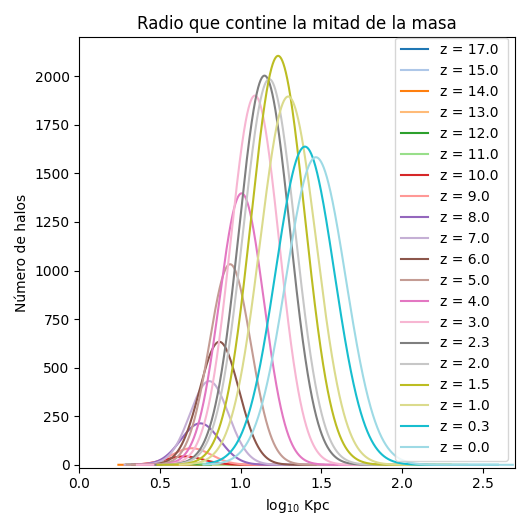
\includegraphics[width = 0.5\linewidth]{RunCanonica/HalfMassRad_Dist_RunCanonica.png}
    \caption[Distribución del radio que contiene la mitad de la masa]{\footnotesize Mostramos la cantidad de halos de materia oscura que tienen un radio que contiene la mitad de la masa en un Universo $\Omega_\lambda = 0.691 $, $\Omega_0 = 0.309$ desde un $z=17$ hasta un $z=0$.}
    \label{fig:Canon-HalfMassRadDist}
\end{figure}

\begin{figure}[H]
    \centering
    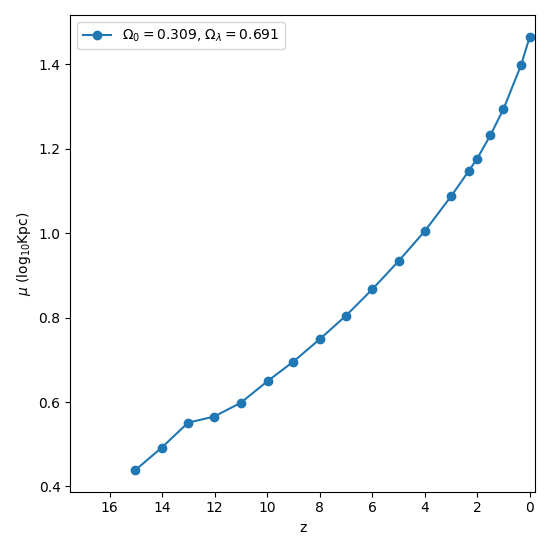
\includegraphics[width = 0.4\linewidth]{RunCanonica/HalfMassRad_Mean_RunCanonica.png}
    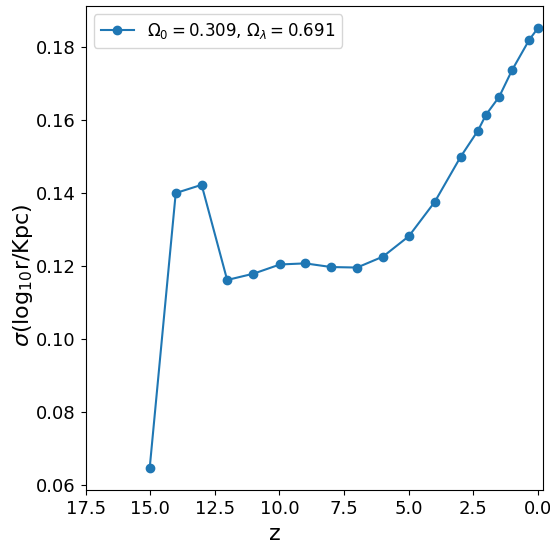
\includegraphics[width = 0.4\linewidth]{RunCanonica/HalfMassRad_Std_RunCanonica.png}
    \caption[Media y desviación estándar del radio de la mitad de la masa]{\footnotesize En la izquierda mostramos la media del radio que contiene la mitad de la masa de los halos de materia oscura y en la derecha se muestra su desviación estándar a lo largo de la evolución del Universo, desde un $z=17$ hasta un $z=0$.}
    \label{fig:Canon-HalfMassRadStats}
\end{figure}

Otra medida que utilizamos para dar una idea en el tamaño que tienen los halos es usando el radio donde tenemos la mayor velocidad radial. En las figuras \ref{fig:Canon-VMaxRadDistSep} y \ref{fig:Canon-VMaxRadDist} observamos que a lo largo de la evolución de las estructuras, tenemos halos con radios que van desde los $0.72$kpc hasta los $452.28$kpc. Vemos que la gran mayoría de los halos son halos con tamaños menores a $50$kpc con halos que alcanzan hasta los $452.28$kpc mas al presente y menores a $10$kpc con estructuras que alcanzan $9.83$kpc en los redshifts mas altos. En la figura \ref{fig:Canon-VMaxRadStats} vemos que la media va desde los $2.45$kpc con una desviación de $0.88$kpc en $z=15$ hasta $27.60$kpc con una desviación de $15.69$kpc en $z=0$.

\begin{figure}[H]
    \centering
    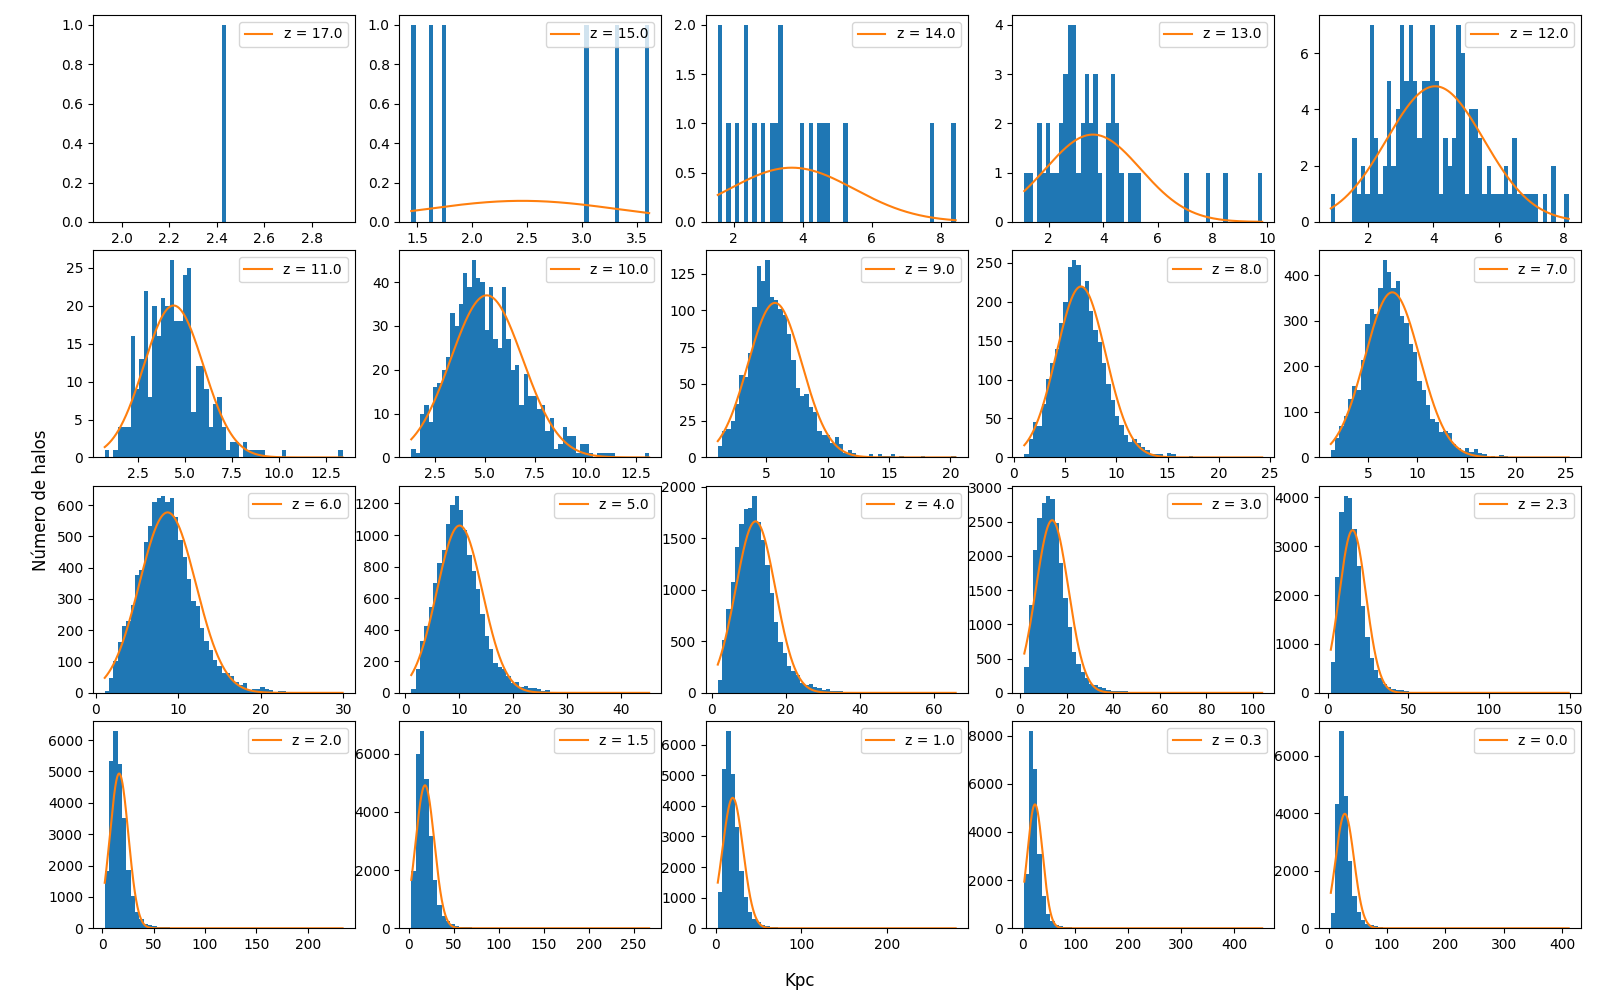
\includegraphics[width = 0.75\linewidth]{RunCanonica/VMaxRad_Dist_RunCanonicaSep.png}
    \caption[Radio donde se alcanza la velocidad máxima radial]{\footnotesize Se muestra el radio donde se alcanza la velocidad máxima radial conforme evoluciona el Universo en una cosmología $\Omega_\lambda = 0.691 $ y $\Omega_0 = 0.309$. Se tienen las distribuciones en los diferentes redshifts empezando en $z=17$ en la parte superior izquierda y terminado en $z=0$ en la parte inferior derecha.}
    \label{fig:Canon-VMaxRadDistSep}
\end{figure}

\begin{figure}[H]
    \centering
    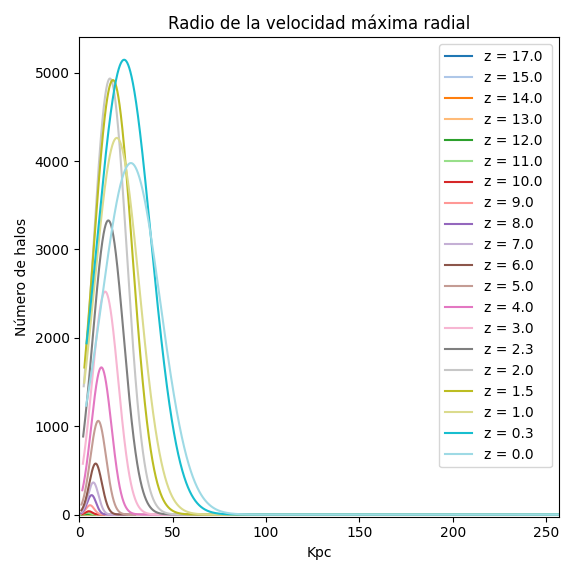
\includegraphics[width = 0.5\linewidth]{RunCanonica/VMaxRad_Dist_RunCanonica.png}
    \caption[Distribución del radio donde se alcanza la velocidad máxima radial]{\footnotesize Se muestra la cantidad de halos de materia oscura con el radio donde se alcanza la velocidad máxima radial en un Universo $\Omega_\lambda = 0.691 $, $\Omega_0 = 0.309$.}
    \label{fig:Canon-VMaxRadDist}
\end{figure}

\begin{figure}[H]
    \centering
    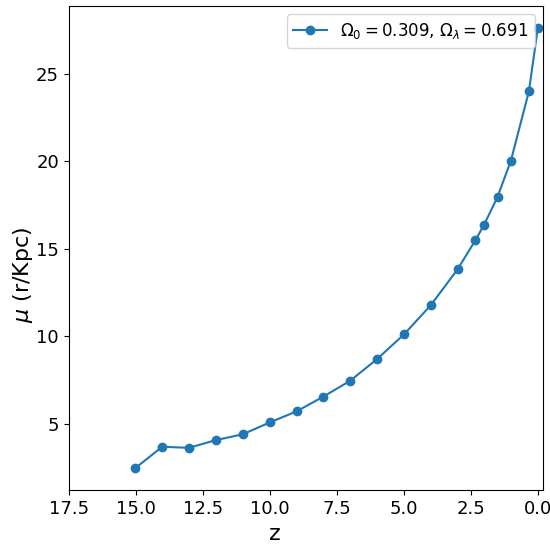
\includegraphics[width = 0.4\linewidth]{RunCanonica/VMaxRad_Mean_RunCanonica.png}
    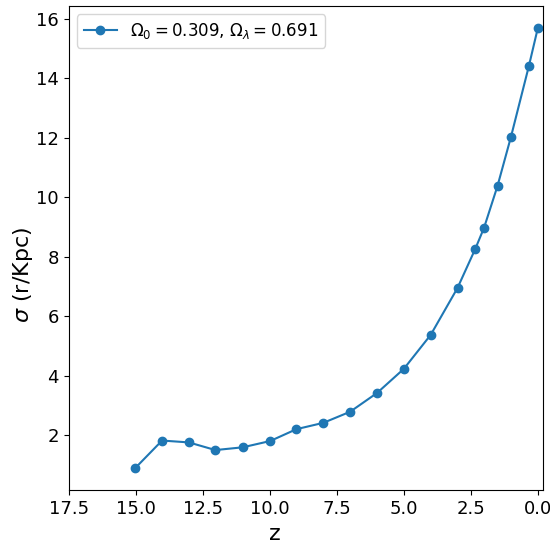
\includegraphics[width = 0.4\linewidth]{RunCanonica/VMaxRad_Std_RunCanonica.png}
    \caption[Media y desviación estándar del Radio donde se alcanza la velocidad máxima radial]{\footnotesize En la izquierda mostramos la media del radio donde se alcanza la velocidad máxima radial de los halos de materia oscura y en la derecha se muestra su desviación estándar a lo largo de la evolución del Universo, desde un $z=17$ hasta un $z=0$.}
    \label{fig:Canon-VMaxRadStats}
\end{figure}

Pasando a las velocidades, empezando con la velocidad circular máxima. Podemos apreciar que las velocidades circulares van de los rangos de los $22.82$km/s hasta los $1001.91$km/s donde vemos la gran mayoría de los halos en los rangos de $100$km/s y $175$km/s para los $z$ altos y entre los $50$km/s y $175$km/s mas al presente, como se muestra en las figuras \ref{fig:Canon-VelMaxDistSep} y \ref{fig:Canon-VelMaxDist}. Lo que podemos ver en la figura \ref{fig:Canon-VelMaxStats} es que la velocidad  media disminuye rápidamente desde $150.13$km/s con una desviación de $26.76$km/s en $z=15$ hasta que alcanza $74.77$km/s con una desviación de $33.90$km/s en $z=0$.

% Pasando a las velocidades, empezando con la velocidad circular máxima, en las figuras \ref{fig:VelMaxDistSep} y \ref{fig:VelMaxDist} podemos ver que un pequeña parte de los halos tienen velocidades mayores a $200$ km/s a lo largo de la evolución del Universo. La mayor parte tienen velocidades entre $40$ y $150$km/s. Algo que se observa en la figura \ref{fig:VelMaxStats} es que la velocidad media disminuye conforme avanza el tiempo, pero también vemos un aumento en la diversidad de velocidades que hay. La media en un universo temprano se encontraba entre los $130$ y $150$ km/s con variaciones entre $10$ y $30$ km/s. En el presente tenemos una media de $74.7$ km/s con desviación de $33.9$ km/s. 

\begin{figure}[H]
    \centering
    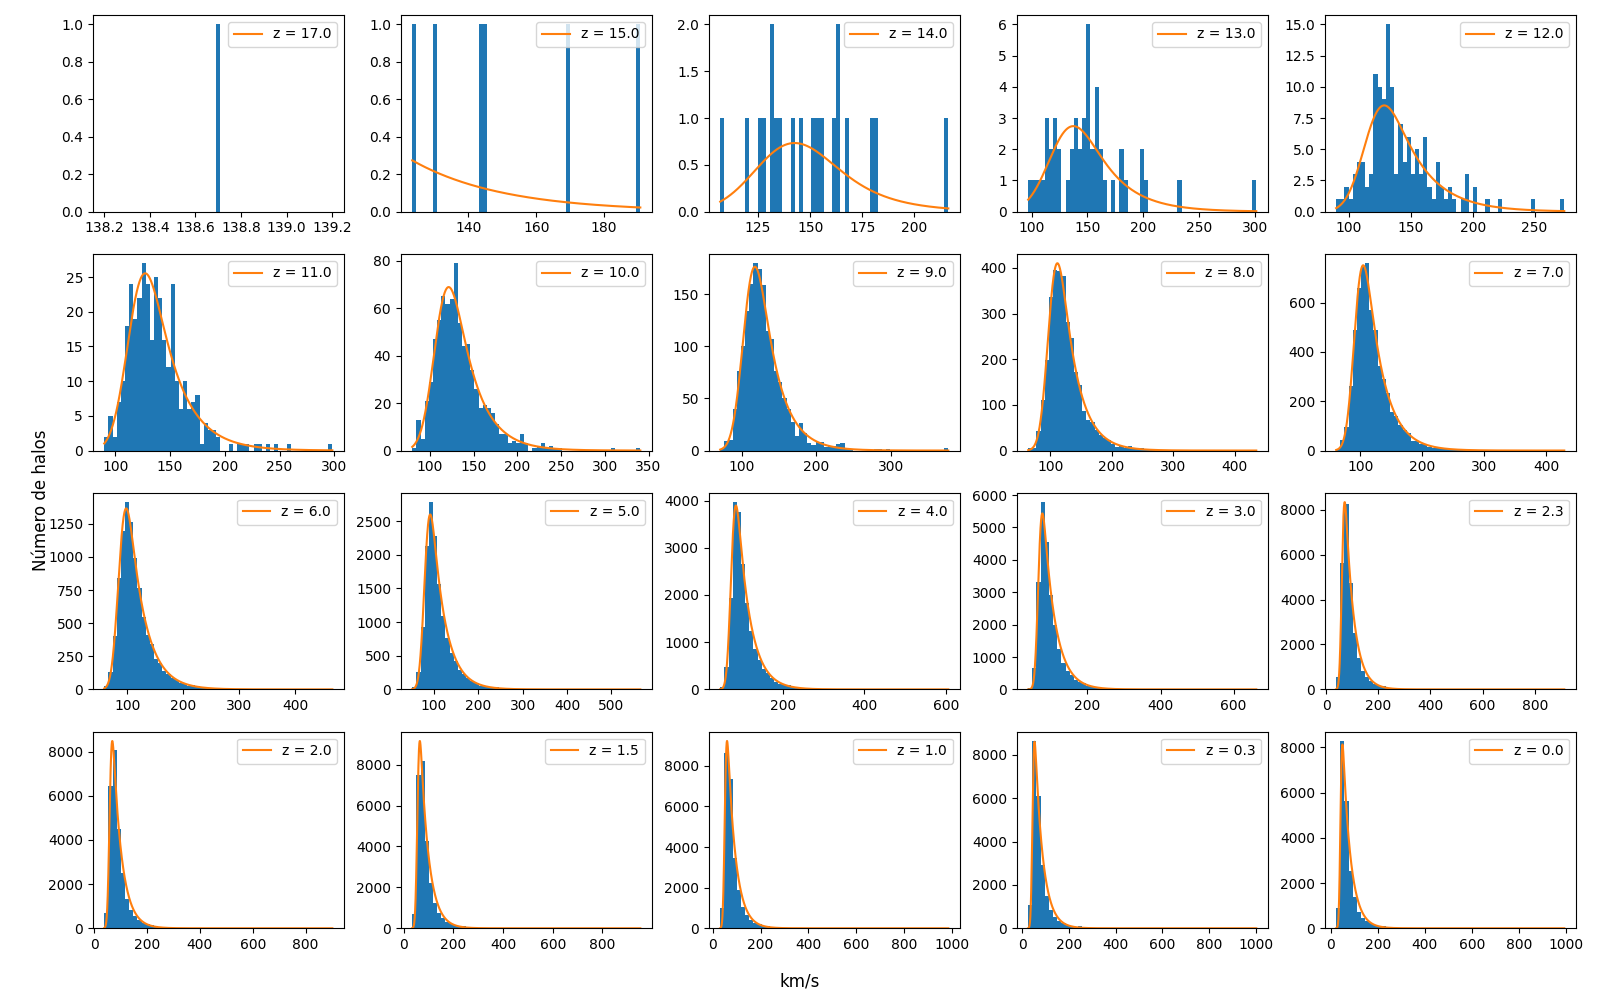
\includegraphics[width = 0.75\linewidth]{RunCanonica/VelMax_Dist_RunCanonicaSep.png}
    \caption[Velocidad circular máxima]{\footnotesize Se muestra la velocidad circular máxima conforme evoluciona el Universo en una cosmología $\Omega_\lambda = 0.691 $ y $\Omega_0 = 0.309$. Se tienen las distribuciones en los diferentes redshifts empezando en $z=17$ en la parte superior izquierda y terminado en $z=0$ en la parte inferior derecha.}
    \label{fig:Canon-VelMaxDistSep}
\end{figure}

\begin{figure}[H]
    \centering
    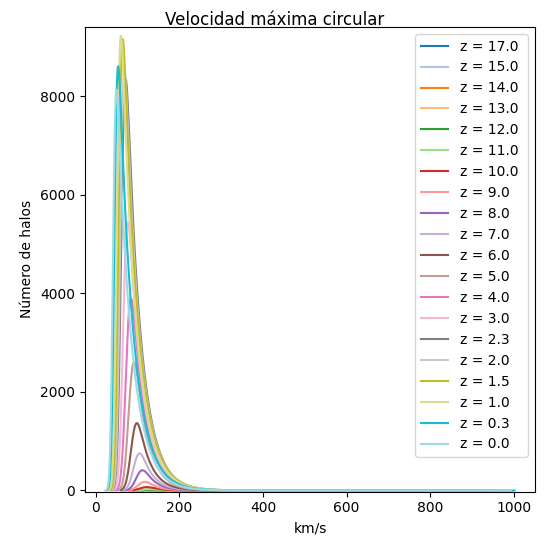
\includegraphics[width = 0.5\linewidth]{RunCanonica/VelMax_Dist_RunCanonica.png}
    \caption[Distribución de la velocidad circular máxima]{\footnotesize Mostramos la cantidad de halos de materia oscura en los diferentes rangos de velocidad circular máxima en un Universo $\Omega_\lambda = 0.691 $, $\Omega_0 = 0.309$.}
    \label{fig:Canon-VelMaxDist}
\end{figure}

\begin{figure}[H]
    \centering
    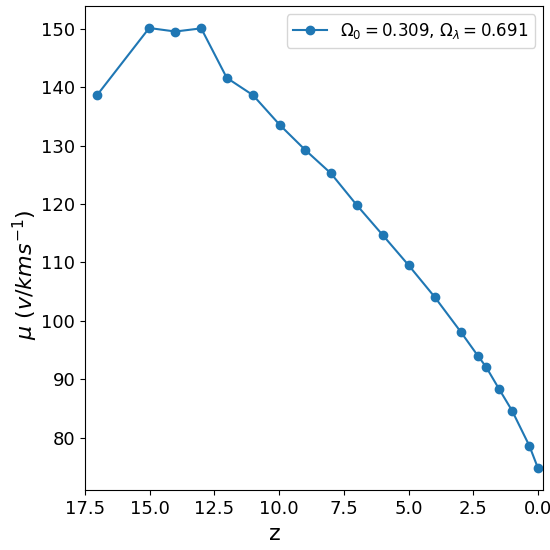
\includegraphics[width = 0.4\linewidth]{RunCanonica/VelMax_Mean_RunCanonica.png}
    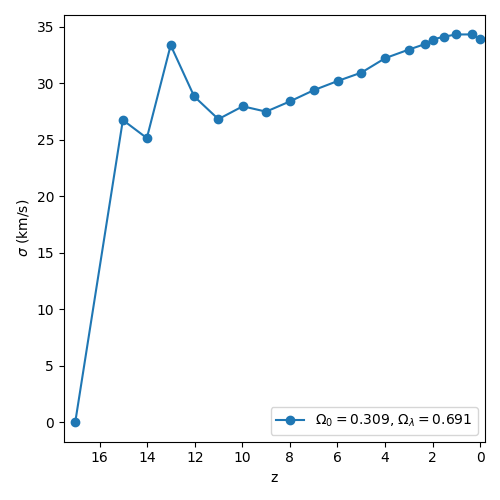
\includegraphics[width = 0.4\linewidth]{RunCanonica/VelMax_Std_RunCanonica.png}
    \caption[Media y desviación estándar de la velocidad circular máxima]{\footnotesize En la izquierda mostramos la media de la velocidad circular máxima de los halos de materia oscura y en la derecha se muestra su desviación estándar a lo largo de la evolución del Universo.}
    \label{fig:Canon-VelMaxStats}
\end{figure}

Ahora hablemos de la dispersion de las velocidades de los halos de materia oscura. La dispersión de velocidades de estos halos esta en los rangos de $12.78$km/s a los $619.79$km/s a lo largo de la evolución de los halos. Vemos en las figuras \ref{fig:Canon-VelDispDistSep} y \ref{fig:Canon-VelDispDist} que en los $z$ altos vemos que que la mayor parte de los halos se encuentran en el rango de los $60$km/s a los $100$km/s con picos en los $183.94$km/s, mientras que en los $z$ bajos vemos los rango que van de $50$km/s y $80$km/s con los picos entre los $355.62$km/s y $619.79$km/s. En la figura \ref{fig:Canon-VelDispStats} observamos que la dispersión de velocidades media disminuye desde los $85.25$km/s con una desviación de $13.09$km/s en $z=15$ a $37.08$km/s con una desviación de $18.69$km/s en $z=0$.

% Para terminar de hablar de la dinámica interna del halo, las figuras \ref{fig:VelDispDistSep} \ref{fig:VelDispDist} nos muestran las distribuciones de la dispersión de velocidades. Observamos un comportamiento similar a la velocidad máxima circular, donde vemos casos pocos situaciones con dispersiones mayores de $150$ km/s. Ademas, si observamos la figura \ref{fig:VelDispStats}, podemos apreciar una disminución en la dispersion de velocidades media similar a la media de la velocidad circular máxima. En este caso vemos que la dispersión de velocidades media varia desde $86.5$ km/s en el pasado, hasta $37$ km/s en el presente. 

\begin{figure}[H]
    \centering
    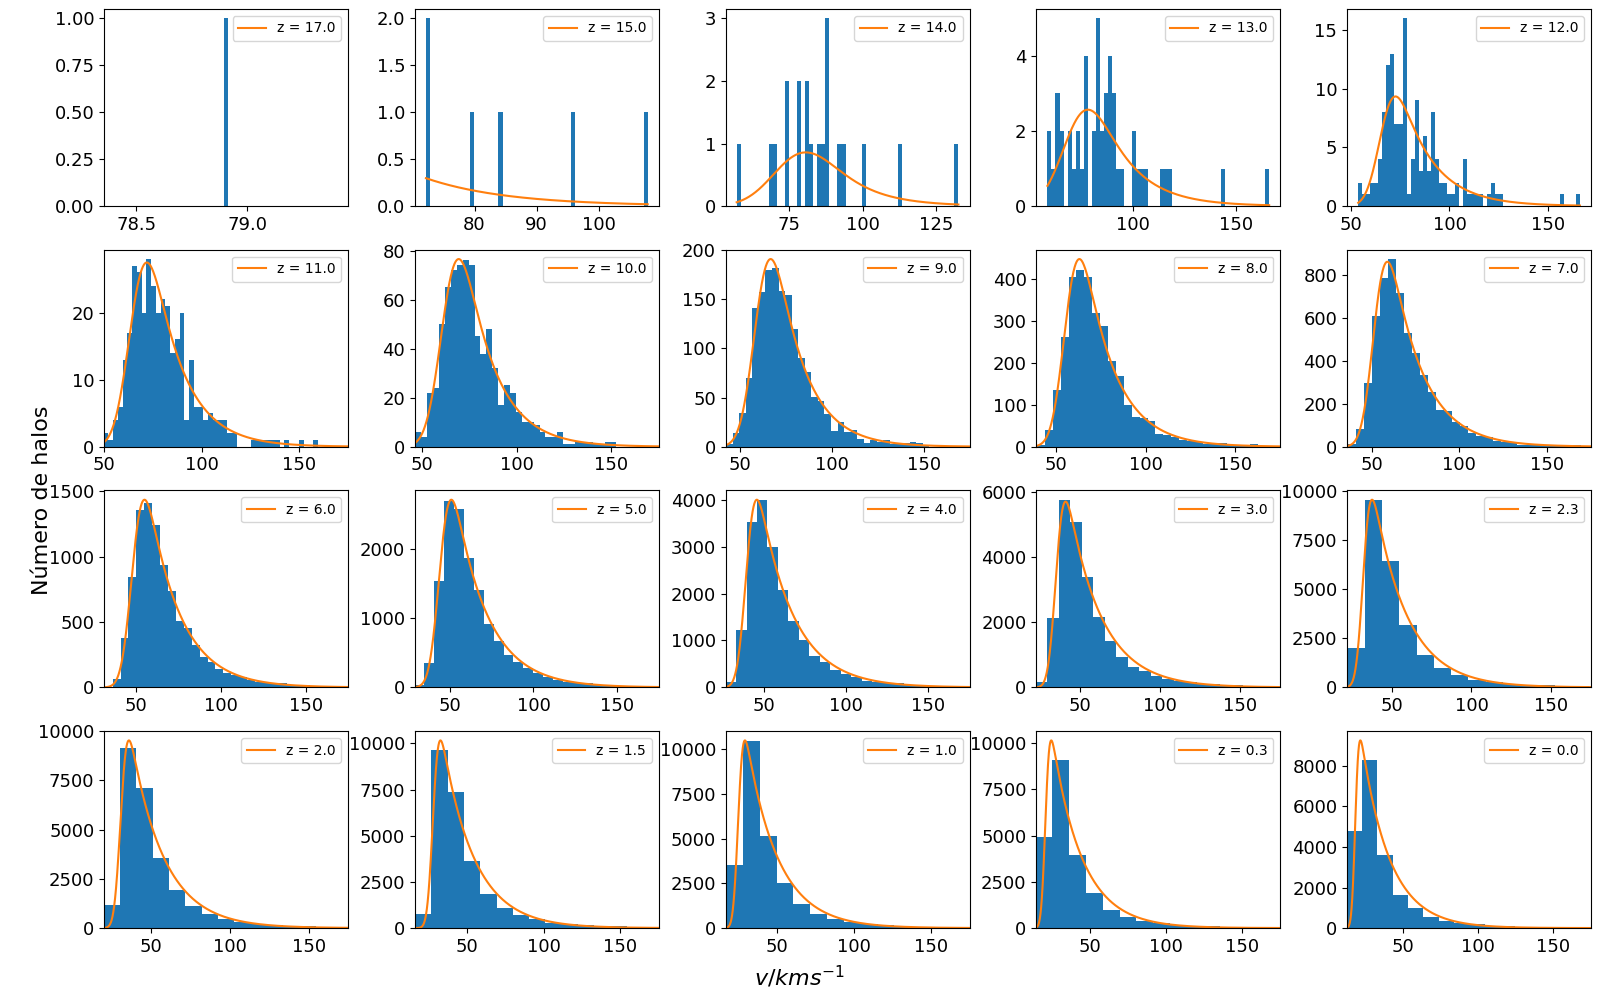
\includegraphics[width = 0.75\linewidth]{RunCanonica/VelDisp_Dist_RunCanonicaSep.png}
    \caption[Dispersión de velocidades]{\footnotesize Se muestra la dispersión de velocidades conforme evoluciona el Universo en una cosmología $\Omega_\lambda = 0.691 $ y $\Omega_0 = 0.309$.Se tienen las distribuciones en los diferentes redshifts empezando en $z=17$ en la parte superior izquierda y terminado en $z=0$ en la parte inferior derecha.}
    \label{fig:Canon-VelDispDistSep}
\end{figure}

\begin{figure}[H]
    \centering
    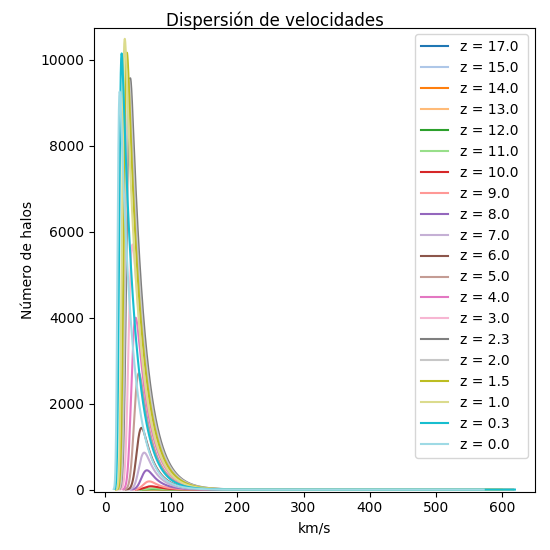
\includegraphics[width = 0.5\linewidth]{RunCanonica/VelDisp_Dist_RunCanonica.png}
    \caption[Distribución de la dispersión de velocidades]{\footnotesize Mostramos la dispersion de velocidades de los halos de materia oscura en un Universo $\Omega_\lambda = 0.691 $, $\Omega_0 = 0.309$.}
    \label{fig:Canon-VelDispDist}
\end{figure}

\begin{figure}[H]
    \centering
    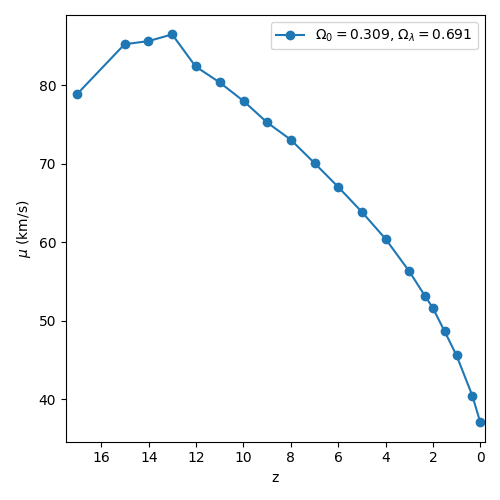
\includegraphics[width = 0.4\linewidth]{RunCanonica/VelDisp_Mean_RunCanonica.png}
    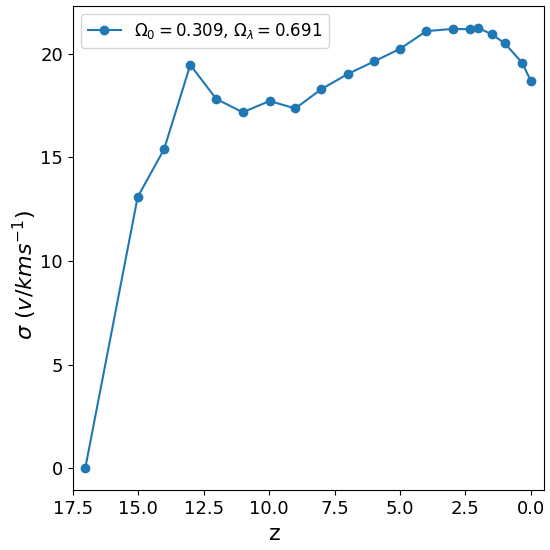
\includegraphics[width = 0.4\linewidth]{RunCanonica/VelDisp_Std_RunCanonica.png}
    \caption[Media y desviación estándar de la dispersión de velocidades]{\footnotesize En la izquierda mostramos la media de la dispersión de velocidades de los halos de materia oscura y en la derecha se muestra su desviación estándar a lo largo de la evolución del Universo.}
    \label{fig:Canon-VelDispStats}
\end{figure}

Finalmente, la figura \ref{fig:CanonRunDensityMap} muestra a lo que conocemos como la \emph{Cosmic Web} vista desde un plano. Se ve el mapa de densidad de la simulación del Universo en diferentes redshifts. En los redshift altos (viendo mas al pasado) se observan nubes difusas donde no hay una estructura, mientras que los redshift bajos (mas al presente) se observan estructuras mejor definidos y con el tiempo vemos que hay un aumento en la cantidad de estructura que se observa.

\begin{figure}[H]
    \centering

    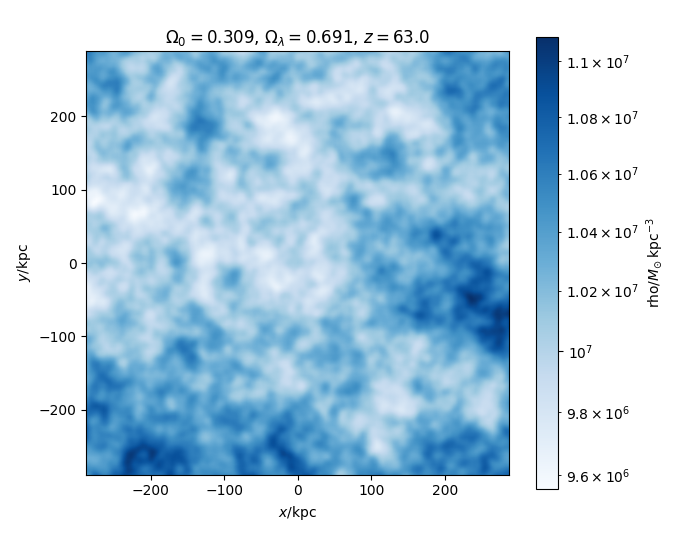
\includegraphics[width = 0.33\linewidth]{RunCanonica/RunCanonZ63Rho.png}   %snap 000 z=63
    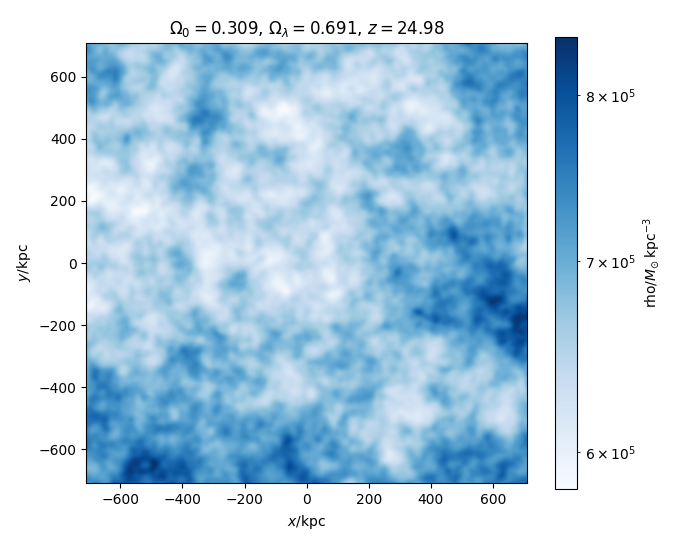
\includegraphics[width = 0.33\linewidth]{RunCanonica/RunCanonZ25Rho.png}   %snap 005 z=25
    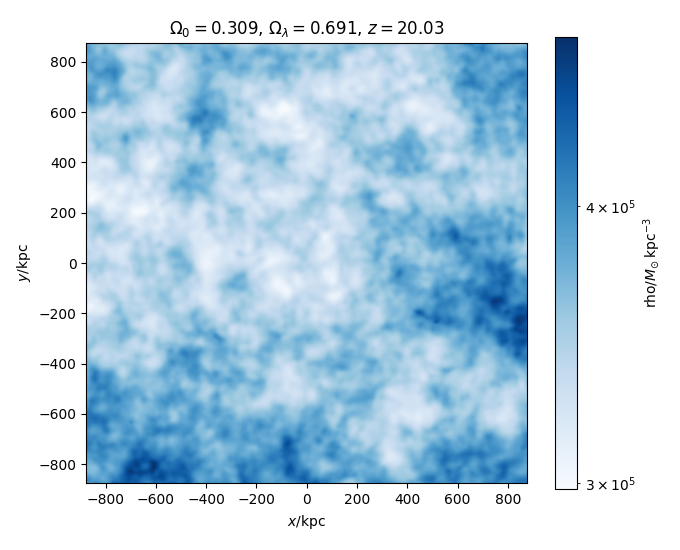
\includegraphics[width = 0.32\linewidth]{RunCanonica/RunCanonZ20Rho.png}   %snap 010 z=20
    \\
    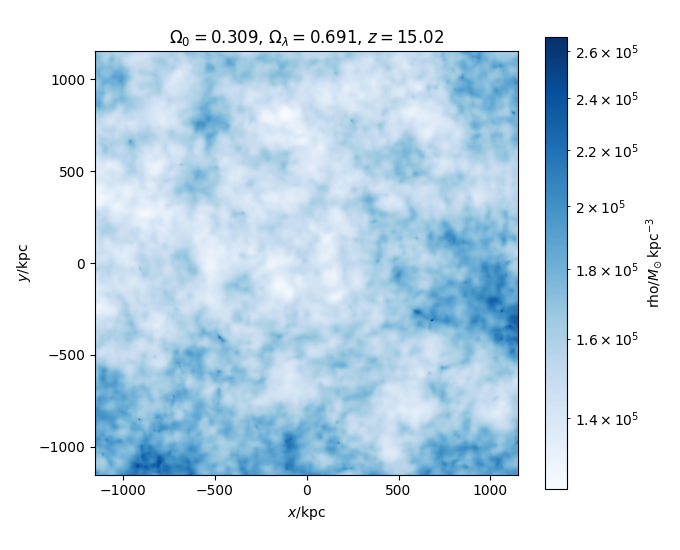
\includegraphics[width = 0.33\linewidth]{RunCanonica/RunCanonZ15Rho.png}   %snap 015 z=15
    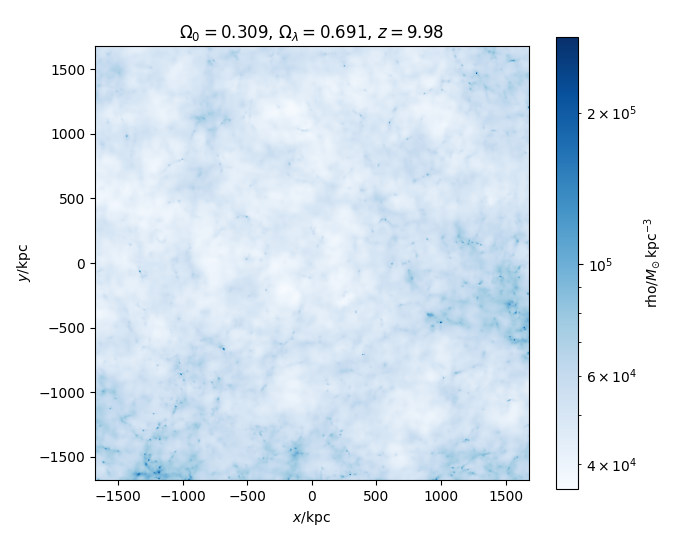
\includegraphics[width = 0.33\linewidth]{RunCanonica/RunCanonZ10Rho.png}   %snap 020 z=10
    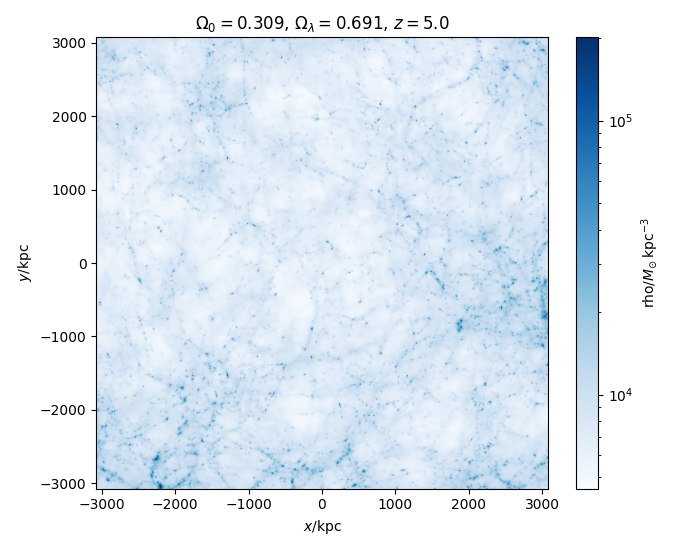
\includegraphics[width = 0.32\linewidth]{RunCanonica/RunCanonZ5Rho.png}    %snap 025 z=5
    \\
    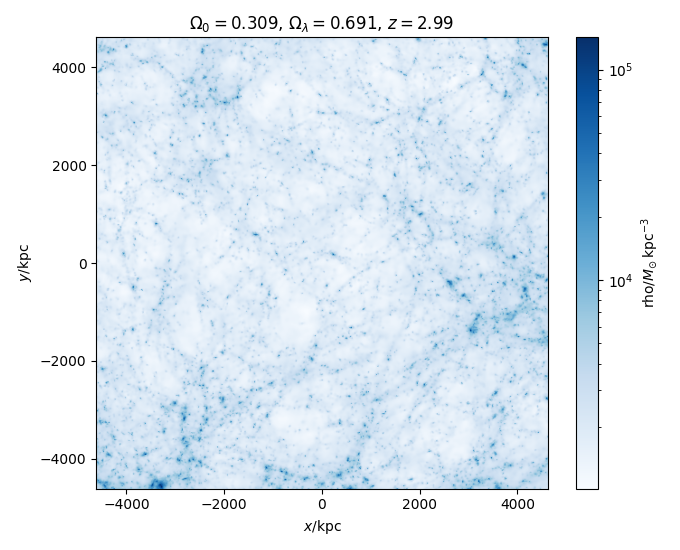
\includegraphics[width = 0.33\linewidth]{RunCanonica/RunCanonZ3Rho.png}    %snap 027 z=3
    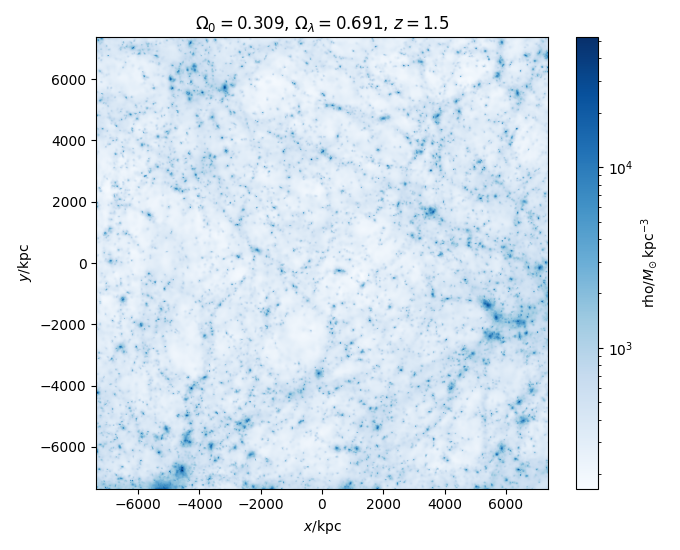
\includegraphics[width = 0.33\linewidth]{RunCanonica/RunCanonZ1_5Rho.png}  %snap 030 z=1.5
    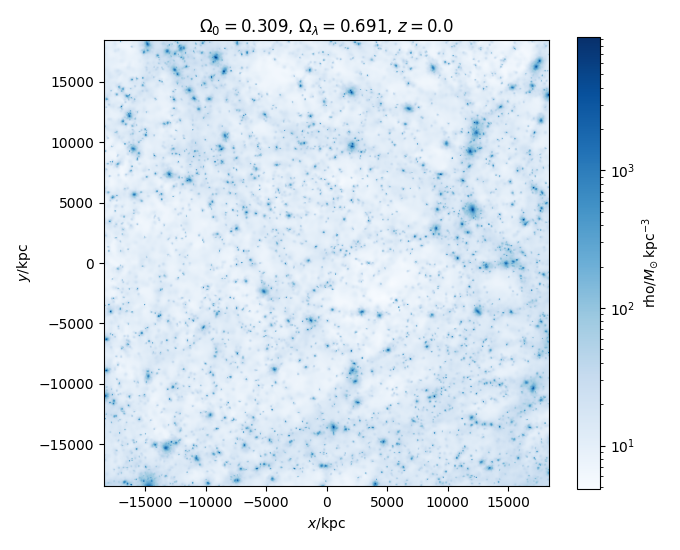
\includegraphics[width = 0.32\linewidth]{RunCanonica/RunCanonZ0Rho.png}    %snap 033 z=0
    \caption[Mapa de densidad de un Universo en en diferentes redshift]{ \footnotesize Mapa de densidad de la simulación en diferentes redshifts de una cosmología $\Omega_\lambda = 0.691 $, $\Omega_0 = 0.309$. }
    \label{fig:CanonRunDensityMap}
\end{figure}

%====================================================================================================================
%=====================================  RUN INVERTIDA  ==============================================================
%====================================================================================================================
\subsection{Universo con cosmología  \texorpdfstring{$\Omega_\lambda = 0.309$, $\Omega_0 = 0.691$ }{Omega lambda = 0.309, Omega 0 = 0.691} }
Hemos estudiado un Universo con las densidades mas aceptadas, pero como cambia si las densidades cambian, para este caso que sucede si invertimos las densidades pero dejamos el Universo plano. Primeramente podemos apreciar en la figura \ref{fig:Invertida-TotalHalos} que los halos se empiezan a formar en redshift $z=14$ pero tiene un comportamiento similar a la cosmología anterior, teniendo el pico en la cantidad de halos alrededor del redshift $z=2$. 

\begin{figure}[H]
    \centering
    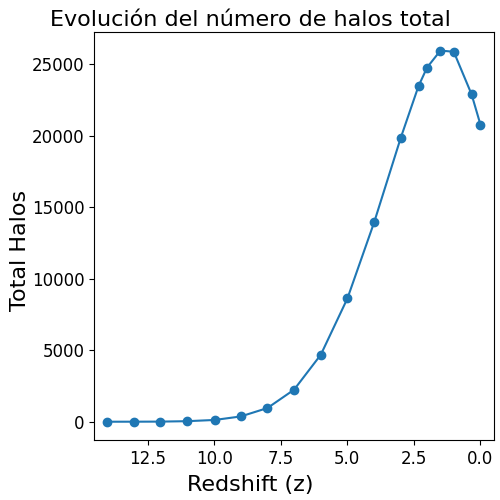
\includegraphics[scale = 0.5]{RunInvertida/TotalHalos_RunInvertida.png}
    \caption[Evolución del número de halos en un Universo $\Omega_\lambda = 0.309 $, $\Omega_0 = 0.691$]{\footnotesize Se muestra el numero de halos y como cambia la cantidad conforme evoluciona el Universo en una cosmología $\Omega_\lambda = 0.309 $ y $\Omega_0 = 0.691$.}    
    \label{fig:Invertida-TotalHalos}
\end{figure}

La distribución de masa de los halos se ve en la figura \ref{fig:Invertida-MassDist} a largo de la evolución. Podemos ver poca estructura con masas mayores a $10^{12}M_\odot$ y mayor parte de la masa entre $10^{10.3}$ y $10^{11}M_\odot$. Ademas en  \ref{fig:Invertida-MassStats} vemos que la media muestra un incremento en la masa de los halos, el que va de $10^{10.8} M\odot$ en $z=13$ hasta $10^{11.1}M_\odot$ en $z=0$. Esto es un incremento de aproximadamente un orden de magnitud. Mientras la desviación tiene un incremento aproximado de $10^{0.1}M_\odot$ en $z=13$ a $10^{0.5}M_\odot$ en $z=0$. 

\begin{figure}[H]
    \centering
    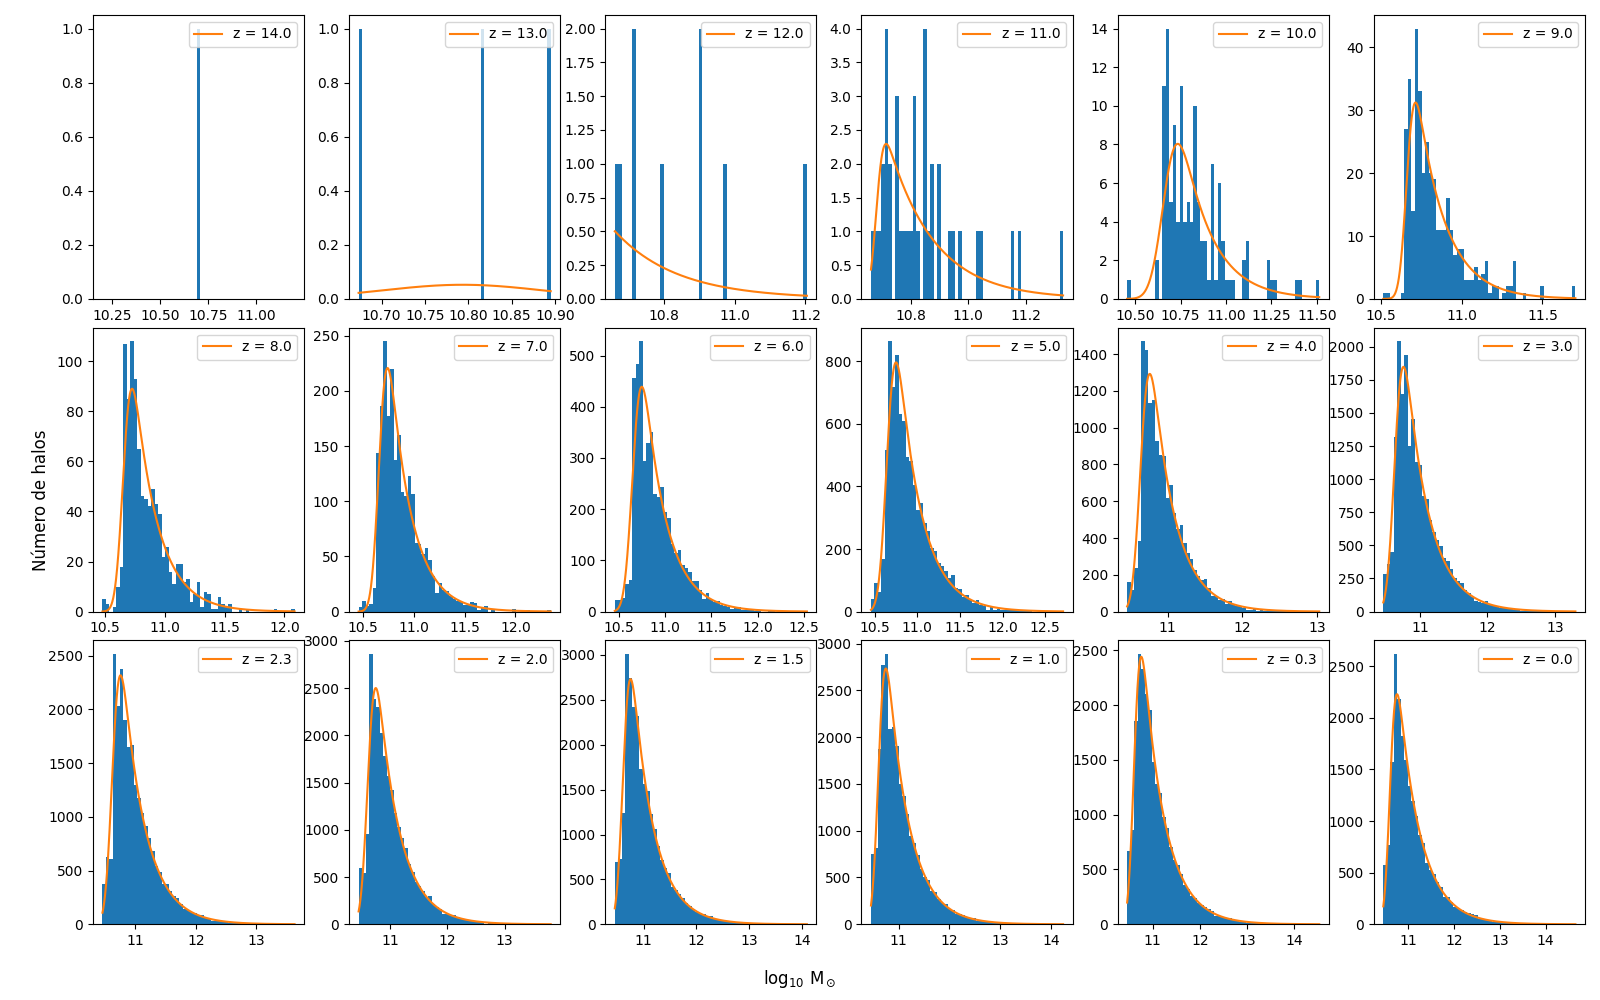
\includegraphics[width = 0.8\linewidth]{RunInvertida/Mass_Dist_RunInvertidaSep.png}
    \caption[Distribución de masa]{\footnotesize Se muestra la distribución de la masa conforme evoluciona el Universo en una cosmología $\Omega_\lambda = 0.309 $ y $\Omega_0 = 0.691$. Se observa como aumentan la cantidad de halos cada vez mas masivos.}
    \label{fig:Invertida-MassDistSep}
\end{figure}

\begin{figure}[H]
    \centering
    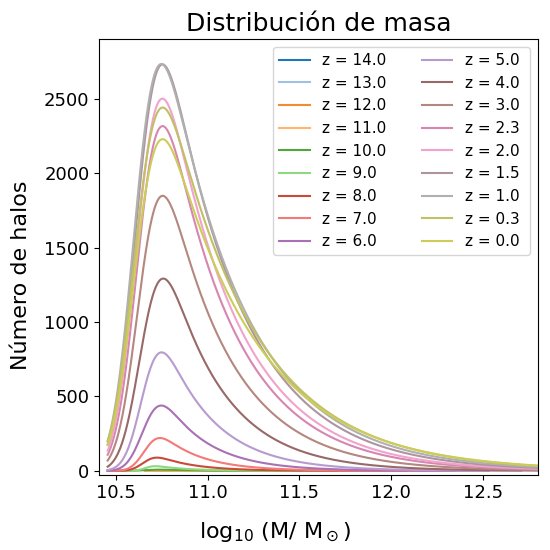
\includegraphics[width = 0.5\linewidth]{RunInvertida/Mass_Dist_RunInvertida.png}
    \caption[Comparación de distribución de masa]{\footnotesize Comparación de las distribuciones de masa durante la evolución del Universo $\Omega_\lambda = 0.309 $, $\Omega_0 = 0.691$. Se observa como crece la cantidad de halos de materia oscura, asi como el tamaño de estos.}
    \label{fig:Invertida-MassDist}
\end{figure}

\begin{figure}[H]
    \centering
    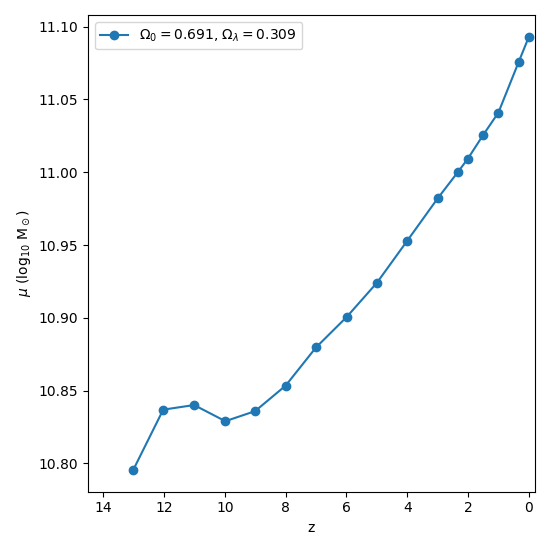
\includegraphics[width = 0.4\linewidth]{RunInvertida/MassMean_RunInvertida.png}
    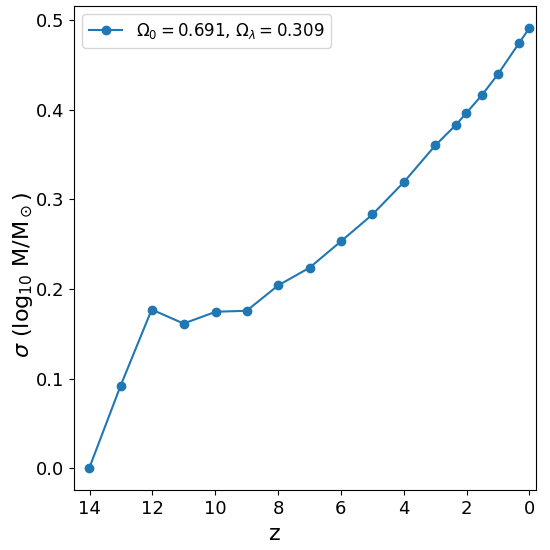
\includegraphics[width = 0.4\linewidth]{RunInvertida/MassStd_RunInvertida.png}
    \caption[Media y desviación estándar de la distribución de masa]{\footnotesize En la izquierda se muestra la masa media de los halos de materia oscura y se observa como cambia durante la evolución del Universo. En la derecha se muestra la desviación estándar de la masa, la cual nos muestra la variedad que hay de los halos de materia oscura.}
    \label{fig:Invertida-MassStats}
\end{figure}

Ahora hablemos del tamaño de estas estructuras, empezando con el radio que contiene la mitad de la masa. En la figura \ref{fig:Invertida-HalfMassRadDistSep} y \ref{fig:Invertida-HalfMassRadDist} vemos que tenemos halos que tienen radios desde $10^{0.35}$ kpc hasta $10^{2.5}$ kpc a lo largo de la evolución de los halos. Vemos en la figura \ref{fig:Invertida-HalfMassRadStats} que el radio crece con el tiempo teniendo un crecimiento desde $10^{0.53}$kpc en las primeras estructuras hasta $10^{1.5}$kpc en el presente. También vemos que las primeras estructuras tienen desviaciones de entre $10^{0.08}$ y $10^{0.15}$kpc mientras que las mas recientes estaban entre $10^{0.15}$ y $10^{0.19}$ kpc.

\begin{figure}[H]
    \centering
    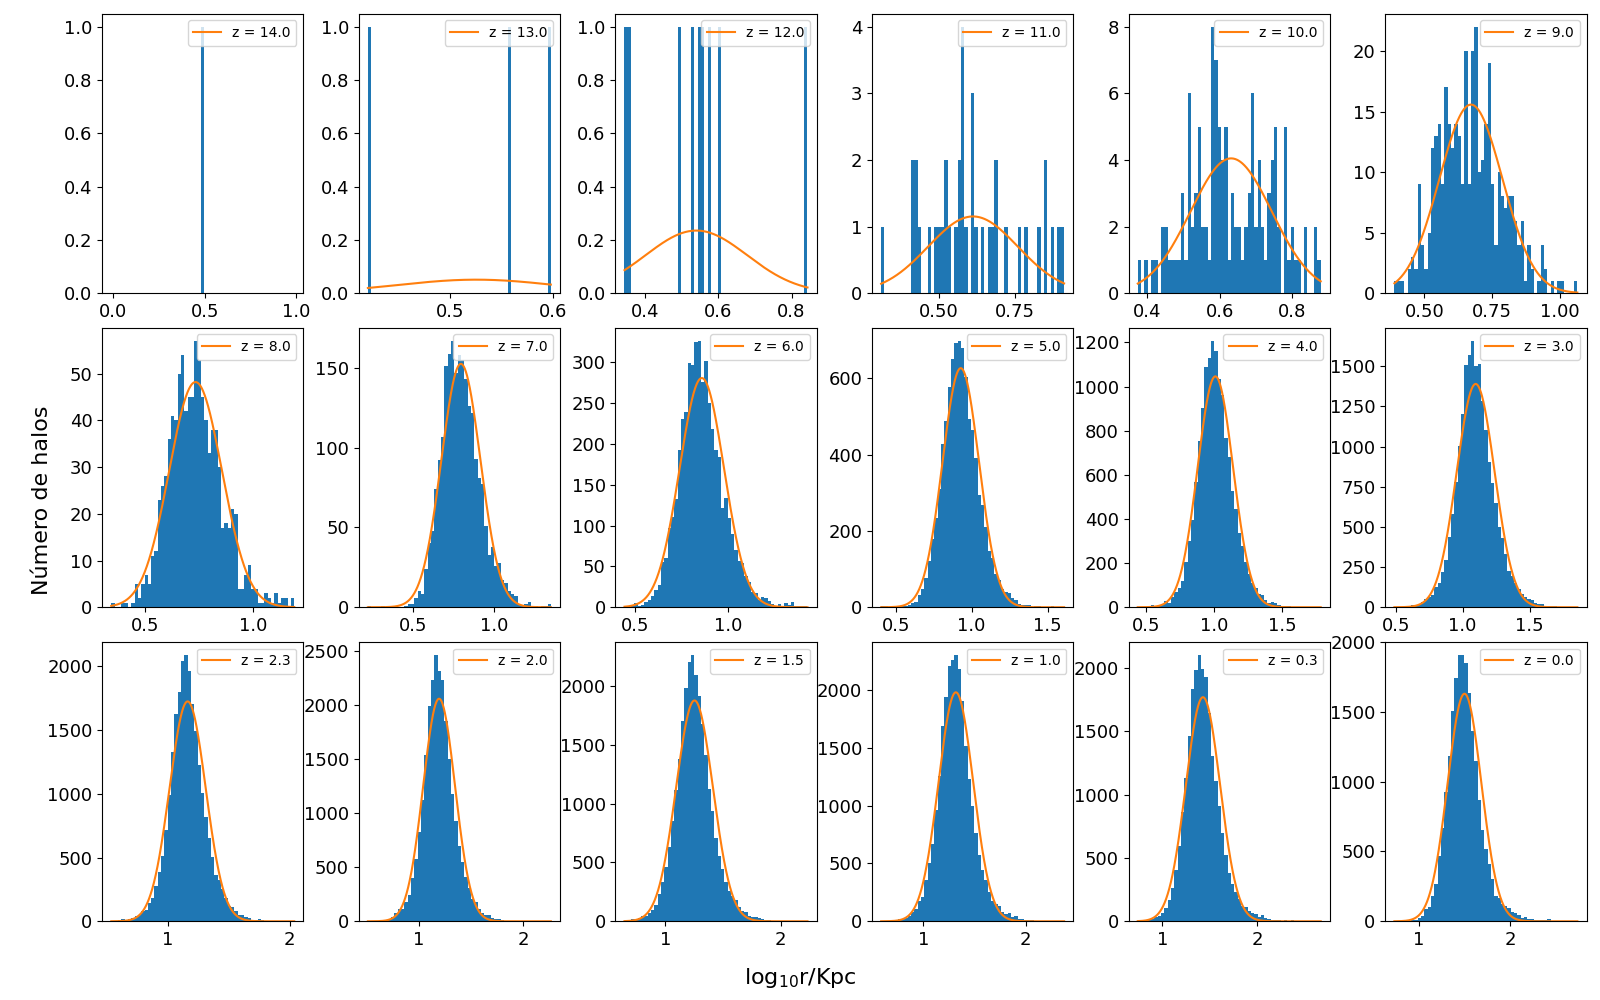
\includegraphics[width = 0.75\linewidth]{RunInvertida/HalfMassRad_Dist_RunInvertidaSep.png}
    \caption[Radio que contiene la mitad de la masa]{\footnotesize Se muestra el radio que contiene la mitad de la masa conforme evoluciona el Universo en una cosmología $\Omega_\lambda = 0.309 $ y $\Omega_0 = 0.691$.}
    \label{fig:Invertida-HalfMassRadDistSep}
\end{figure}

\begin{figure}[H]
    \centering
    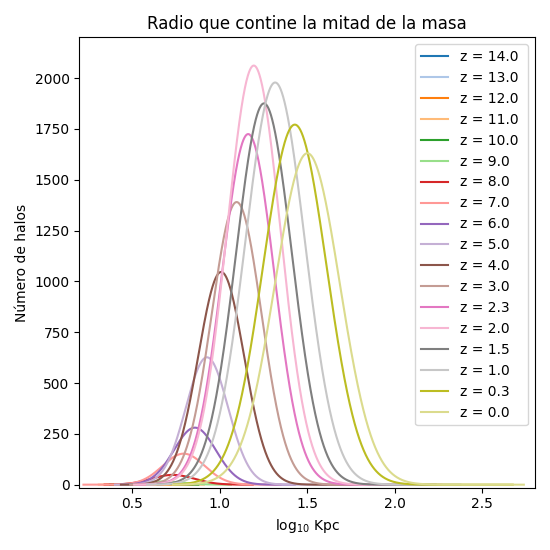
\includegraphics[width = 0.5\linewidth]{RunInvertida/HalfMassRad_Dist_RunInvertida.png}
    \caption[Distribución del Radio que contiene la mitad de la masa]{\footnotesize Comparación de las distribuciones del radio que contiene la mitad de la masa de los halos de materia oscura de un Universo $\Omega_\lambda = 0.309 $, $\Omega_0 = 0.691$.}
    \label{fig:Invertida-HalfMassRadDist}
\end{figure}

\begin{figure}[H]
    \centering
    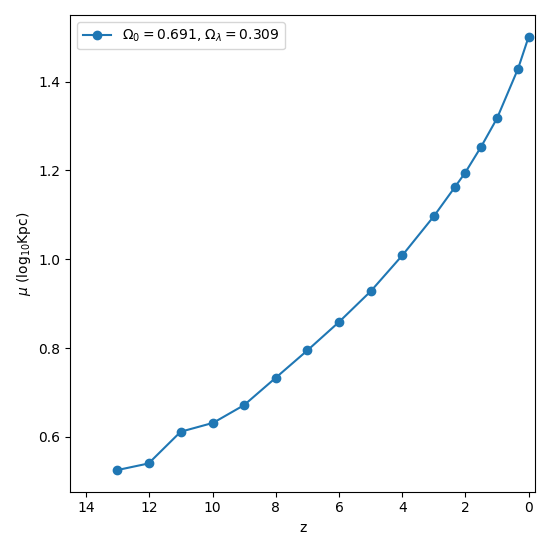
\includegraphics[width = 0.4\linewidth]{RunInvertida/HalfMassRad_Mean_RunInvertida.png}
    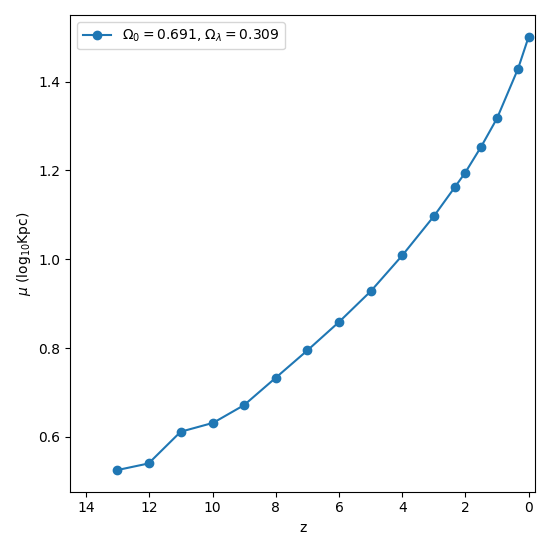
\includegraphics[width = 0.4\linewidth]{RunInvertida/HalfMassRad_Std_RunInvertida.png}
    \caption[Media y desviación estándar del radio de la mitad de la masa]{\footnotesize En la izquierda mostramos la media del radio que contiene la mitad de la masa de los halos de materia oscura y en la derecha se muestra su desviación estándar a lo largo de la evolución del Universo.}
    \label{fig:Invertida-HalfMassRadStats}
\end{figure}

Ahora veamos el comportamiento del radio asociado con la velocidades circular. En las figuras \ref{fig:Invertida-VMaxRadDistSep} y \ref{fig:Invertida-VMaxRadDist} observamos que a lo largo de la evolución de las estructuras tenemos halos con radios que van desde los $2$kpc hasta los $600$kpc. Vemos que la gran mayoría de los halos son halos con tamaños menores a $100$kpc mas al presente y menores a $10$kpc en los redshifts mas altos. En la figura \ref{fig:Invertida-VMaxRadStats} vemos que la media va desde los $4.28$kpc con una desviación de $0.02$kpc en $z=13$ hasta $30.5$kpc con una desviación de $18.7$kpc en $z=0$.

\begin{figure}[H]
    \centering
    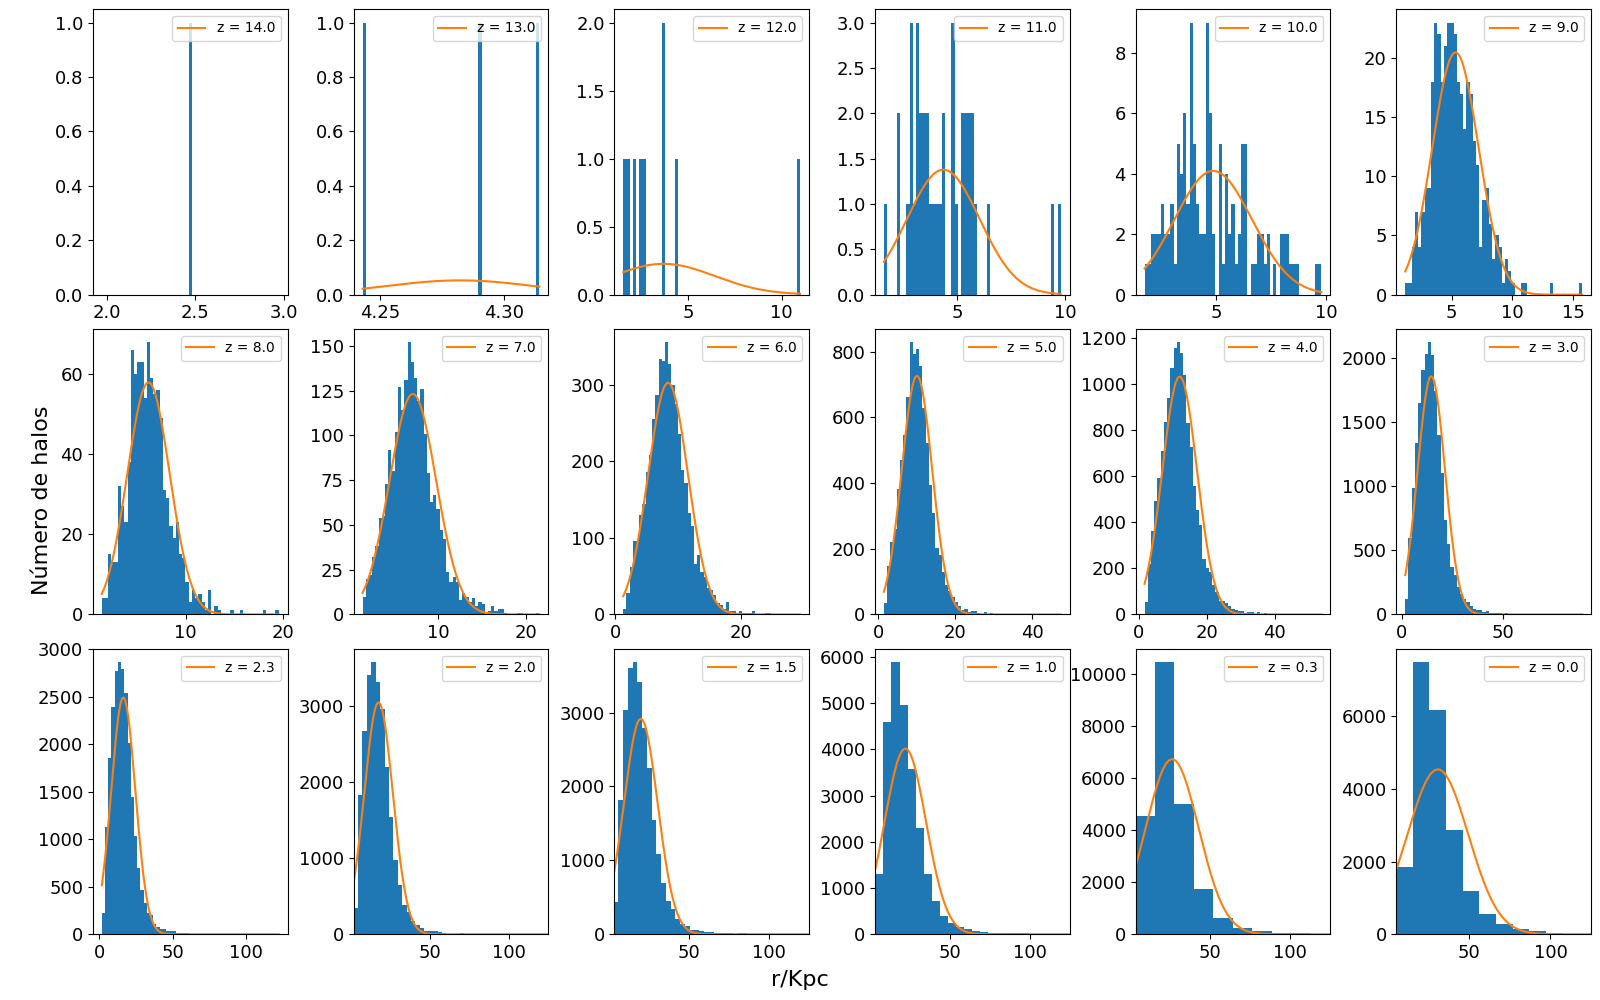
\includegraphics[width = 0.75\linewidth]{RunInvertida/VMaxRad_Dist_RunInvertidaSep.png}
    \caption[Radio donde se alcanza la velocidad máxima radial]{\footnotesize Se muestra el radio donde se alcanza la velocidad máxima radial conforme evoluciona el Universo en una cosmología $\Omega_\lambda = 0.309 $ y $\Omega_0 = 0.691$. Se observa como aumentan la cantidad de halos cada vez mas masivos.}
    \label{fig:Invertida-VMaxRadDistSep}
\end{figure}

\begin{figure}[H]
    \centering
    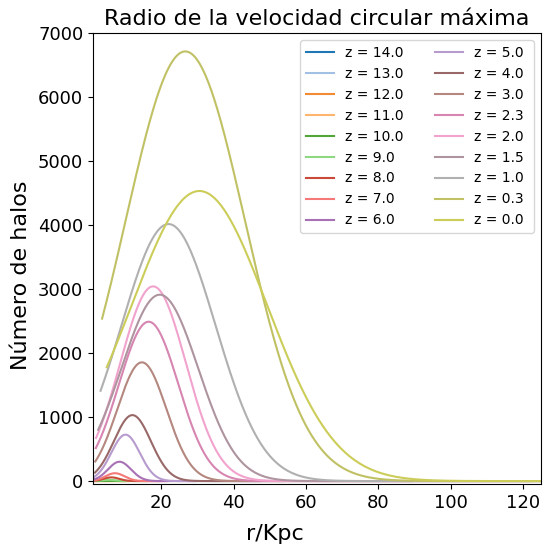
\includegraphics[width = 0.5\linewidth]{RunInvertida/VMaxRad_Dist_RunInvertida.png}
    \caption[Distribución del radio donde se alcanza la velocidad máxima radial]{\footnotesize Comparación de las distribuciones del radio donde se alcanza la velocidad máxima radial de los halos de materia oscura de un Universo $\Omega_\lambda = 0.309 $, $\Omega_0 = 0.691$.}
    \label{fig:Invertida-VMaxRadDist}
\end{figure}

\begin{figure}[H]
    \centering
    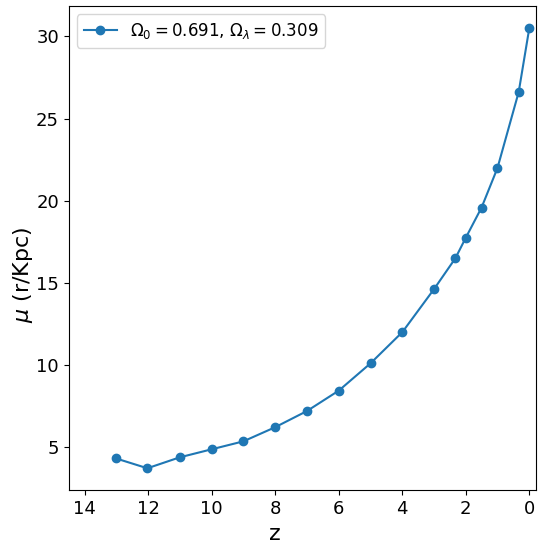
\includegraphics[width = 0.4\linewidth]{RunInvertida/VMaxRad_Mean_RunInvertida.png}
    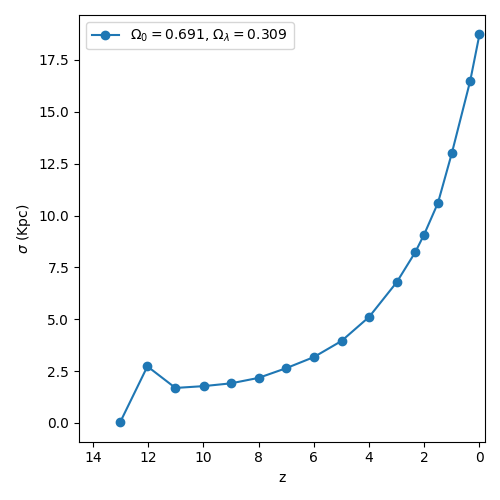
\includegraphics[width = 0.4\linewidth]{RunInvertida/VMaxRad_Std_RunInvertida.png}
    \caption[Media y desviación estándar del Radio donde se alcanza la velocidad máxima radial]{\footnotesize En la izquierda mostramos la media del radio donde se alcanza la velocidad máxima radial de los halos de materia oscura y en la derecha se muestra su desviación estándar a lo largo de la evolución del Universo.}
    \label{fig:Invertida-VMaxRadStats}
\end{figure}

Seguimos con la velocidad circular máxima que se alcanza en estos radios. Podemos apreciar que las velocidades circulares van de los rangos de los $20$km/s hasta los $1400$km/s donde vemos la gran mayoría de los halos en los rangos de $100$km/s y $200$km/s, como se muestra en las figuras \ref{fig:Invertida-VelMaxDistSep} y \ref{fig:Invertida-VelMaxDist}. Lo que podemos ver en la figura \ref{fig:Invertida-VelMaxStats} es que la velocidad  media disminuye rápidamente desde $207.01$km/s con una desviación de $13.71$km/s en $z=13$ hasta que alcanza $106.06$km/s con una desviación de $47.34$km/s en $z=0$. 

\begin{figure}[H]
    \centering
    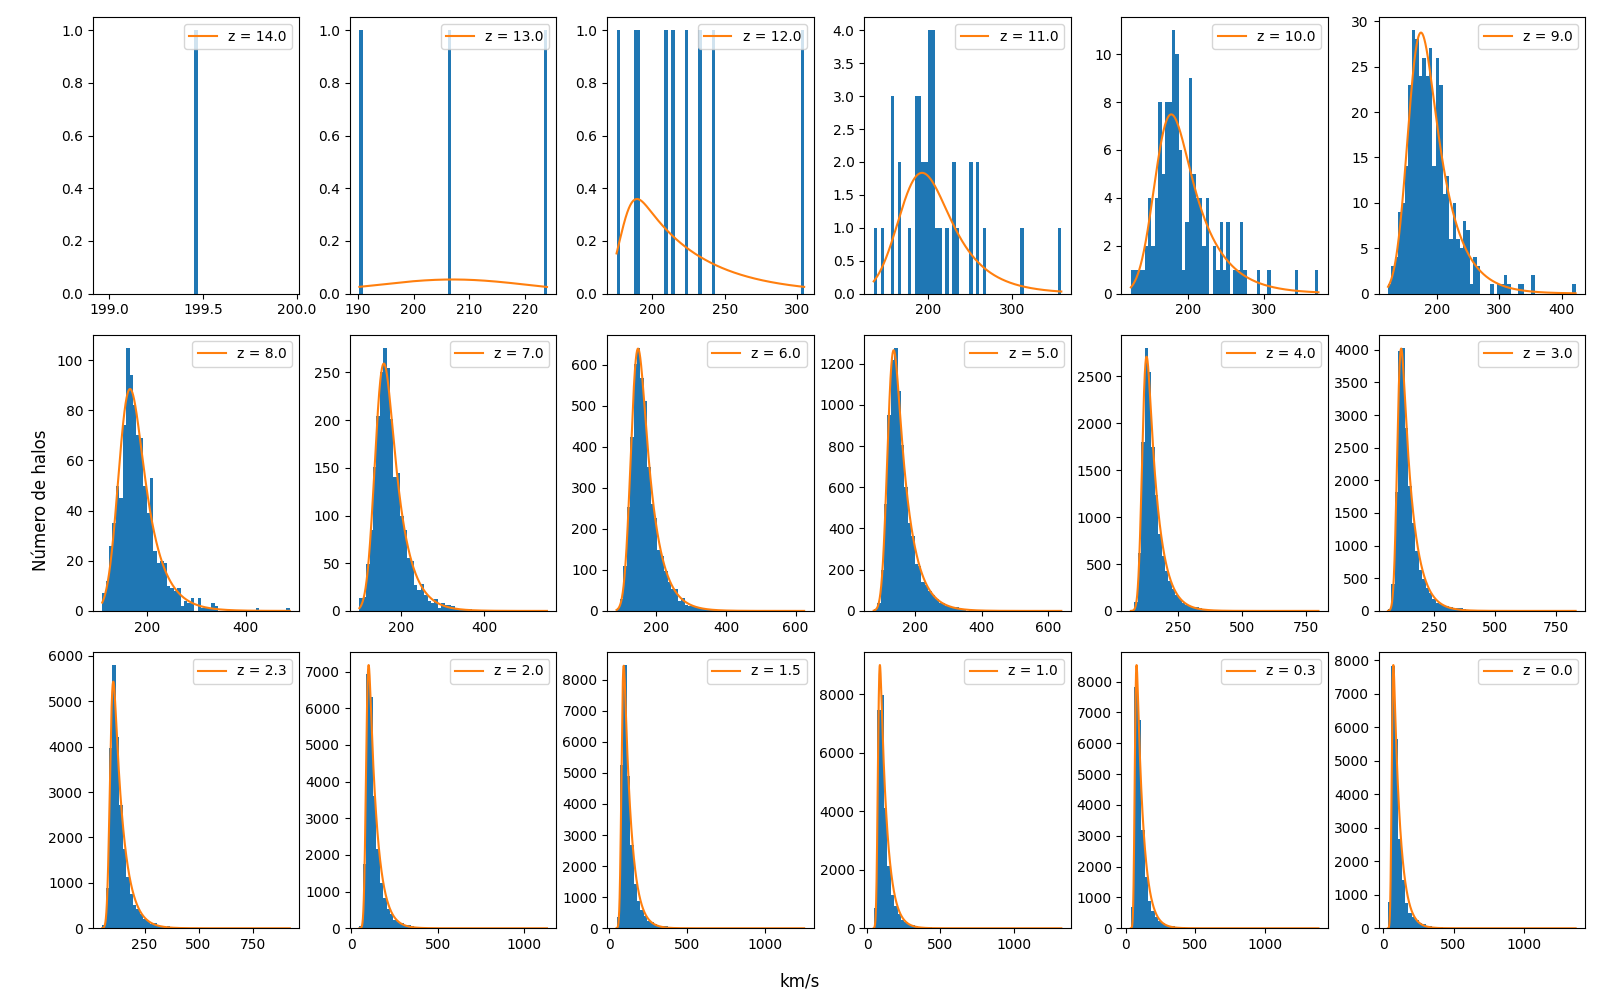
\includegraphics[width = 0.75\linewidth]{RunInvertida/VelMax_Dist_RunInvertidaSep.png}
    \caption[Velocidad circular máxima]{\footnotesize Se muestra la velocidad circular máxima conforme evoluciona el Universo en una cosmología $\Omega_\lambda = 0.309 $ y $\Omega_0 = 0.691$.}
    \label{fig:Invertida-VelMaxDistSep}
\end{figure}

\begin{figure}[H]
    \centering
    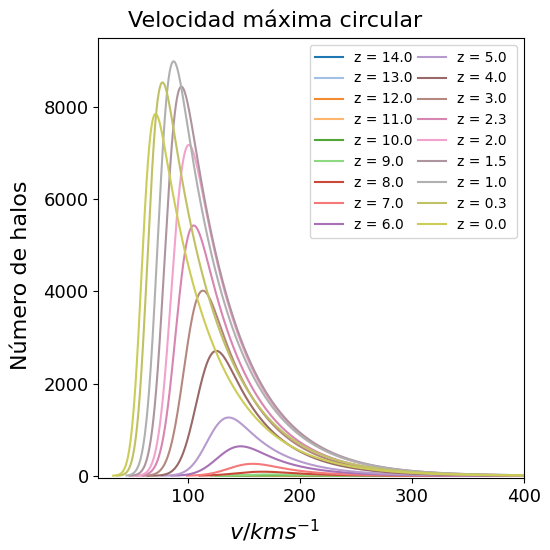
\includegraphics[width = 0.5\linewidth]{RunInvertida/VelMax_Dist_RunInvertida.png}
    \caption[Distribución de la velocidad circular máxima]{\footnotesize Comparación de las distribuciones de la velocidad circular máxima de los halos de materia oscura de un Universo $\Omega_\lambda = 0.309 $, $\Omega_0 = 0.691$.}
    \label{fig:Invertida-VelMaxDist}
\end{figure}

\begin{figure}[H]
    \centering
    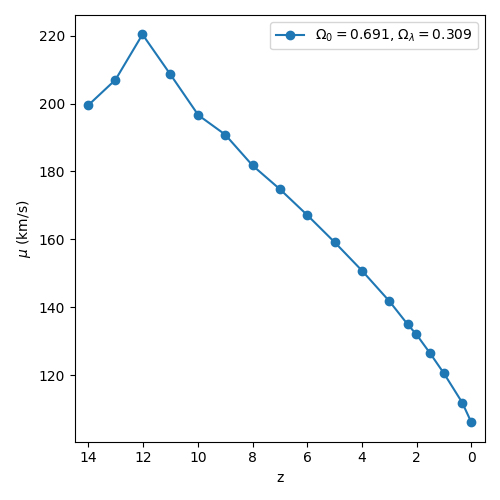
\includegraphics[width = 0.4\linewidth]{RunInvertida/VelMax_Mean_RunInvertida.png}
    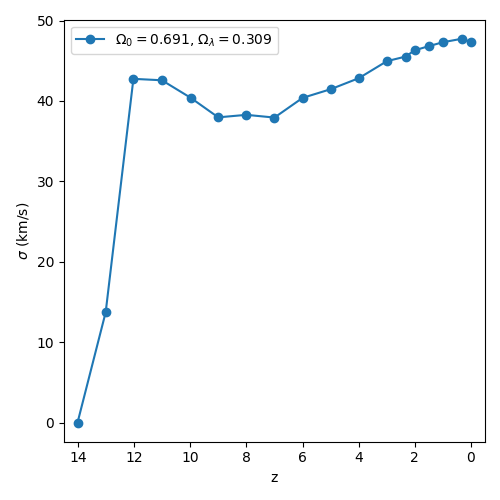
\includegraphics[width = 0.4\linewidth]{RunInvertida/VelMax_Std_RunInvertida.png}
    \caption[Media y desviación estándar de la velocidad circular máxima]{\footnotesize En la izquierda mostramos la media de la velocidad circular máxima de los halos de materia oscura y en la derecha se muestra su desviación estándar a lo largo de la evolución del Universo.}
    \label{fig:Invertida-VelMaxStats}
\end{figure}


La dispersión de velocidades de estos halos esta en los rangos de $17$km/s a los $857$km/s a lo largo de la evolución de los halos. Vemos en las figuras \ref{fig:Invertida-VelDispDistSep} y \ref{fig:Invertida-VelDispDist} que en los $z$ altos vemos que que la mayor parte de los halos se encuentran en el rango de los $100$km/s a los $150$km/s con picos en los $200$km/s y $400$km/s, mientras que en los $z$ bajos vemos los rango que van de $50$km/s y $150$km/s con los picos entre los $400$km/s y $857$km/s. En la figura \ref{fig:Invertida-VelDispStats} observamos que la dispersión de velocidades media disminuye desde los $114.45$km/s con una desviación de $7.96$km/s en $z=14$ a $54.03$km/s con una desviación de $26.70$km/s en $z=0$.


\begin{figure}[H]
    \centering
    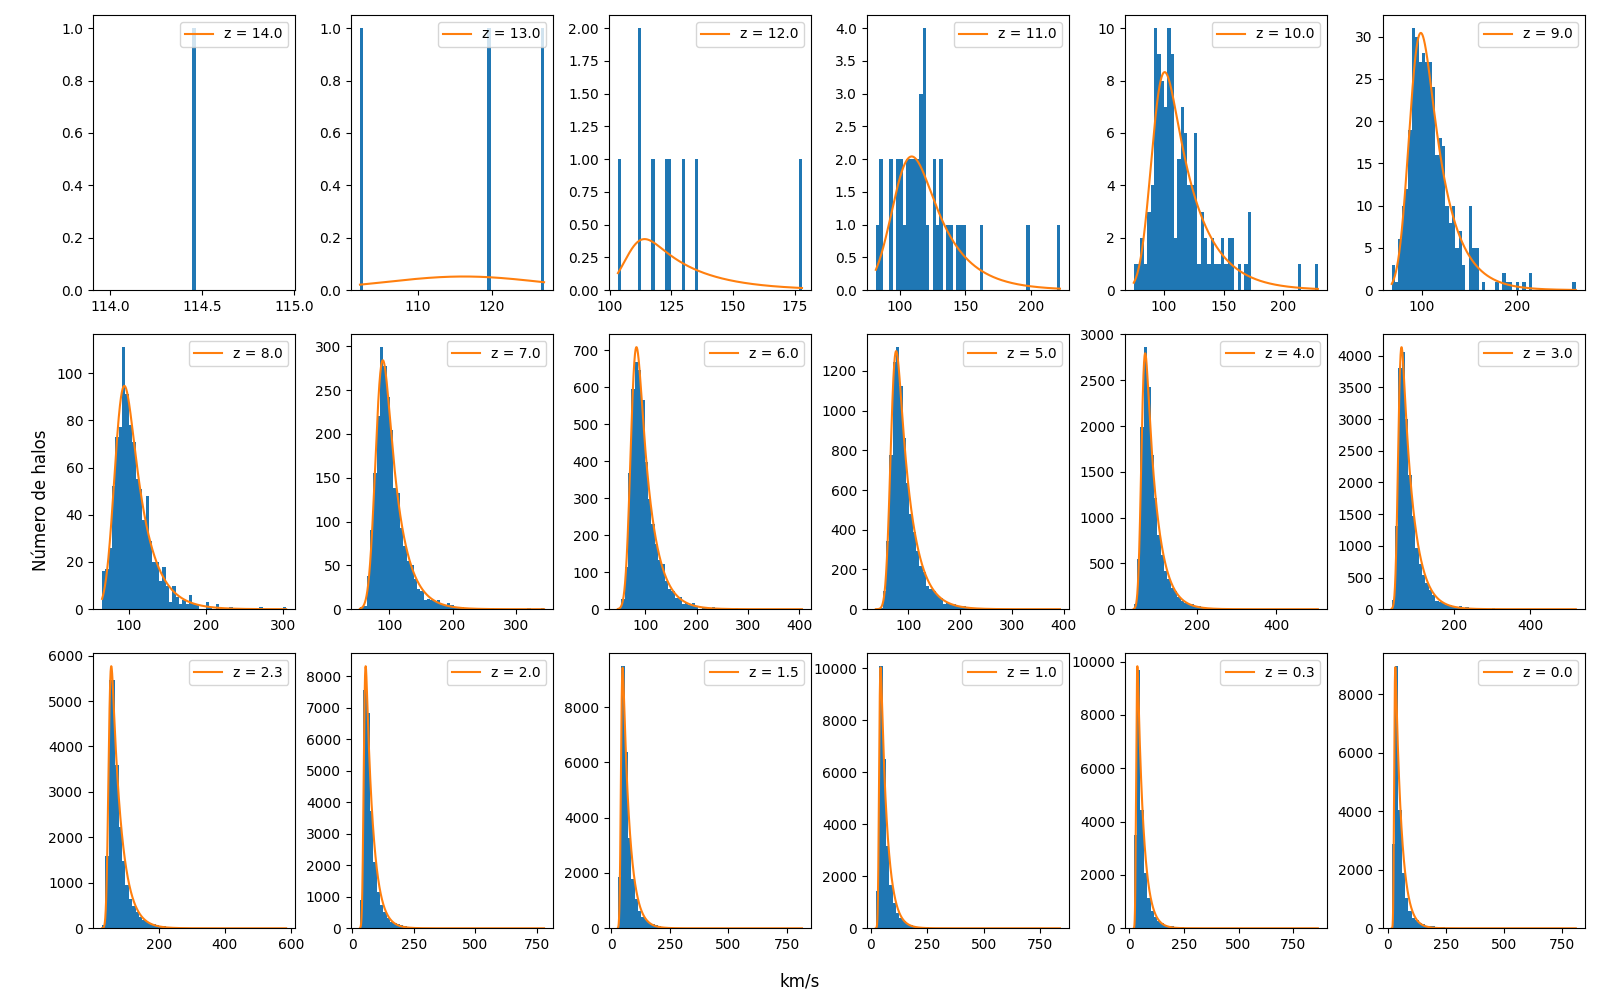
\includegraphics[width = 0.75\linewidth]{RunInvertida/VelDisp_Dist_RunInvertidaSep.png}
    \caption[Dispersión de velocidades]{\footnotesize Se muestra la dispersión de velocidades conforme evoluciona el Universo en una cosmología $\Omega_\lambda = 0.309 $ y $\Omega_0 = 0.691$.}
    \label{fig:Invertida-VelDispDistSep}
\end{figure}

\begin{figure}[H]
    \centering
    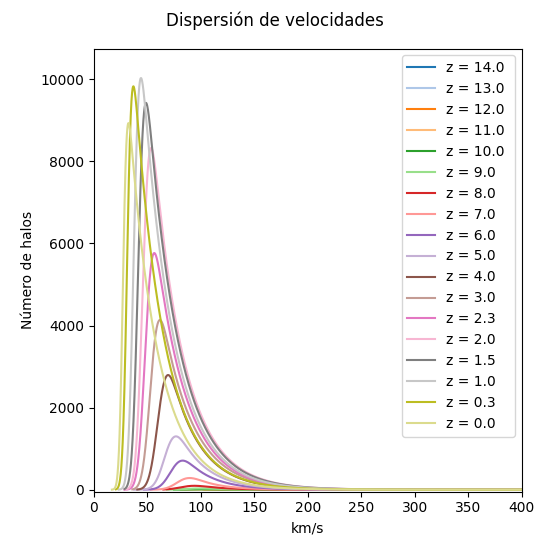
\includegraphics[width = 0.5\linewidth]{RunInvertida/VelDisp_Dist_RunInvertida.png}
    \caption[Distribución de la dispersión de velocidades]{\footnotesize Comparación de las distribuciones de la dispersión de velocidades de los halos de materia oscura de un Universo $\Omega_\lambda = 0.309 $, $\Omega_0 = 0.691$.}
    \label{fig:Invertida-VelDispDist}
\end{figure}

\begin{figure}[H]
    \centering
    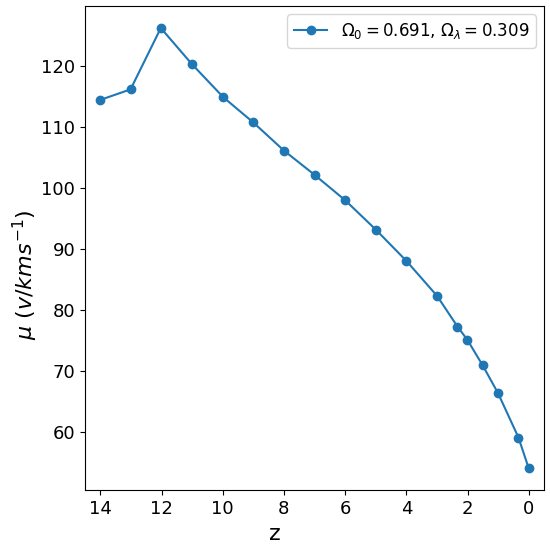
\includegraphics[width = 0.4\linewidth]{RunInvertida/VelDisp_Mean_RunInvertida.png}
    \includegraphics[width = 0.4\linewidth]{RunInvertida/VelDisp_Std_RunInvertida.png}
    \caption[Media y desviación estándar de la dispersión de velocidades]{\footnotesize En la izquierda mostramos la media de la dispersión de velocidades de los halos de materia oscura y en la derecha se muestra su desviación estándar a lo largo de la evolución del Universo.}
    \label{fig:Invertida-VelDispStats}
\end{figure}

La figura \ref{fig:Invertida-DensityMap} muestra la el mapa de densidad de un Universo $\Omega_\lambda = 0.309 $ $\Omega_0 = 0.691$, donde podemos ver la estructura que describimos  en los diferentes puntos de su evolución vista desde un plano .
\begin{figure}[H]
    \centering

    \includegraphics[width = 0.33\linewidth]{RunInvertida/RunInvertidaZ63.png}   %snap 000 z=63
    \includegraphics[width = 0.33\linewidth]{RunInvertida/RunInvertidaZ25.png}   %snap 005 z=25
    \includegraphics[width = 0.32\linewidth]{RunInvertida/RunInvertidaZ20.png}   %snap 010 z=20
    \\
    \includegraphics[width = 0.33\linewidth]{RunInvertida/RunInvertidaZ15.png}   %snap 015 z=15
    \includegraphics[width = 0.33\linewidth]{RunInvertida/RunInvertidaZ10.png}   %snap 020 z=10
    \includegraphics[width = 0.32\linewidth]{RunInvertida/RunInvertidaZ5.png}    %snap 025 z=5
    \\
    \includegraphics[width = 0.33\linewidth]{RunInvertida/RunInvertidaZ3.png}    %snap 027 z=3
    \includegraphics[width = 0.33\linewidth]{RunInvertida/RunInvertidaZ1_5.png}  %snap 030 z=1.5
    \includegraphics[width = 0.32\linewidth]{RunInvertida/RunInvertidaZ0.png}    %snap 033 z=0
    \caption[Mapa de densidad en en diferentes redshift]{ \footnotesize Mapa de densidad de la simulación en diferentes redshifts de una cosmología $\Omega_\lambda = 0.309 $, $\Omega_0 = 0.691$. }
    \label{fig:Invertida-DensityMap}
\end{figure}

%====================================================================================================================
%=====================================  RUN HALF COSMO  =============================================================
%====================================================================================================================
\subsection{Universo con cosmología \texorpdfstring{$\Omega_\lambda = 0.5$, $\Omega_0 = 0.5$ }{Omega lambda = 0.5, Omega 0 = 0.5} }

Hemos visto que como se comporta un Universo con las densidades mas aceptadas y cuando estas se invierten. Ahora veamos un Universo con las densidades iguales ($\Omega_\lambda = 0.5$, $\Omega_0 = 0.5$). Comencemos viendo como se afecta la cantidad de halos. La figura \ref{fig:HalfCosmo-TotalHalos} muestra que los primeros halos aparecen en $z=15$, además muestra que el máximo de halos en las simulaciones que se alcanza fue de $26242$ halos en $z=1.5$. Observamos un comportamiento similar a las cosmologías anteriores donde vemos un crecimiento rápido hasta que alcanza un máximo y después empieza a disminuir.

\begin{figure}[H]
    \centering
    \includegraphics[scale = 0.5]{RunHalfCosmo/TotalHalos_RunHalfCosmo.png}
    \caption[Evolución del número de halos en un Universo $\Omega_\lambda = 0.5 $, $\Omega_0 = 0.5$]{\footnotesize Se muestra el numero de halos y como cambia la cantidad conforme evoluciona el Universo en una cosmología $\Omega_\lambda = 0.5 $ y $\Omega_0 = 0.5$.}    
    \label{fig:HalfCosmo-TotalHalos}
\end{figure}

La distribución de la masa para esta cosmología se observa en las figuras \ref{fig:HalfCosmo-MassDistSep} y \ref{fig:HalfCosmo-MassDist}. Los rangos de la masa se encuentran entre las $10^{10.3}M_\odot$ a $10^{14.5}M_\odot$ a lo largo de de la evolución del sistema. Las primeras estructuras, las que tienen $z$ altos, tenían masas menores a las $10^{12}M_\odot$ y las estructuras en $z$ pequeños la mayor parte de los halos tenían masas entre $10^{10.5}M_\odot$ y $10^{11.5}M_\odot$. Mientras, la figura \ref{fig:HalfCosmo-MassStats} nos muestra el comportamiento medio durante la evolución. Observamos que la masa media incrementa desde $10^{10.65}M_\odot$ con una desviación de $10^{0.1}M_\odot$ en $z=14$ hasta $10^{10.95}M_\odot$ con una desviación de $10^{0.5}M_\odot$ en $z=0$.

\begin{figure}[H]
    \centering
    \includegraphics[width = 0.8\linewidth]{RunHalfCosmo/Mass_Dist_RunHalfCosmoSep.png}
    \caption[Distribución de masa]{\footnotesize Se muestra la distribución de la masa conforme evoluciona el Universo en una cosmología $\Omega_\lambda = 0.5$ y $\Omega_0 = 0.5$. Se observa como aumentan la cantidad de halos cada vez mas masivos.}
    \label{fig:HalfCosmo-MassDistSep}
\end{figure}

\begin{figure}[H]
    \centering
    \includegraphics[width = 0.5\linewidth]{RunHalfCosmo/Mass_Dist_RunHalfCosmo.png}
    \caption[Comparación de distribución de masa Universo]{\footnotesize Comparación de las distribuciones de masa durante la evolución del Universo $\Omega_\lambda = 0.5$, $\Omega_0 = 0.5$. Se observa como crece la cantidad de halos de materia oscura, asi como el tamaño de estos.}
    \label{fig:HalfCosmo-MassDist}
\end{figure}

\begin{figure}[H]
    \centering
    \includegraphics[width = 0.4\linewidth]{RunHalfCosmo/MassMean_RunHalfCosmo.png}
    \includegraphics[width = 0.4\linewidth]{RunHalfCosmo/MassStd_RunHalfCosmo.png}
    \caption[Media y desviación estándar de la distribución de masa]{\footnotesize En la izquierda se muestra la masa media de los halos de materia oscura y se observa como cambia durante la evolución del Universo. En la derecha se muestra la desviación estándar de la masa, la cual nos muestra la variedad que hay de los halos de materia oscura.}
    \label{fig:HalfCosmo-MassStats}
\end{figure}

En las figuras \ref{fig:HalfCosmo-HalfMassRadDistSep} y \ref{fig:HalfCosmo-HalfMassRadDist} podemos ver el radio que contiene la mitad de la masa de los halos a lo largo de la evolución del Universo. Vemos que los radios se encuentran entre los $10^{0.27}$kpc y $10^{2.72}$kpc donde los primeros halos tienen radios entre los $10^{0.29}$kpc y los $10^{1.61}$ y las estructuras mas recientes tienen la mayor parte de los halos en el rango de $10^{1}$kpc y los $10^{1.75}$. El radio medio tiene un crecimiento de $10^{0.53}$kpc con una desviación de $10^{0.09}$kpc en $z=14$ hasta un radio de $10^{1.49}$kpc con una desviación de $10^{0.18}$kpc en $z=0$.

\begin{figure}[H]
    \centering
    \includegraphics[width = 0.75\linewidth]{RunHalfCosmo/HalfMassRad_Dist_RunHalfCosmoSep.png}
    \caption[Radio que contiene la mitad de la masa]{\footnotesize Se muestra el radio que contiene la mitad de la masa conforme evoluciona el Universo en una cosmología $\Omega_\lambda = 0.5 $ y $\Omega_0 = 0.5$.}
    \label{fig:HalfCosmo-HalfMassRadDistSep}
\end{figure}

\begin{figure}[H]
    \centering
    \includegraphics[width = 0.5\linewidth]{RunHalfCosmo/HalfMassRad_Dist_RunHalfCosmo.png}
    \caption[Distribución del Radio que contiene la mitad de la masa]{\footnotesize Comparación de las distribuciones del radio que contiene la mitad de la masa de los halos de materia oscura en un Universo $\Omega_\lambda = 0.5 $ y $\Omega_0 = 0.5$.}
    \label{fig:HalfCosmo-HalfMassRadDist}
\end{figure}

\begin{figure}[H]
    \centering
    \includegraphics[width = 0.4\linewidth]{RunHalfCosmo/HalfMassRad_Mean_RunHalfCosmo.png}
    \includegraphics[width = 0.4\linewidth]{RunHalfCosmo/HalfMassRad_Std_RunHalfCosmo.png}
    \caption[Media y desviación estándar del radio de la mitad de la masa]{\footnotesize En la izquierda mostramos la media del radio que contiene la mitad de la masa de los halos de materia oscura y en la derecha se muestra su desviación estándar a lo largo de la evolución del Universo.}
    \label{fig:HalfCosmo-HalfMassRadStats}
\end{figure}

Ahora veamos el comportamiento del radio asociado con la velocidades circular. En las figuras \ref{fig:HalfCosmo-VMaxRadDistSep} y \ref{fig:HalfCosmo-VMaxRadDist} observamos que a lo largo de la evolución de las estructuras, tenemos halos con radios que van desde los $1$kpc hasta los $590$kpc. Vemos que la gran mayoría de los halos son halos con tamaños menores a $20$kpc mas al presente y menores a $10$kpc en los redshifts mas altos. En la figura \ref{fig:HalfCosmo-VMaxRadStats} vemos que la media va desde los $3.39$kpc con una desviación de $1.18$kpc en $z=13$ hasta $29.44$kpc con una desviación de $17.95$kpc en $z=0$.

\begin{figure}[H]
    \centering
    \includegraphics[width = 0.75\linewidth]{RunHalfCosmo/VMaxRad_Dist_RunHalfCosmoSep.png}
    \caption[Radio donde se alcanza la velocidad máxima radial]{\footnotesize Se muestra el radio donde se alcanza la velocidad máxima radial conforme evoluciona el Universo en una cosmología $\Omega_\lambda = 0.5$ y $\Omega_0 = 0.5$. Se observa como aumentan la cantidad de halos cada vez mas masivos.}
    \label{fig:HalfCosmo-VMaxRadDistSep}
\end{figure}

\begin{figure}[H]
    \centering
    \includegraphics[width = 0.5\linewidth]{RunHalfCosmo/VMaxRad_Dist_RunHalfCosmo.png}
    \caption[Distribución del radio donde se alcanza la velocidad máxima radial]{\footnotesize Comparación de las distribuciones del radio donde se alcanza la velocidad máxima radial de los halos de materia oscura en un Universo $\Omega_\lambda = 0.5$, $\Omega_0 = 0.5$.}
    \label{fig:HalfCosmo-VMaxRadDist}
\end{figure}

\begin{figure}[H]
    \centering
    \includegraphics[width = 0.4\linewidth]{RunHalfCosmo/VMaxRad_Mean_RunHalfCosmo.png}
    \includegraphics[width = 0.4\linewidth]{RunHalfCosmo/VMaxRad_Std_RunHalfCosmo.png}
    \caption[Media y desviación estándar del Radio donde se alcanza la velocidad máxima radial]{\footnotesize En la izquierda mostramos la media del radio donde se alcanza la velocidad máxima radial de los halos de materia oscura y en la derecha se muestra su desviación estándar a lo largo de la evolución del Universo.}
    \label{fig:HalfCosmo-VMaxRadStats}
\end{figure}

Seguimos con la velocidad circular máxima que se alcanza en estos radios. Podemos apreciar que las velocidades circulares van de los rangos de los $25$km/s hasta los $1216$km/s donde vemos la gran mayoría de los halos en los rangos de $30$km/s y $175$km/s, como se muestra en las figuras \ref{fig:HalfCosmo-VelMaxDistSep} y \ref{fig:HalfCosmo-VelMaxDist}. Lo que podemos ver en la figura \ref{fig:HalfCosmo-VelMaxStats} es que la velocidad  media disminuye rápidamente desde $177.53$km/s con una desviación de $2.14$km/s en $z=15$ hasta que alcanza $92.14$km/s con una desviación de $41.30$km/s en $z=0$. 

\begin{figure}[H]
    \centering
    \includegraphics[width = 0.75\linewidth]{RunHalfCosmo/VelMax_Dist_RunHalfCosmoSep.png}
    \caption[Velocidad circular máxima]{\footnotesize Se muestra la velocidad circular máxima conforme evoluciona el Universo en una cosmología $\Omega_\lambda = 0.5 $ y $\Omega_0 = 0.5$.}
    \label{fig:HalfCosmo-VelMaxDistSep}
\end{figure}

\begin{figure}[H]
    \centering
    \includegraphics[width = 0.5\linewidth]{RunHalfCosmo/VelMax_Dist_RunHalfCosmo.png}
    \caption[Distribución de la velocidad circular máxima]{\footnotesize Comparación de las distribuciones de la velocidad circular máxima de los halos de materia oscura en un Universo $\Omega_\lambda = 0.5 $, $\Omega_0 = 0.5$.}
    \label{fig:HalfCosmo-VelMaxDist}
\end{figure}

\begin{figure}[H]
    \centering
    \includegraphics[width = 0.4\linewidth]{RunHalfCosmo/VelMax_Mean_RunHalfCosmo.png}
    \includegraphics[width = 0.4\linewidth]{RunHalfCosmo/VelMax_Std_RunHalfCosmo.png}
    \caption[Media y desviación estándar de la velocidad circular máxima]{\footnotesize En la izquierda mostramos la media de la velocidad circular máxima de los halos de materia oscura y en la derecha se muestra su desviación estándar a lo largo de la evolución del Universo.}
    \label{fig:HalfCosmo-VelMaxStats}
\end{figure}

La dispersión de velocidades de estos halos esta en los rangos de $14$km/s a los $743$km/s a lo largo de la evolución de los halos. Vemos en las figuras \ref{fig:HalfCosmo-VelDispDistSep} y \ref{fig:HalfCosmo-VelDispDist} que en los $z$ altos vemos que que la mayor parte de los halos se encuentran en el rango de los $75$km/s a los $100$km/s con picos en los $347$km/s, mientras que en los $z$ bajos vemos los rango que van de $50$km/s y $80$km/s con los picos entre los $600$km/s y $750$km/s. En la figura \ref{fig:HalfCosmo-VelDispStats} observamos que la dispersión de velocidades media disminuye desde los $100.87$km/s con una desviación de $6.67$km/s en $z=15$ a $46.44$km/s con una desviación de $23.13$km/s en $z=0$.

\begin{figure}[H]
    \centering
    \includegraphics[width = 0.75\linewidth]{RunHalfCosmo/VelDisp_Dist_RunHalfCosmoSep.png}
    \caption[Dispersión de velocidades]{\footnotesize Se muestra la dispersión de velocidades conforme evoluciona el Universo en una cosmología $\Omega_\lambda = 0.5 $ y $\Omega_0 = 0.5$.}
    \label{fig:HalfCosmo-VelDispDistSep}
\end{figure}

\begin{figure}[H]
    \centering
    \includegraphics[width = 0.5\linewidth]{RunHalfCosmo/VelDisp_Dist_RunHalfCosmo.png}
    \caption[Distribución de la dispersión de velocidades]{\footnotesize Comparación de las distribuciones de la dispersión de velocidades de los halos de materia oscura en un Universo $\Omega_\lambda = 0.5 $, $\Omega_0 = 0.5$.}
    \label{fig:HalfCosmo-VelDispDist}
\end{figure}

\begin{figure}[H]
    \centering
    \includegraphics[width = 0.4\linewidth]{RunHalfCosmo/VelDisp_Mean_RunHalfCosmo.png}
    \includegraphics[width = 0.4\linewidth]{RunHalfCosmo/VelDisp_Std_RunHalfCosmo.png}
    \caption[Media y desviación estándar de la dispersión de velocidades]{\footnotesize En la izquierda mostramos la media de la dispersión de velocidades de los halos de materia oscura y en la derecha se muestra su desviación estándar a lo largo de la evolución del Universo.}
    \label{fig:HalfCosmo-VelDispStats}
\end{figure}

La figura \ref{fig:HalfCosmo-DensityMap} muestra la el mapa de densidad de un Universo $\Omega_\lambda = 0.5 $ $\Omega_0 = 0.5$, donde podemos ver la estructura que describimos  en los diferentes puntos de su evolución vista desde un plano .
\begin{figure}[H]
    \centering

    \includegraphics[width = 0.33\linewidth]{RunHalfCosmo/RunHalfCosmoZ63.png}   %snap 000 z=63
    \includegraphics[width = 0.33\linewidth]{RunHalfCosmo/RunHalfCosmoZ25.png}   %snap 005 z=25
    \includegraphics[width = 0.32\linewidth]{RunHalfCosmo/RunHalfCosmoZ20.png}   %snap 010 z=20
    \\
    \includegraphics[width = 0.33\linewidth]{RunHalfCosmo/RunHalfCosmoZ15.png}   %snap 015 z=15
    \includegraphics[width = 0.33\linewidth]{RunHalfCosmo/RunHalfCosmoZ10.png}   %snap 020 z=10
    \includegraphics[width = 0.32\linewidth]{RunHalfCosmo/RunHalfCosmoZ5.png}    %snap 025 z=5
    \\
    \includegraphics[width = 0.33\linewidth]{RunHalfCosmo/RunHalfCosmoZ3.png}    %snap 027 z=3
    \includegraphics[width = 0.33\linewidth]{RunHalfCosmo/RunHalfCosmoZ1_5.png}  %snap 030 z=1.5
    \includegraphics[width = 0.32\linewidth]{RunHalfCosmo/RunHalfCosmoZ0.png}    %snap 033 z=0
    \caption[Mapa de densidad en en diferentes redshift]{ \footnotesize Mapa de densidad de la simulación en diferentes redshifts de una cosmología $\Omega_\lambda = 0.5 $, $\Omega_0 = 0.5$. }
    \label{fig:HalfCosmo-DensityMap}
\end{figure}

%====================================================================================================================
%=====================================  Run Sub-Crítica  ============================================================
%====================================================================================================================
\section[Cosmología Sub-Crítica \texorpdfstring{$\Omega < 1$}{Omega < 1}]{Cosmología Sub-Crítica \texorpdfstring{$\Omega < 1$}{Omega < 1}}

\noindent Hemos visto los efectos en un Universo plano, ahora veamos tres nuevas cosmologías pero ahora son Universos abiertos acelerados, o bien un Universo Sub-Crítico. Estas nuevas cosmologías se eligieron de manera de obtener una idea de los efectos en el Universo cuando se altera una de sus densidad como se realizo anteriormente. Empezando con una cosmología donde las densidades son $\Omega_\lambda = 0$, $\Omega_0 = 0.309$, en este universo veremos los efectos de un Universo sin presencia de energía oscura. Luego pasaremos nuestra atención a estudiar los efectos de un Universo donde quitamos la mitad de la densidad de energía ($\Omega_\lambda = 0.3455$, $\Omega_0 = 0.309$) y para terminar con las cosmologías sub-críticas veremos los efectos en un Universo donde consideramos la mitad de la densidad de materia ($\Omega_\lambda = 0.5$, $\Omega_0 = 0.5$).

%====================================================================================================================
%====================================  Run No Dark Energy ===========================================================
%====================================================================================================================

\subsection{Universo con cosmología \texorpdfstring{$\Omega_\lambda = 0$, $\Omega_0 = 0.309$ }{Omega lambda = 0, Omega 0 = 0.309}  }

La primera cosmología es en la que no hay efectos de la energía oscura. Lo primero que podemos observar en la figura \ref{fig:NoDE_TotalHalos} es que las estructuras se empiezan a formar a partir del redshift $z=25$. En $z= 2.33$ es donde alcanzamos la mayor cantidad halos. Alrededor de $z = 16$ es cuando empezamos a ver un crecimiento apreciable en la cantidad de halos.

\begin{figure}[H]
    \centering
    \includegraphics[scale = 0.5]{RunNoDE/TotalHalos_RunNoDE.png}
    \caption[Evolución del número de halos en un Universo $\Omega_\lambda = 0$, $\Omega_0 = 0.309$]{\footnotesize Se muestra el numero de halos según el redshift y podemos observar como evoluciona el Universo en una cosmología $\Omega_\lambda = 0$ y $\Omega_0 = 0.309$.}
    \label{fig:NoDE_TotalHalos}
\end{figure}

La distribución de la masa para esta cosmología se observa en las figuras \ref{fig:NoDE-MassDistSep} y \ref{fig:NoDE-MassDist}. Los rangos de la masa se encuentran entre las $10^{10.31}M_\odot$ a $10^{14.35}M_\odot$ a lo largo de de la evolución del sistema. Las primeras estructuras, las que tienen $z$ altos, tenían masas menores a las $10^{11}M_\odot$ y las estructuras en $z$ pequeños la mayor parte de los halos tenían masas entre $10^{9.8}M_\odot$ y $10^{11}M_\odot$ con estructuras que alcanzan $10^{14.03}M_\odot$. Mientras, la figura \ref{fig:NoDE-MassStats} nos muestra el comportamiento medio durante la evolución donde observamos que la masa media incrementa desde $10^{10.42}M_\odot$ con una desviación de $10^{0.11}M_\odot$ en $z=25$ hasta $10^{10.76}M_\odot$ con una desviación de $10^{0.49}M_\odot$ en $z=0$.

\begin{figure}[H]
    \centering
    \includegraphics[width = 0.8\linewidth]{RunNoDE/Mass_Dist_RunNoDESep.png}
    \caption[Distribución de masa]{\footnotesize Tenemos la cantidad de halos en diferentes rangos de masa. Se muestran la distribución de la masa conforme evoluciona el Universo en una cosmología $\Omega_\lambda = 0$ y $\Omega_0 = 0.309$. Se tienen las distribuciones en los diferentes redshifts empezando en $z=25$ en la parte superior izquierda y terminado en $z=0$ en la parte inferior derecha. Se observa como aumentan la cantidad de halos cada vez mas masivos.}
    \label{fig:NoDE-MassDistSep}
\end{figure}

\begin{figure}[H]
    \centering
    \includegraphics[width = 0.5\linewidth]{RunNoDE/Mass_Dist_RunNoDE.png}
    \caption[Comparación de distribución de masa]{\footnotesize Tenemos la cantidad de halos en los diferentes rangos de masa. Comparamos de las distribuciones de masa durante la evolución del Universo $\Omega_\lambda = 0$, $\Omega_0 = 0.309$. Se muestra la cantidad de halos en un rango de masas. Se observa como crece la cantidad de halos de materia oscura, asi como el tamaño de estos.}
    \label{fig:NoDE-MassDist}
\end{figure}

\begin{figure}[H]
    \centering
    \includegraphics[width = 0.4\linewidth]{RunNoDE/MassMean_RunNoDE.png}
    \includegraphics[width = 0.4\linewidth]{RunNoDE/MassStd_RunNoDE.png}
    \caption[Media y desviación estándar de la distribución de masa]{\footnotesize En la izquierda se muestra la masa media de los halos de materia oscura y se observa como cambia durante la evolución del Universo. En la derecha se muestra la desviación estándar de la masa, la cual nos muestra la variedad que hay de los halos de materia oscura.}
    \label{fig:NoDE-MassStats}
\end{figure}

En las figuras \ref{fig:NoDE-HalfMassRadDistSep} y \ref{fig:NoDE-HalfMassRadDist} podemos ver el radio que contiene la mitad de la masa de los halos a lo largo de la evolución del Universo. Vemos que los radios se encuentran entre los $10^{0.09}$kpc y $10^{2.57}$kpc donde los primeros halos tienen radios entre los $10^{0.09}$kpc y los $10^{0.65}$ y las estructuras mas recientes tienen la mayor parte de los halos en el rango de $10^{1}$kpc y los $10^{1.75}$kpc con halos que alcanzan hasta los $10^{2.57}kpc$. En la figura \ref{fig:NoDE-HalfMassRadStats} vemos el crecimiento del radio medio desde $10^{0.32}$kpc con una desviación de $10^{0.12}$kpc en $z=25$ hasta un radio de $10^{1.39}$kpc con una desviación de $10^{0.18}$kpc en $z=0$. También vemos que en la desviación estándar hay mucha variedad en los primeros $z$ pero mas al presente vemos crecimiento mas estable.

\begin{figure}[H]
    \centering
    \includegraphics[width = 0.75\linewidth]{RunNoDE/HalfMassRad_Dist_RunNoDESep.png}
    \caption[Radio que contiene la mitad de la masa]{\footnotesize Se muestra la cantidad de halos que tiene el radio que contiene la mitad de la masa conforme evoluciona el Universo en una cosmología $\Omega_\lambda = 0$ y $\Omega_0 = 0.309$. Se tienen las distribuciones en los diferentes redshifts empezando en $z=25$ en la parte superior izquierda y terminado en $z=0$ en la parte inferior derecha.}
    \label{fig:NoDE-HalfMassRadDistSep}
\end{figure}

\begin{figure}[H]
    \centering
    \includegraphics[width = 0.5\linewidth]{RunNoDE/HalfMassRad_Dist_RunNoDE.png}
    \caption[Distribución del radio que contiene la mitad de la masa]{\footnotesize Mostramos la cantidad de halos de materia oscura que tienen un radio que contiene la mitad de la masa en un Universo $\Omega_\lambda = 0$, $\Omega_0 = 0.309$.}
    \label{fig:NoDE-HalfMassRadDist}
\end{figure}

\begin{figure}[H]
    \centering
    \includegraphics[width = 0.4\linewidth]{RunNoDE/HalfMassRad_Mean_RunNoDE.png}
    \includegraphics[width = 0.4\linewidth]{RunNoDE/HalfMassRad_Std_RunNoDE.png}
    \caption[Media y desviación estándar del radio de la mitad de la masa]{\footnotesize En la izquierda mostramos la media del radio que contiene la mitad de la masa de los halos de materia oscura y en la derecha se muestra su desviación estándar a lo largo de la evolución del Universo, desde un $z=25$ hasta un $z=0$.}
    \label{fig:NoDE-HalfMassRadStats}
\end{figure}

En las figuras \ref{fig:NoDE-VMaxRadDistSep} y \ref{fig:NoDE-VMaxRadDist} observamos que a lo largo de la evolución de las estructuras, tenemos halos con radios que van desde los $0.66$kpc hasta los $271.91$kpc. Vemos que la gran mayoría de los halos son halos con tamaños menores a $40$kpc con halos que alcanzan hasta los $271.91$kpc mas al presente y menores a $6$kpc con estructuras que alcanzan $6.16$kpc en los redshifts mas altos. En la figura \ref{fig:NoDE-VMaxRadStats} vemos que la media va desde los $1.76$kpc con una desviación de $0.40$kpc en $z=25$ hasta $21.99$kpc con una desviación de $10.78$kpc en $z=0$.

\begin{figure}[H]
    \centering
    \includegraphics[width = 0.75\linewidth]{RunNoDE/VMaxRad_Dist_RunNoDESep.png}
    \caption[Radio donde se alcanza la velocidad máxima radial]{\footnotesize Se muestra el radio donde se alcanza la velocidad máxima radial conforme evoluciona el Universo en una cosmología $\Omega_\lambda = 0$ y $\Omega_0 = 0.309$. Se tienen las distribuciones en los diferentes redshifts empezando en $z=25$ en la parte superior izquierda y terminado en $z=0$ en la parte inferior derecha.}
    \label{fig:NoDE-VMaxRadDistSep}
\end{figure}

\begin{figure}[H]
    \centering
    \includegraphics[width = 0.5\linewidth]{RunNoDE/VMaxRad_Dist_RunNoDE.png}
    \caption[Distribución del radio donde se alcanza la velocidad máxima radial]{\footnotesize Se muestra la cantidad de halos de materia oscura con el radio donde se alcanza la velocidad máxima radial en un Universo $\Omega_\lambda = 0$, $\Omega_0 = 0.309$.}
    \label{fig:NoDE-VMaxRadDist}
\end{figure}

\begin{figure}[H]
    \centering
    \includegraphics[width = 0.4\linewidth]{RunNoDE/VMaxRad_Mean_RunNoDE.png}
    \includegraphics[width = 0.4\linewidth]{RunNoDE/VMaxRad_Std_RunNoDE.png}
    \caption[Media y desviación estándar del Radio donde se alcanza la velocidad máxima radial]{\footnotesize En la izquierda mostramos la media del radio donde se alcanza la velocidad máxima radial de los halos de materia oscura y en la derecha se muestra su desviación estándar a lo largo de la evolución del Universo, desde un $z=25$ hasta un $z=0$.}
    \label{fig:NoDE-VMaxRadStats}
\end{figure}


Pasando a las velocidades, podemos apreciar que las velocidades circulares van de los rangos de los $23.99$km/s hasta los $1167.42$km/s donde vemos la gran mayoría de los halos en los rangos de $125$km/s y $175$km/s para los $z$ altos y entre los $50$km/s y $100$km/s mas al presente, como se muestra en las figuras \ref{fig:NoDE-VelMaxDistSep} y \ref{fig:NoDE-VelMaxDist}. Lo que podemos ver en la figura \ref{fig:NoDE-VelMaxStats} es que la velocidad media disminuye rápidamente desde $178.18$km/s con una desviación de $29.43$km/s en $z=25$ hasta que alcanza $82.60$km/s con una desviación de $38.29$km/s en $z=0$.

\begin{figure}[H]
    \centering
    \includegraphics[width = 0.75\linewidth]{RunNoDE/VelMax_Dist_RunNoDESep.png}
    \caption[Velocidad circular máxima]{\footnotesize Se muestra la velocidad circular máxima conforme evoluciona el Universo en una cosmología $\Omega_\lambda = 0$ y $\Omega_0 = 0.309$. Se tienen las distribuciones en los diferentes redshifts empezando en $z=25$ en la parte superior izquierda y terminado en $z=0$ en la parte inferior derecha.}
    \label{fig:NoDE-VelMaxDistSep}
\end{figure}

\begin{figure}[H]
    \centering
    \includegraphics[width = 0.5\linewidth]{RunNoDE/VelMax_Dist_RunNoDE.png}
    \caption[Distribución de la velocidad circular máxima]{\footnotesize Mostramos la cantidad de halos de materia oscura en los diferentes rangos de velocidad circular máxima en un Universo $\Omega_\lambda = 0$, $\Omega_0 = 0.309$.}
    \label{fig:NoDE-VelMaxDist}
\end{figure}

\begin{figure}[H]
    \centering
    \includegraphics[width = 0.4\linewidth]{RunNoDE/VelMax_Mean_RunNoDE.png}
    \includegraphics[width = 0.4\linewidth]{RunNoDE/VelMax_Std_RunNoDE.png}
    \caption[Media y desviación estándar de la velocidad circular máxima]{\footnotesize En la izquierda mostramos la media de la velocidad circular máxima de los halos de materia oscura y en la derecha se muestra su desviación estándar a lo largo de la evolución del Universo, desde un $z=25$ hasta un $z=0$.}
    \label{fig:NoDE-VelMaxStats}
\end{figure}

Continuemos con la dispersion de las velocidades de los halos de materia oscura. La dispersión de velocidades de estos halos esta en los rangos de $12.66$km/s a los $711.39$km/s a lo largo de la evolución de los halos. Vemos en las figuras \ref{fig:NoDE-VelDispDistSep} y \ref{fig:NoDE-VelDispDist} que en los $z$ altos vemos que que la mayor parte de los halos se encuentran en el rango de los $80$km/s a los $110$km/s con picos en los $217.65$km/s, mientras que en los $z$ bajos vemos los rango que van de $20$km/s y $50$km/s con los picos en los $658.36$km/s. En la figura \ref{fig:NoDE-VelDispStats} observamos que la dispersión de velocidades media disminuye desde los $101.07$km/s con una desviación de $14.75$km/s en $z=25$ a $39.01$km/s con una desviación de $20.08$km/s en $z=0$.

\begin{figure}[H]
    \centering
    \includegraphics[width = 0.75\linewidth]{RunNoDE/VelDisp_Dist_RunNoDESep.png}
    \caption[Dispersión de velocidades]{\footnotesize Se muestra la dispersión de velocidades conforme evoluciona el Universo en una cosmología $\Omega_\lambda = 0$ y $\Omega_0 = 0.309$.Se tienen las distribuciones en los diferentes redshifts empezando en $z=17$ en la parte superior izquierda y terminado en $z=0$ en la parte inferior derecha.}
    \label{fig:NoDE-VelDispDistSep}
\end{figure}

\begin{figure}[H]
    \centering
    \includegraphics[width = 0.5\linewidth]{RunNoDE/VelDisp_Dist_RunNoDE.png}
    \caption[Distribución de la dispersión de velocidades]{\footnotesize Mostramos la dispersion de velocidades de los halos de materia oscura en un Universo $\Omega_\lambda = 0$, $\Omega_0 = 0.309$.}
    \label{fig:NoDE-VelDispDist}
\end{figure}

\begin{figure}[H]
    \centering
    \includegraphics[width = 0.4\linewidth]{RunNoDE/VelDisp_Mean_RunNoDE.png}
    \includegraphics[width = 0.4\linewidth]{RunNoDE/VelDisp_Std_RunNoDE.png}
    \caption[Media y desviación estándar de la dispersión de velocidades]{\footnotesize En la izquierda mostramos la media de la dispersión de velocidades de los halos de materia oscura y en la derecha se muestra su desviación estándar a lo largo de la evolución del Universo.}
    \label{fig:NoDE-VelDispStats}
\end{figure}

La figura \ref{fig:NoDE-DensityMap} muestra la el mapa de densidad de un Universo $\Omega_\lambda = 0$ $\Omega_0 = 0.309$, donde podemos ver la estructura que describimos  en los diferentes puntos de su evolución vista desde un plano .
\begin{figure}[H]
    \centering

    \includegraphics[width = 0.33\linewidth]{RunNoDE/RunNoDEZ63.png}   %snap 000 z=63
    \includegraphics[width = 0.33\linewidth]{RunNoDE/RunNoDEZ25.png}   %snap 005 z=25
    \includegraphics[width = 0.32\linewidth]{RunNoDE/RunNoDEZ20.png}   %snap 010 z=20
    \\
    \includegraphics[width = 0.33\linewidth]{RunNoDE/RunNoDEZ15.png}   %snap 015 z=15
    \includegraphics[width = 0.33\linewidth]{RunNoDE/RunNoDEZ10.png}   %snap 020 z=10
    \includegraphics[width = 0.32\linewidth]{RunNoDE/RunNoDEZ5.png}    %snap 025 z=5
    \\
    \includegraphics[width = 0.33\linewidth]{RunNoDE/RunNoDEZ3.png}    %snap 027 z=3
    \includegraphics[width = 0.33\linewidth]{RunNoDE/RunNoDEZ1_5.png}  %snap 030 z=1.5
    \includegraphics[width = 0.32\linewidth]{RunNoDE/RunNoDEZ0.png}    %snap 033 z=0
    \caption[Mapa de densidad en en diferentes redshift]{ \footnotesize Mapa de densidad de la simulación en diferentes redshifts de una cosmología $\Omega_\lambda = 0$, $\Omega_0 = 0.309$. }
    \label{fig:NoDE-DensityMap}
\end{figure}

%====================================================================================================================
%=======================================  Run Low Omega_0 ===========================================================
%====================================================================================================================

\subsection{Universo con cosmología \texorpdfstring{$\Omega_\lambda = 0.691$, $\Omega_0 = 0.1545$ }{Omega lambda = 0.691, Omega 0 = 0.1545}  }

Hemos visto los efectos de la ausencia de energía oscura, ahora veremos loes efectos de una disminución de la densidad de materia. Lo primero que podemos observar en la figura \ref{fig:Low0_TotalHalos} es que las estructuras se empiezan a formar a partir del redshift $z=22$, igual que cuando  hay una ausencia de energía oscura. En $z= 2.33$ es donde alcanzamos la mayor cantidad halos a lo largo de la evolución del Universo. Alrededor de $z = 14$ es cuando empezamos a ver un crecimiento apreciable en la cantidad de halos.

\begin{figure}[H]
    \centering
    \includegraphics[scale = 0.5]{RunLow0/TotalHalos_RunLow0.png}
    \caption[Evolución del número de halos en un Universo $\Omega_\lambda = 0.691$, $\Omega_0 = 0.1545$]{\footnotesize Se muestra el numero de halos según el redshift y podemos observar como evoluciona el Universo en una cosmología $\Omega_\lambda = 0.691 $ y $\Omega_0 = 0.1545$.}
    \label{fig:Low0_TotalHalos}
\end{figure}

La distribución de la masa para esta cosmología se observa en las figuras \ref{fig:Low0-MassDistSep} y \ref{fig:Low0-MassDist}. Los rangos de la masa se encuentran entre las $10^{9.81}M_\odot$ a $10^{14.03}M_\odot$ a lo largo de de la evolución del sistema. Las primeras estructuras, las que tienen $z$ altos, tenían masas menores a las $10^{11.5}M_\odot$ y las estructuras en $z$ pequeños la mayor parte de los halos tenían masas entre $10^{10.5}M_\odot$ y $10^{11}M_\odot$ con estructuras que alcanzan $10^{14.32}M_\odot$. Mientras, la figura \ref{fig:Low0-MassStats} nos muestra el comportamiento medio durante la evolución donde observamos que la masa media incrementa desde $10^{10.14}M_\odot$ con una desviación de $10^{0.11}M_\odot$ en $z=23$ hasta $10^{10.45}M_\odot$ con una desviación de $10^{0.50}M_\odot$ en $z=0$.

\begin{figure}[H]
    \centering
    \includegraphics[width = 0.8\linewidth]{RunLow0/Mass_Dist_RunLow0Sep.png}
    \caption[Distribución de masa]{\footnotesize Tenemos la cantidad de halos en diferentes rangos de masa. Se muestran la distribución de la masa conforme evoluciona el Universo en una cosmología $\Omega_\lambda = 0.691$ y $\Omega_0 = 0.1545$. Se tienen las distribuciones en los diferentes redshifts empezando en $z=22$ en la parte superior izquierda y terminado en $z=0$ en la parte inferior derecha. Se observa como aumentan la cantidad de halos cada vez mas masivos.}
    \label{fig:Low0-MassDistSep}
\end{figure}

\begin{figure}[H]
    \centering
    \includegraphics[width = 0.5\linewidth]{RunLow0/Mass_Dist_RunLow0.png}
    \caption[Comparación de distribución de masa]{\footnotesize Tenemos la cantidad de halos en los diferentes rangos de masa. Comparamos de las distribuciones de masa durante la evolución del Universo $\Omega_\lambda = 0.691$, $\Omega_0 = 0.1545$. Se muestra la cantidad de halos en un rango de masas. Se observa como crece la cantidad de halos de materia oscura, asi como el tamaño de estos.}
    \label{fig:Low0-MassDist}
\end{figure}

\begin{figure}[H]
    \centering
    \includegraphics[width = 0.4\linewidth]{RunLow0/MassMean_RunLow0.png}
    \includegraphics[width = 0.4\linewidth]{RunLow0/MassStd_RunLow0.png}
    \caption[Media y desviación estándar de la distribución de masa]{\footnotesize En la izquierda se muestra la masa media de los halos de materia oscura y se observa como cambia durante la evolución del Universo. En la derecha se muestra la desviación estándar de la masa, la cual nos muestra la variedad que hay de los halos de materia oscura.}
    \label{fig:Low0-MassStats}
\end{figure}

En las figuras \ref{fig:Low0-HalfMassRadDistSep} y \ref{fig:Low0-HalfMassRadDist} podemos ver el radio que contiene la mitad de la masa de los halos a lo largo de la evolución del Universo. Vemos que los radios se encuentran entre los $10^{0.08}$kpc y $10^{2.59}$kpc donde los primeros halos tienen radios entre los $10^{0.08}$kpc y los $10^{0.75}$ y las estructuras mas recientes tienen la mayor parte de los halos en el rango de $10^{1.08}$kpc y los $10^{1.60}$kpc con halos que alcanzan hasta los $10^{2.59}kpc$. En la figura \ref{fig:Low0-HalfMassRadStats} vemos el crecimiento del radio medio desde $10^{0.46}$kpc con una desviación de $10^{0.04}$kpc en $z=23$ hasta un radio de $10^{1.40}$kpc con una desviación de $10^{0.18}$kpc en $z=0$.

\begin{figure}[H]
    \centering
    \includegraphics[width = 0.75\linewidth]{RunLow0/HalfMassRad_Dist_RunLow0Sep.png}
    \caption[Radio que contiene la mitad de la masa]{\footnotesize Se muestra la cantidad de halos que tiene el radio que contiene la mitad de la masa conforme evoluciona el Universo en una cosmología $\Omega_\lambda = 0.691$ y $\Omega_0 = 0.1545$. Se tienen las distribuciones en los diferentes redshifts empezando en $z=25$ en la parte superior izquierda y terminado en $z=0$ en la parte inferior derecha.}
    \label{fig:Low0-HalfMassRadDistSep}
\end{figure}

\begin{figure}[H]
    \centering
    \includegraphics[width = 0.5\linewidth]{RunLow0/HalfMassRad_Dist_RunLow0.png}
    \caption[Distribución del radio que contiene la mitad de la masa]{\footnotesize Mostramos la cantidad de halos de materia oscura que tienen un radio que contiene la mitad de la masa en un Universo $\Omega_\lambda = 0.691$, $\Omega_0 = 0.1545$.}
    \label{fig:Low0-HalfMassRadDist}
\end{figure}

\begin{figure}[H]
    \centering
    \includegraphics[width = 0.4\linewidth]{RunLow0/HalfMassRad_Mean_RunLow0.png}
    \includegraphics[width = 0.4\linewidth]{RunLow0/HalfMassRad_Std_RunLow0.png}
    \caption[Media y desviación estándar del radio de la mitad de la masa]{\footnotesize En la izquierda mostramos la media del radio que contiene la mitad de la masa de los halos de materia oscura y en la derecha se muestra su desviación estándar a lo largo de la evolución del Universo, desde un $z=25$ hasta un $z=0$.}
    \label{fig:Low0-HalfMassRadStats}
\end{figure}

En las figuras \ref{fig:Low0-VMaxRadDistSep} y \ref{fig:Low0-VMaxRadDist} observamos que a lo largo de la evolución de las estructuras, tenemos halos con radios que van desde los $0.70$kpc hasta los $278.41$kpc. Vemos que la gran mayoría de los halos son halos con tamaños menores a $40$kpc con halos que alcanzan hasta los $278.41$kpc mas al presente y menores a $6$kpc con estructuras que alcanzan $6.65$kpc en los redshifts mas altos. En la figura \ref{fig:Low0-VMaxRadStats} vemos que la media va desde los $1.86$kpc con una desviación de $0.41$kpc en $z=23$ hasta $22.79$kpc con una desviación de $11.35$kpc en $z=0$.

\begin{figure}[H]
    \centering
    \includegraphics[width = 0.75\linewidth]{RunLow0/VMaxRad_Dist_RunLow0Sep.png}
    \caption[Radio donde se alcanza la velocidad máxima radial]{\footnotesize Se muestra el radio donde se alcanza la velocidad máxima radial conforme evoluciona el Universo en una cosmología $\Omega_\lambda = 0.691$ y $\Omega_0 = 0.1545$. Se tienen las distribuciones en los diferentes redshifts empezando en $z=25$ en la parte superior izquierda y terminado en $z=0$ en la parte inferior derecha.}
    \label{fig:Low0-VMaxRadDistSep}
\end{figure}

\begin{figure}[H]
    \centering
    \includegraphics[width = 0.5\linewidth]{RunLow0/VMaxRad_Dist_RunLow0.png}
    \caption[Distribución del radio donde se alcanza la velocidad máxima radial]{\footnotesize Se muestra la cantidad de halos de materia oscura con el radio donde se alcanza la velocidad máxima radial en un Universo $\Omega_\lambda = 0.691$, $\Omega_0 = 0.1545$.}
    \label{fig:Low0-VMaxRadDist}
\end{figure}

\begin{figure}[H]
    \centering
    \includegraphics[width = 0.4\linewidth]{RunLow0/VMaxRad_Mean_RunLow0.png}
    \includegraphics[width = 0.4\linewidth]{RunLow0/VMaxRad_Std_RunLow0.png}
    \caption[Media y desviación estándar del Radio donde se alcanza la velocidad máxima radial]{\footnotesize En la izquierda mostramos la media del radio donde se alcanza la velocidad máxima radial de los halos de materia oscura y en la derecha se muestra su desviación estándar a lo largo de la evolución del Universo, desde un $z=25$ hasta un $z=0$.}
    \label{fig:Low0-VMaxRadStats}
\end{figure}

Pasando a las velocidades, podemos apreciar que las velocidades circulares van de los rangos de los $16.07$km/s hasta los $932.03$km/s donde vemos la gran mayoría de los halos en los rangos de $80$km/s y $150$km/s para los $z$ altos y entre los $30$km/s y $75$km/s con picos en los $932.02$km/s mas al presente, como se muestra en las figuras \ref{fig:Low0-VelMaxDistSep} y \ref{fig:Low0-VelMaxDist}. Lo que podemos ver en la figura \ref{fig:Low0-VelMaxStats} es que la velocidad media disminuye rápidamente desde $108.56$km/s con una desviación de $13.03$km/s en $z=23$ hasta que alcanza $57.84$km/s con una desviación de $26.86$km/s en $z=0$.

\begin{figure}[H]
    \centering
    \includegraphics[width = 0.75\linewidth]{RunLow0/VelMax_Dist_RunLow0Sep.png}
    \caption[Velocidad circular máxima]{\footnotesize Se muestra la velocidad circular máxima conforme evoluciona el Universo en una cosmología $\Omega_\lambda = 0.691$ y $\Omega_0 = 0.1545$. Se tienen las distribuciones en los diferentes redshifts empezando en $z=25$ en la parte superior izquierda y terminado en $z=0$ en la parte inferior derecha.}
    \label{fig:Low0-VelMaxDistSep}
\end{figure}

\begin{figure}[H]
    \centering
    \includegraphics[width = 0.5\linewidth]{RunLow0/VelMax_Dist_RunLow0.png}
    \caption[Distribución de la velocidad circular máxima]{\footnotesize Mostramos la cantidad de halos de materia oscura en los diferentes rangos de velocidad circular máxima en un Universo $\Omega_\lambda = 0.691$, $\Omega_0 = 0.1545$.}
    \label{fig:Low0-VelMaxDist}
\end{figure}

\begin{figure}[H]
    \centering
    \includegraphics[width = 0.4\linewidth]{RunLow0/VelMax_Mean_RunLow0.png}
    \includegraphics[width = 0.4\linewidth]{RunLow0/VelMax_Std_RunLow0.png}
    \caption[Media y desviación estándar de la velocidad circular máxima]{\footnotesize En la izquierda mostramos la media de la velocidad circular máxima de los halos de materia oscura y en la derecha se muestra su desviación estándar a lo largo de la evolución del Universo, desde un $z=25$ hasta un $z=0$.}
    \label{fig:Low0-VelMaxStats}
\end{figure}

Continuemos con la dispersion de las velocidades de los halos de materia oscura. La dispersión de velocidades de estos halos esta en los rangos de $8.18$km/s a los $615.94$km/s a lo largo de la evolución de los halos. Vemos en las figuras \ref{fig:Low0-VelDispDistSep} y \ref{fig:Low0-VelDispDist} que en los $z$ altos vemos que que la mayor parte de los halos se encuentran en el rango de los $50$km/s a los $100$km/s con picos en los $115.64$km/s, mientras que en los $z$ bajos vemos los rango que van de $12$km/s y $40$km/s con los picos en los $615.94$km/s. En la figura \ref{fig:Low0-VelDispStats} observamos que la dispersión de velocidades media disminuye desde los $63.11$km/s con una desviación de $10.17$km/s en $z=23$ a $27.33$km/s con una desviación de $14.17$km/s en $z=0$.

\begin{figure}[H]
    \centering
    \includegraphics[width = 0.75\linewidth]{RunLow0/VelDisp_Dist_RunLow0Sep.png}
    \caption[Dispersión de velocidades]{\footnotesize Se muestra la dispersión de velocidades conforme evoluciona el Universo en una cosmología $\Omega_\lambda = 0.691$ y $\Omega_0 = 0.1545$.Se tienen las distribuciones en los diferentes redshifts empezando en $z=25$ en la parte superior izquierda y terminado en $z=0$ en la parte inferior derecha.}
    \label{fig:Low0-VelDispDistSep}
\end{figure}

\begin{figure}[H]
    \centering
    \includegraphics[width = 0.5\linewidth]{RunLow0/VelDisp_Dist_RunLow0.png}
    \caption[Distribución de la dispersión de velocidades]{\footnotesize Mostramos la dispersion de velocidades de los halos de materia oscura en un Universo $\Omega_\lambda = 0.691$, $\Omega_0 = 0.1545$.}
    \label{fig:Low0-VelDispDist}
\end{figure}

\begin{figure}[H]
    \centering
    \includegraphics[width = 0.4\linewidth]{RunLow0/VelDisp_Mean_RunLow0.png}
    \includegraphics[width = 0.4\linewidth]{RunLow0/VelDisp_Std_RunLow0.png}
    \caption[Media y desviación estándar de la dispersión de velocidades]{\footnotesize En la izquierda mostramos la media de la dispersión de velocidades de los halos de materia oscura y en la derecha se muestra su desviación estándar a lo largo de la evolución del Universo.}
    \label{fig:Low0-VelDispStats}
\end{figure}

La figura \ref{fig:Low0-DensityMap} muestra la el mapa de densidad de un Universo $\Omega_\lambda = 0.691$ $\Omega_0 = 0.1545$, donde podemos ver la estructura que describimos  en los diferentes puntos de su evolución vista desde un plano .
\begin{figure}[H]
    \centering

    \includegraphics[width = 0.33\linewidth]{RunLow0/RunLow0Z63.png}   %snap 000 z=63
    \includegraphics[width = 0.33\linewidth]{RunLow0/RunLow0Z25.png}   %snap 005 z=25
    \includegraphics[width = 0.32\linewidth]{RunLow0/RunLow0Z20.png}   %snap 010 z=20
    \\
    \includegraphics[width = 0.33\linewidth]{RunLow0/RunLow0Z15.png}   %snap 015 z=15
    \includegraphics[width = 0.33\linewidth]{RunLow0/RunLow0Z10.png}   %snap 020 z=10
    \includegraphics[width = 0.32\linewidth]{RunLow0/RunLow0Z5.png}    %snap 025 z=5
    \\
    \includegraphics[width = 0.33\linewidth]{RunLow0/RunLow0Z3.png}    %snap 027 z=3
    \includegraphics[width = 0.33\linewidth]{RunLow0/RunLow0Z1_5.png}  %snap 030 z=1.5
    \includegraphics[width = 0.32\linewidth]{RunLow0/RunLow0Z0.png}    %snap 033 z=0
    \caption[Mapa de densidad de un Universo en en diferentes redshift]{ \footnotesize Mapa de densidad de la simulación en diferentes redshifts de una cosmología $\Omega_\lambda = 0.691$, $\Omega_0 = 0.1545$. }
    \label{fig:Low0-DensityMap}
\end{figure}

%====================================================================================================================
%=======================================  Run Low Omega_Lam =========================================================
%====================================================================================================================

\subsection{Universo con cosmología \texorpdfstring{$\Omega_\lambda = 0.3455$, $\Omega_0 = 0.309$ }{Omega lambda = 0.3455, Omega 0 = 0.309}  }

Hemos visto los efectos de la ausencia de energía oscura, ahora veremos loes efectos de una disminución de la densidad de materia. Lo primero que podemos observar en la figura \ref{fig:LowLam_TotalHalos} es que las estructuras se empiezan a formar a partir del redshift $z=22$, similar a cuando hay una ausencia de energía oscura, empezamos a ver estructura. En $z= 2$ es donde alcanzamos la mayor cantidad halos a lo largo de la evolución del Universo. Alrededor de $z = 12$ es cuando empezamos a ver un crecimiento apreciable en la cantidad de halos.

\begin{figure}[H]
    \centering
    \includegraphics[scale = 0.5]{RunLowLam/TotalHalos_RunLowLam.png}
    \caption[Evolución del número de halos en un Universo $\Omega_\lambda = 0.3455$, $\Omega_0 = 0.309$]{\footnotesize Se muestra el numero de halos según el redshift y podemos observar como evoluciona el Universo en una cosmología $\Omega_\lambda = 0.3455 $ y $\Omega_0 = 0.309$.}
    \label{fig:LowLam_TotalHalos}
\end{figure}

La distribución de la masa para esta cosmología se observa en las figuras \ref{fig:LowLam-MassDistSep} y \ref{fig:LowLam-MassDist}. Los rangos de la masa se encuentran entre las $10^{10.11}M_\odot$ a $10^{14.32}M_\odot$ a lo largo de de la evolución del sistema. Las primeras estructuras, las que tienen $z$ altos, tenían masas menores a las $10^{11.0}M_\odot$ y las estructuras en $z$ pequeños la mayor parte de los halos tenían masas entre $10^{10.2}M_\odot$ y $10^{11.0}M_\odot$ con estructuras que alcanzan $10^{14.32}M_\odot$. Mientras, la figura \ref{fig:LowLam-MassStats} nos muestra el comportamiento medio durante la evolución donde observamos que la masa media incrementa desde $10^{10.45}M_\odot$ con una desviación de $10^{0.12}M_\odot$ en $z=20$ hasta $10^{10.75}M_\odot$ con una desviación de $10^{0.49}M_\odot$ en $z=0$.

\begin{figure}[H]
    \centering
    \includegraphics[width = 0.8\linewidth]{RunLowLam/Mass_Dist_RunLowLamSep.png}
    \caption[Distribución de masa]{\footnotesize Tenemos la cantidad de halos en diferentes rangos de masa. Se muestran la distribución de la masa conforme evoluciona el Universo en una cosmología $\Omega_\lambda = 0.3455$ y $\Omega_0 = 0.309$. Se tienen las distribuciones en los diferentes redshifts empezando en $z=22$ en la parte superior izquierda y terminado en $z=0$ en la parte inferior derecha. Se observa como aumentan la cantidad de halos cada vez mas masivos.}
    \label{fig:LowLam-MassDistSep}
\end{figure}

\begin{figure}[H]
    \centering
    \includegraphics[width = 0.5\linewidth]{RunLowLam/Mass_Dist_RunLowLam.png}
    \caption[Comparación de distribución de masa]{\footnotesize Tenemos la cantidad de halos en los diferentes rangos de masa. Comparamos de las distribuciones de masa durante la evolución del Universo $\Omega_\lambda = 0.3455$, $\Omega_0 = 0.309$. Se muestra la cantidad de halos en un rango de masas. Se observa como crece la cantidad de halos de materia oscura, asi como el tamaño de estos.}
    \label{fig:LowLam-MassDist}
\end{figure}

\begin{figure}[H]
    \centering
    \includegraphics[width = 0.4\linewidth]{RunLowLam/MassMean_RunLowLam.png}
    \includegraphics[width = 0.4\linewidth]{RunLowLam/MassStd_RunLowLam.png}
    \caption[Media y desviación estándar de la distribución de masa]{\footnotesize En la izquierda se muestra la masa media de los halos de materia oscura y se observa como cambia durante la evolución del Universo. En la derecha se muestra la desviación estándar de la masa, la cual nos muestra la variedad que hay de los halos de materia oscura.}
    \label{fig:LowLam-MassStats}
\end{figure}

En las figuras \ref{fig:LowLam-HalfMassRadDistSep} y \ref{fig:LowLam-HalfMassRadDist} podemos ver el radio que contiene la mitad de la masa de los halos a lo largo de la evolución del Universo. Vemos que los radios se encuentran entre los $10^{0.11}$kpc y $10^{2.62}$kpc donde los primeros halos tienen radios entre los $10^{0.11}$kpc y los $10^{0.75}$ y las estructuras mas recientes tienen la mayor parte de los halos en el rango de $10^{1.10}$kpc y los $10^{1.65}$kpc con halos que alcanzan hasta los $10^{2.62}kpc$. En la figura \ref{fig:LowLam-HalfMassRadStats} vemos el crecimiento del radio medio desde $10^{0.33}$kpc con una desviación de $10^{0.13}$kpc en $z=20$ hasta un radio de $10^{1.42}$kpc con una desviación de $10^{0.18}$kpc en $z=0$.

\begin{figure}[H]
    \centering
    \includegraphics[width = 0.75\linewidth]{RunLowLam/HalfMassRad_Dist_RunLowLamSep.png}
    \caption[Radio que contiene la mitad de la masa]{\footnotesize Se muestra la cantidad de halos que tiene el radio que contiene la mitad de la masa conforme evoluciona el Universo en una cosmología $\Omega_\lambda = 0.3455$ y $\Omega_0 = 0.309$. Se tienen las distribuciones en los diferentes redshifts empezando en $z=22$ en la parte superior izquierda y terminado en $z=0$ en la parte inferior derecha.}
    \label{fig:LowLam-HalfMassRadDistSep}
\end{figure}

\begin{figure}[H]
    \centering
    \includegraphics[width = 0.5\linewidth]{RunLowLam/HalfMassRad_Dist_RunLowLam.png}
    \caption[Distribución del radio que contiene la mitad de la masa]{\footnotesize Mostramos la cantidad de halos de materia oscura que tienen un radio que contiene la mitad de la masa en un Universo $\Omega_\lambda = 0.3455$, $\Omega_0 = 0.309$.}
    \label{fig:LowLam-HalfMassRadDist}
\end{figure}

\begin{figure}[H]
    \centering
    \includegraphics[width = 0.4\linewidth]{RunLowLam/HalfMassRad_Mean_RunLowLam.png}
    \includegraphics[width = 0.4\linewidth]{RunLowLam/HalfMassRad_Std_RunLowLam.png}
    \caption[Media y desviación estándar del radio de la mitad de la masa]{\footnotesize En la izquierda mostramos la media del radio que contiene la mitad de la masa de los halos de materia oscura y en la derecha se muestra su desviación estándar a lo largo de la evolución del Universo, desde un $z=22$ hasta un $z=0$.}
    \label{fig:LowLam-HalfMassRadStats}
\end{figure}

En las figuras \ref{fig:LowLam-VMaxRadDistSep} y \ref{fig:LowLam-VMaxRadDist} observamos que a lo largo de la evolución de las estructuras, tenemos halos con radios que van desde los $0.72$kpc hasta los $288.42$kpc. Vemos que la gran mayoría de los halos son halos con tamaños menores a $40$kpc con halos que alcanzan hasta los $288.42$kpc mas al presente y menores a $5$kpc con estructuras que alcanzan $7.98$kpc en los redshifts mas altos. En la figura \ref{fig:LowLam-VMaxRadStats} vemos que la media va desde los $2.39$kpc con una desviación de $0.64$kpc en $z=20$ hasta $24.29$kpc con una desviación de $12.70$kpc en $z=0$.

\begin{figure}[H]
    \centering
    \includegraphics[width = 0.75\linewidth]{RunLowLam/VMaxRad_Dist_RunLowLamSep.png}
    \caption[Radio donde se alcanza la velocidad máxima radial]{\footnotesize Se muestra el radio donde se alcanza la velocidad máxima radial conforme evoluciona el Universo en una cosmología $\Omega_\lambda = 0.3455$ y $\Omega_0 = 0.309$. Se tienen las distribuciones en los diferentes redshifts empezando en $z=22$ en la parte superior izquierda y terminado en $z=0$ en la parte inferior derecha.}
    \label{fig:LowLam-VMaxRadDistSep}
\end{figure}

\begin{figure}[H]
    \centering
    \includegraphics[width = 0.5\linewidth]{RunLowLam/VMaxRad_Dist_RunLowLam.png}
    \caption[Distribución del radio donde se alcanza la velocidad máxima radial]{\footnotesize Se muestra la cantidad de halos de materia oscura con el radio donde se alcanza la velocidad máxima radial en un Universo $\Omega_\lambda = 0.3455$, $\Omega_0 = 0.309$.}
    \label{fig:LowLam-VMaxRadDist}
\end{figure}

\begin{figure}[H]
    \centering
    \includegraphics[width = 0.4\linewidth]{RunLowLam/VMaxRad_Mean_RunLowLam.png}
    \includegraphics[width = 0.4\linewidth]{RunLowLam/VMaxRad_Std_RunLowLam.png}
    \caption[Media y desviación estándar del Radio donde se alcanza la velocidad máxima radial]{\footnotesize En la izquierda mostramos la media del radio donde se alcanza la velocidad máxima radial de los halos de materia oscura y en la derecha se muestra su desviación estándar a lo largo de la evolución del Universo, desde un $z=22$ hasta un $z=0$.}
    \label{fig:LowLam-VMaxRadStats}
\end{figure}

Pasando a las velocidades, podemos apreciar que las velocidades circulares van de los rangos de los $21.71$km/s hasta los $1088.27$km/s donde vemos la gran mayoría de los halos en los rangos de $125$km/s y $200$km/s para los $z$ altos y entre los $40$km/s y $100$km/s con picos en los $1088.27$km/s mas al presente, como se muestra en las figuras \ref{fig:LowLam-VelMaxDistSep} y \ref{fig:LowLam-VelMaxDist}. Lo que podemos ver en la figura \ref{fig:LowLam-VelMaxStats} es que la velocidad media disminuye rápidamente desde $177.30$km/s con una desviación de $30.21$km/s en $z=20$ hasta que alcanza $78.90$km/s con una desviación de $36.28$km/s en $z=0$.

\begin{figure}[H]
    \centering
    \includegraphics[width = 0.75\linewidth]{RunLowLam/VelMax_Dist_RunLowLamSep.png}
    \caption[Velocidad circular máxima]{\footnotesize Se muestra la velocidad circular máxima conforme evoluciona el Universo en una cosmología $\Omega_\lambda = 0.3455$ y $\Omega_0 = 0.309$. Se tienen las distribuciones en los diferentes redshifts empezando en $z=22$ en la parte superior izquierda y terminado en $z=0$ en la parte inferior derecha.}
    \label{fig:LowLam-VelMaxDistSep}
\end{figure}

\begin{figure}[H]
    \centering
    \includegraphics[width = 0.5\linewidth]{RunLowLam/VelMax_Dist_RunLowLam.png}
    \caption[Distribución de la velocidad circular máxima]{\footnotesize Mostramos la cantidad de halos de materia oscura en los diferentes rangos de velocidad circular máxima en un Universo $\Omega_\lambda = 0.3455$, $\Omega_0 = 0.309$.}
    \label{fig:LowLam-VelMaxDist}
\end{figure}

\begin{figure}[H]
    \centering
    \includegraphics[width = 0.4\linewidth]{RunLowLam/VelMax_Mean_RunLowLam.png}
    \includegraphics[width = 0.4\linewidth]{RunLowLam/VelMax_Std_RunLowLam.png}
    \caption[Media y desviación estándar de la velocidad circular máxima]{\footnotesize En la izquierda mostramos la media de la velocidad circular máxima de los halos de materia oscura y en la derecha se muestra su desviación estándar a lo largo de la evolución del Universo, desde un $z=22$ hasta un $z=0$.}
    \label{fig:LowLam-VelMaxStats}
\end{figure}

Continuemos con la dispersion de las velocidades de los halos de materia oscura. La dispersión de velocidades de estos halos esta en los rangos de $11.96$km/s a los $656.17$km/s a lo largo de la evolución de los halos. Vemos en las figuras \ref{fig:LowLam-VelDispDistSep} y \ref{fig:LowLam-VelDispDist} que en los $z$ altos vemos que que la mayor parte de los halos se encuentran en el rango de los $66$km/s a los $110$km/s con picos en los $201.57$km/s, mientras que en los $z$ bajos vemos los rango que van de $20$km/s y $50$km/s con los picos en los $656.17$km/s. En la figura \ref{fig:LowLam-VelDispStats} observamos que la dispersión de velocidades media disminuye desde los $96.91$km/s con una desviación de $15.15$km/s en $z=20$ a $38.08$km/s con una desviación de $19.43$km/s en $z=0$.

\begin{figure}[H]
    \centering
    \includegraphics[width = 0.75\linewidth]{RunLowLam/VelDisp_Dist_RunLowLamSep.png}
    \caption[Dispersión de velocidades]{\footnotesize Se muestra la dispersión de velocidades conforme evoluciona el Universo en una cosmología $\Omega_\lambda = 0.3455$ y $\Omega_0 = 0.309$.Se tienen las distribuciones en los diferentes redshifts empezando en $z=22$ en la parte superior izquierda y terminado en $z=0$ en la parte inferior derecha.}
    \label{fig:LowLam-VelDispDistSep}
\end{figure}

\begin{figure}[H]
    \centering
    \includegraphics[width = 0.5\linewidth]{RunLowLam/VelDisp_Dist_RunLowLam.png}
    \caption[Distribución de la dispersión de velocidades]{\footnotesize Mostramos la dispersion de velocidades de los halos de materia oscura en un Universo $\Omega_\lambda = 0.3455$, $\Omega_0 = 0.309$.}
    \label{fig:LowLam-VelDispDist}
\end{figure}

\begin{figure}[H]
    \centering
    \includegraphics[width = 0.4\linewidth]{RunLowLam/VelDisp_Mean_RunLowLam.png}
    \includegraphics[width = 0.4\linewidth]{RunLowLam/VelDisp_Std_RunLowLam.png}
    \caption[Media y desviación estándar de la dispersión de velocidades]{\footnotesize En la izquierda mostramos la media de la dispersión de velocidades de los halos de materia oscura y en la derecha se muestra su desviación estándar a lo largo de la evolución del Universo.}
    \label{fig:LowLam-VelDispStats}
\end{figure}

La figura \ref{fig:LowLam-DensityMap} muestra la el mapa de densidad de un Universo $\Omega_\lambda = 0.3455$ $\Omega_0 = 0.309$, donde podemos ver la estructura que describimos  en los diferentes puntos de su evolución vista desde un plano .
\begin{figure}[H]
    \centering

    \includegraphics[width = 0.33\linewidth]{RunLowLam/RunLowLamZ63.png}   %snap 000 z=63
    \includegraphics[width = 0.33\linewidth]{RunLowLam/RunLowLamZ25.png}   %snap 005 z=25
    \includegraphics[width = 0.32\linewidth]{RunLowLam/RunLowLamZ20.png}   %snap 010 z=20
    \\
    \includegraphics[width = 0.33\linewidth]{RunLowLam/RunLowLamZ15.png}   %snap 015 z=15
    \includegraphics[width = 0.33\linewidth]{RunLowLam/RunLowLamZ10.png}   %snap 020 z=10
    \includegraphics[width = 0.32\linewidth]{RunLowLam/RunLowLamZ5.png}    %snap 025 z=5
    \\
    \includegraphics[width = 0.33\linewidth]{RunLowLam/RunLowLamZ3.png}    %snap 027 z=3
    \includegraphics[width = 0.33\linewidth]{RunLowLam/RunLowLamZ1_5.png}  %snap 030 z=1.5
    \includegraphics[width = 0.32\linewidth]{RunLowLam/RunLowLamZ0.png}    %snap 033 z=0
    \caption[Mapa de densidad en en diferentes redshift]{ \footnotesize Mapa de densidad de la simulación en diferentes redshifts de una cosmología $\Omega_\lambda = 0.3455$, $\Omega_0 = 0.309$. }
    \label{fig:LowLam-DensityMap}
\end{figure}


%=====================================================================================================================
%=====================================  Run SuperCrítica  ============================================================
%=====================================================================================================================
\section[Cosmología Super-Crítica \texorpdfstring{$\Omega > 1$}{Omega > 1}]{Cosmología Super-Crítica \texorpdfstring{$\Omega > 1$}{Omega > 1}}

\noindent Hemos visto los efectos en un Universo plano y uno abierto acelerado, ahora veamos dos nuevas cosmologías pero con cosmologías cerradas (o super-criticas). Estas nuevas cosmologías se escogieron con el objetivo de estudiar los efectos en el Universo cuando se altera una de sus densidades como se realizo anteriormente. Empezando con una cosmología donde las densidades son $\Omega_\lambda = 0.691$, $\Omega_0 = 0.409$, en este universo veremos los efectos de un Universo con un incremento en la densidad de materia pero sin afectarse la densidad de energía. Luego pasaremos nuestra atención a estudiar los efectos de un Universo donde aumentamos la densidad de energía sin afectar la densidad de materia ($\Omega_\lambda = 0.791$, $\Omega_0 = 0.309$).

%====================================================================================================================
%============================================  Run High 0 ===========================================================
%====================================================================================================================
\subsection{Universo con cosmología \texorpdfstring{$\Omega_\lambda = 0.691$, $\Omega_0 = 0.409$ }{Omega lambda = 0.691, Omega 0 = 0.409}  }

Iniciamos analizando un Universo con un incremento en la densidad de materia. Lo primero que podemos observar en la figura \ref{fig:High0_TotalHalos} es que las estructuras se empiezan a formar a partir del redshift $z=13$. En $z= 1.5$ es donde alcanzamos la mayor cantidad halos, $26073$ halos. Alrededor de $z = 8$ es cuando empezamos a ver un crecimiento apreciable en la cantidad de halos.

\begin{figure}[H]
    \centering
    \includegraphics[scale = 0.5]{RunHigh0/TotalHalos_RunHigh0.png}
    \caption[Evolución del número de halos en un Universo $\Omega_\lambda = 0.691$, $\Omega_0 = 0.409$]{\footnotesize Se muestra el numero de halos según el redshift y podemos observar como evoluciona el Universo en una cosmología $\Omega_\lambda = 0.691$ y $\Omega_0 = 0.409$.}
    \label{fig:High0_TotalHalos}
\end{figure}

La distribución de la masa para esta cosmología se observa en las figuras \ref{fig:High0-MassDistSep} y \ref{fig:High0-MassDist}. Los rangos de la masa se encuentran entre las $10^{10.23}M_\odot$ a $10^{14.43}M_\odot$ a lo largo de de la evolución del sistema. Las primeras estructuras, $z$ altos, tenían masas menores a $10^{11.33}M_\odot$ y las estructuras en $z$ pequeños la mayor parte de los halos tenían masas entre $10^{10.23}M_\odot$ y $10^{11.5}M_\odot$ con estructuras que alcanzan $10^{14.43}M_\odot$. Mientras, la figura \ref{fig:High0-MassStats} nos muestra el comportamiento medio durante la evolución donde observamos que la masa media incrementa desde $10^{10.54}M_\odot$ con una desviación de $10^{0.11}M_\odot$ en $z=13$ hasta $10^{10.87}M_\odot$ con una desviación de $10^{0.49}M_\odot$ en $z=0$.

\begin{figure}[H]
    \centering
    \includegraphics[width = 0.8\linewidth]{RunHigh0/Mass_Dist_RunHigh0Sep.png}
    \caption[Distribución de masa]{\footnotesize Tenemos la cantidad de halos en diferentes rangos de masa. Se muestran la distribución de la masa conforme evoluciona el Universo en una cosmología $\Omega_\lambda = 0.691$ y $\Omega_0 = 0.409$. Se tienen las distribuciones en los diferentes redshifts empezando en $z=13$ en la parte superior izquierda y terminado en $z=0$ en la parte inferior derecha. Se observa como aumentan la cantidad de halos cada vez mas masivos.}
    \label{fig:High0-MassDistSep}
\end{figure}

\begin{figure}[H]
    \centering
    \includegraphics[width = 0.5\linewidth]{RunHigh0/Mass_Dist_RunHigh0.png}
    \caption[Comparación de distribución de masa]{\footnotesize Tenemos la cantidad de halos en los diferentes rangos de masa. Comparamos de las distribuciones de masa durante la evolución del Universo $\Omega_\lambda = 0.691$, $\Omega_0 = 0.409$. Se muestra la cantidad de halos en un rango de masas. Se observa como crece la cantidad de halos de materia oscura, asi como el tamaño de estos.}
    \label{fig:High0-MassDist}
\end{figure}

\begin{figure}[H]
    \centering
    \includegraphics[width = 0.4\linewidth]{RunHigh0/MassMean_RunHigh0.png}
    \includegraphics[width = 0.4\linewidth]{RunHigh0/MassStd_RunHigh0.png}
    \caption[Media y desviación estándar de la distribución de masa]{\footnotesize En la izquierda se muestra la masa media de los halos de materia oscura y se observa como cambia durante la evolución del Universo. En la derecha se muestra la desviación estándar de la masa, la cual nos muestra la variedad que hay de los halos de materia oscura.}
    \label{fig:High0-MassStats}
\end{figure}

En las figuras \ref{fig:High0-HalfMassRadDistSep} y \ref{fig:High0-HalfMassRadDist} podemos ver el radio que contiene la mitad de la masa de los halos a lo largo de la evolución del Universo. Vemos que los radios se encuentran entre los $10^{0.25}$kpc y $10^{2.73}$kpc donde los primeros halos tienen radios menores a $10^{1.10}$kpc y las estructuras mas recientes tienen la mayor parte de los halos en el rango de $10^{1.17}$kpc y los $10^{1.73}$kpc con halos que alcanzan hasta los $10^{2.73}kpc$. En la figura \ref{fig:High0-HalfMassRadStats} vemos el crecimiento del radio medio desde $10^{0.47}$kpc con una desviación de $10^{0.05}$kpc en $z=13$ hasta un radio de $10^{1.49}$kpc con una desviación de $10^{0.18}$kpc en $z=0$.

\begin{figure}[H]
    \centering
    \includegraphics[width = 0.75\linewidth]{RunHigh0/HalfMassRad_Dist_RunHigh0Sep.png}
    \caption[Radio que contiene la mitad de la masa]{\footnotesize Se muestra la cantidad de halos que tiene el radio que contiene la mitad de la masa conforme evoluciona el Universo en una cosmología $\Omega_\lambda = 0.691$ y $\Omega_0 = 0.409$. Se tienen las distribuciones en los diferentes redshifts empezando en $z=13$ en la parte superior izquierda y terminado en $z=0$ en la parte inferior derecha.}
    \label{fig:High0-HalfMassRadDistSep}
\end{figure}

\begin{figure}[H]
    \centering
    \includegraphics[width = 0.5\linewidth]{RunHigh0/HalfMassRad_Dist_RunHigh0.png}
    \caption[Distribución del radio que contiene la mitad de la masa]{\footnotesize Mostramos la cantidad de halos de materia oscura que tienen un radio que contiene la mitad de la masa en un Universo $\Omega_\lambda = 0.691$, $\Omega_0 = 0.409$.}
    \label{fig:High0-HalfMassRadDist}
\end{figure}

\begin{figure}[H]
    \centering
    \includegraphics[width = 0.4\linewidth]{RunHigh0/HalfMassRad_Mean_RunHigh0.png}
    \includegraphics[width = 0.4\linewidth]{RunHigh0/HalfMassRad_Std_RunHigh0.png}
    \caption[Media y desviación estándar del radio de la mitad de la masa]{\footnotesize En la izquierda mostramos la media del radio que contiene la mitad de la masa de los halos de materia oscura y en la derecha se muestra su desviación estándar a lo largo de la evolución del Universo, desde un $z=13$ hasta un $z=0$.}
    \label{fig:High0-HalfMassRadStats}
\end{figure}

En las figuras \ref{fig:High0-VMaxRadDistSep} y \ref{fig:High0-VMaxRadDist} observamos que a lo largo de la evolución de las estructuras, tenemos halos con radios que van desde los $1.176$kpc hasta los $583.65$kpc. Vemos que la gran mayoría de los halos, son halos con tamaños menores a $55$kpc con halos que alcanzan hasta los $583.65$kpc mas al presente y menores a $8.49$kpc con estructuras que alcanzan $15.48$kpc en los redshifts mas altos. En la figura \ref{fig:High0-VMaxRadStats} vemos que la media va desde los $3.02$kpc con una desviación de $0.96$kpc en $z=13$ hasta $29.81$kpc con una desviación de $18.04$kpc en $z=0$.

\begin{figure}[H]
    \centering
    \includegraphics[width = 0.75\linewidth]{RunHigh0/VMaxRad_Dist_RunHigh0Sep.png}
    \caption[Radio donde se alcanza la velocidad máxima radial]{\footnotesize Se muestra el radio donde se alcanza la velocidad máxima radial conforme evoluciona el Universo en una cosmología $\Omega_\lambda = 0.691$ y $\Omega_0 = 0.409$. Se tienen las distribuciones en los diferentes redshifts empezando en $z=13$ en la parte superior izquierda y terminado en $z=0$ en la parte inferior derecha.}
    \label{fig:High0-VMaxRadDistSep}
\end{figure}

\begin{figure}[H]
    \centering
    \includegraphics[width = 0.5\linewidth]{RunHigh0/VMaxRad_Dist_RunHigh0.png}
    \caption[Distribución del radio donde se alcanza la velocidad máxima radial]{\footnotesize Se muestra la cantidad de halos de materia oscura con el radio donde se alcanza la velocidad máxima radial en un Universo $\Omega_\lambda = 0.691$, $\Omega_0 = 0.409$.}
    \label{fig:High0-VMaxRadDist}
\end{figure}

\begin{figure}[H]
    \centering
    \includegraphics[width = 0.4\linewidth]{RunHigh0/VMaxRad_Mean_RunHigh0.png}
    \includegraphics[width = 0.4\linewidth]{RunHigh0/VMaxRad_Std_RunHigh0.png}
    \caption[Media y desviación estándar del Radio donde se alcanza la velocidad máxima radial]{\footnotesize En la izquierda mostramos la media del radio donde se alcanza la velocidad máxima radial de los halos de materia oscura y en la derecha se muestra su desviación estándar a lo largo de la evolución del Universo, desde un $z=13$ hasta un $z=0$.}
    \label{fig:High0-VMaxRadStats}
\end{figure}

Pasando a las velocidades, podemos apreciar que las velocidades circulares van de los rangos de los $26.62$km/s hasta los $1091.19$km/s donde vemos la gran mayoría de los halos con velocidades menores a $185.15$km/s para los $z$ altos y  velocidades entre los $25$km/s y $125$km/s mas al presente, como se muestra en las figuras \ref{fig:High0-VelMaxDistSep} y \ref{fig:High0-VelMaxDist}. Lo que podemos ver en la figura \ref{fig:High0-VelMaxStats} es que la velocidad media disminuye rápidamente desde $168.85$km/s con una desviación de $24.82$km/s en $z=13$ hasta que alcanza $83.03$km/s con una desviación de $37.21$km/s en $z=0$.

\begin{figure}[H]
    \centering
    \includegraphics[width = 0.75\linewidth]{RunHigh0/VelMax_Dist_RunHigh0Sep.png}
    \caption[Velocidad circular máxima]{\footnotesize Se muestra la velocidad circular máxima conforme evoluciona el Universo en una cosmología $\Omega_\lambda = 0.691$ y $\Omega_0 = 0.409$. Se tienen las distribuciones en los diferentes redshifts empezando en $z=13$ en la parte superior izquierda y terminado en $z=0$ en la parte inferior derecha.}
    \label{fig:High0-VelMaxDistSep}
\end{figure}

\begin{figure}[H]
    \centering
    \includegraphics[width = 0.5\linewidth]{RunHigh0/VelMax_Dist_RunHigh0.png}
    \caption[Distribución de la velocidad circular máxima]{\footnotesize Mostramos la cantidad de halos de materia oscura en los diferentes rangos de velocidad circular máxima en un Universo $\Omega_\lambda = 0.691$, $\Omega_0 = 0.409$.}
    \label{fig:High0-VelMaxDist}
\end{figure}

\begin{figure}[H]
    \centering
    \includegraphics[width = 0.4\linewidth]{RunHigh0/VelMax_Mean_RunHigh0.png}
    \includegraphics[width = 0.4\linewidth]{RunHigh0/VelMax_Std_RunHigh0.png}
    \caption[Media y desviación estándar de la velocidad circular máxima]{\footnotesize En la izquierda mostramos la media de la velocidad circular máxima de los halos de materia oscura y en la derecha se muestra su desviación estándar a lo largo de la evolución del Universo, desde un $z=13$ hasta un $z=0$.}
    \label{fig:High0-VelMaxStats}
\end{figure}

Continuemos con la dispersion de las velocidades de los halos de materia oscura. La dispersión de velocidades de estos halos esta en los rangos de $12.70$km/s a los $672.19$km/s a lo largo de la evolución de los halos. Vemos en las figuras \ref{fig:High0-VelDispDistSep} y \ref{fig:High0-VelDispDist} que en los $z$ altos vemos que que la mayor parte de los halos tienen una dispersion de velocidades menores a los $110$km/s con picos que alcanzan los en los $216.44$km/s, mientras que en los $z$ bajos vemos los rango esta entre los $20$km/s y $65$km/s con los picos en los $672.19$km/s. En la figura \ref{fig:High0-VelDispStats} observamos que la dispersión de velocidades media disminuye desde los $94.78$km/s con una desviación de $16.83$km/s en $z=13$ a $41.90$km/s con una desviación de $20.87$km/s en $z=0$.

\begin{figure}[H]
    \centering
    \includegraphics[width = 0.75\linewidth]{RunHigh0/VelDisp_Dist_RunHigh0Sep.png}
    \caption[Dispersión de velocidades]{\footnotesize Se muestra la dispersión de velocidades conforme evoluciona el Universo en una cosmología $\Omega_\lambda = 0.691$ y $\Omega_0 = 0.409$.Se tienen las distribuciones en los diferentes redshifts empezando en $z=13$ en la parte superior izquierda y terminado en $z=0$ en la parte inferior derecha.}
    \label{fig:High0-VelDispDistSep}
\end{figure}

\begin{figure}[H]
    \centering
    \includegraphics[width = 0.5\linewidth]{RunHigh0/VelDisp_Dist_RunHigh0.png}
    \caption[Distribución de la dispersión de velocidades]{\footnotesize Mostramos la dispersion de velocidades de los halos de materia oscura en un Universo $\Omega_\lambda = 0.691$, $\Omega_0 = 0.409$.}
    \label{fig:High0-VelDispDist}
\end{figure}

\begin{figure}[H]
    \centering
    \includegraphics[width = 0.4\linewidth]{RunHigh0/VelDisp_Mean_RunHigh0.png}
    \includegraphics[width = 0.4\linewidth]{RunHigh0/VelDisp_Std_RunHigh0.png}
    \caption[Media y desviación estándar de la dispersión de velocidades]{\footnotesize En la izquierda mostramos la media de la dispersión de velocidades de los halos de materia oscura y en la derecha se muestra su desviación estándar a lo largo de la evolución del Universo.}
    \label{fig:High0-VelDispStats}
\end{figure}

La figura \ref{fig:High0-DensityMap} muestra la el mapa de densidad de un Universo $\Omega_\lambda = 0.691$ $\Omega_0 = 0.409$, donde podemos ver la estructura que describimos  en los diferentes puntos de su evolución vista desde un plano .
\begin{figure}[H]
    \centering

    \includegraphics[width = 0.33\linewidth]{RunHigh0/RunHigh0Z63.png}   %snap 000 z=63
    \includegraphics[width = 0.33\linewidth]{RunHigh0/RunHigh0Z25.png}   %snap 005 z=25
    \includegraphics[width = 0.32\linewidth]{RunHigh0/RunHigh0Z20.png}   %snap 010 z=20
    \\
    \includegraphics[width = 0.33\linewidth]{RunHigh0/RunHigh0Z15.png}   %snap 015 z=15
    \includegraphics[width = 0.33\linewidth]{RunHigh0/RunHigh0Z10.png}   %snap 020 z=10
    \includegraphics[width = 0.32\linewidth]{RunHigh0/RunHigh0Z5.png}    %snap 025 z=5
    \\
    \includegraphics[width = 0.33\linewidth]{RunHigh0/RunHigh0Z3.png}    %snap 027 z=3
    \includegraphics[width = 0.33\linewidth]{RunHigh0/RunHigh0Z1_5.png}  %snap 030 z=1.5
    \includegraphics[width = 0.32\linewidth]{RunHigh0/RunHigh0Z0.png}    %snap 033 z=0
    \caption[Mapa de densidad en en diferentes redshift]{ \footnotesize Mapa de densidad de la simulación en diferentes redshifts de una cosmología $\Omega_\lambda = 0.691$, $\Omega_0 = 0.409$. }
    \label{fig:High0-DensityMap}
\end{figure}

%====================================================================================================================
%===========================================  Run High Lam ==========================================================
%====================================================================================================================

\subsection{Universo con cosmología \texorpdfstring{$\Omega_\lambda = 0.791$, $\Omega_0 = 0.309$ }{Omega lambda = 0.791, Omega 0 = 0.409}  }

Iniciamos analizando un Universo con un incremento en la densidad de energía. Lo primero que podemos observar en la figura \ref{fig:HighLam_TotalHalos} es que las estructuras se empiezan a formar a partir del redshift $z=15$. En $z= 1.5$ es donde alcanzamos la mayor cantidad halos, $26267$ halos. Alrededor de $z = 8$ es cuando empezamos a ver un crecimiento apreciable en la cantidad de halos.

\begin{figure}[H]
    \centering
    \includegraphics[scale = 0.5]{RunHighLam/TotalHalos_RunHighLam.png}
    \caption[Evolución del número de halos en un Universo $\Omega_\lambda = 0.791$, $\Omega_0 = 0.309$]{\footnotesize Se muestra el numero de halos según el redshift y podemos observar como evoluciona el Universo en una cosmología $\Omega_\lambda = 0.791$ y $\Omega_0 = 0.309$.}
    \label{fig:HighLam_TotalHalos}
\end{figure}

La distribución de la masa para esta cosmología se observa en las figuras \ref{fig:HighLam-MassDistSep} y \ref{fig:HighLam-MassDist}. Los rangos de la masa se encuentran entre las $10^{10.11}M_\odot$ a $10^{14.31}M_\odot$ a lo largo de de la evolución del sistema. Las primeras estructuras, $z$ altos, tenían masas menores a $10^{11.14}M_\odot$ y las estructuras en $z$ pequeños la mayor parte de los halos tenían masas entre $10^{10.11}M_\odot$ y $10^{11.10}M_\odot$ con estructuras que alcanzan $10^{14.31}M_\odot$. Mientras, la figura \ref{fig:HighLam-MassStats} nos muestra el comportamiento medio durante la evolución donde observamos que la masa media incrementa desde $10^{10.49}M_\odot$ con una desviación de $10^{0.10}M_\odot$ en $z=14$ hasta $10^{10.75}M_\odot$ con una desviación de $10^{0.49}M_\odot$ en $z=0$.

\begin{figure}[H]
    \centering
    \includegraphics[width = 0.8\linewidth]{RunHighLam/Mass_Dist_RunHighLamSep.png}
    \caption[Distribución de masa]{\footnotesize Tenemos la cantidad de halos en diferentes rangos de masa. Se muestran la distribución de la masa conforme evoluciona el Universo en una cosmología $\Omega_\lambda = 0.791$ y $\Omega_0 = 0.309$. Se tienen las distribuciones en los diferentes redshifts empezando en $z=15$ en la parte superior izquierda y terminado en $z=0$ en la parte inferior derecha. Se observa como aumentan la cantidad de halos cada vez mas masivos.}
    \label{fig:HighLam-MassDistSep}
\end{figure}

\begin{figure}[H]
    \centering
    \includegraphics[width = 0.5\linewidth]{RunHighLam/Mass_Dist_RunHighLam.png}
    \caption[Comparación de distribución de masa]{\footnotesize Tenemos la cantidad de halos en los diferentes rangos de masa. Comparamos de las distribuciones de masa durante la evolución del Universo $\Omega_\lambda = 0.791$, $\Omega_0 = 0.309$. Se muestra la cantidad de halos en un rango de masas. Se observa como crece la cantidad de halos de materia oscura, asi como el tamaño de estos.}
    \label{fig:HighLam-MassDist}
\end{figure}

\begin{figure}[H]
    \centering
    \includegraphics[width = 0.4\linewidth]{RunHighLam/MassMean_RunHighLam.png}
    \includegraphics[width = 0.4\linewidth]{RunHighLam/MassStd_RunHighLam.png}
    \caption[Media y desviación estándar de la distribución de masa]{\footnotesize En la izquierda se muestra la masa media de los halos de materia oscura y se observa como cambia durante la evolución del Universo. En la derecha se muestra la desviación estándar de la masa, la cual nos muestra la variedad que hay de los halos de materia oscura.}
    \label{fig:HighLam-MassStats}
\end{figure}

En las figuras \ref{fig:HighLam-HalfMassRadDistSep} y \ref{fig:HighLam-HalfMassRadDist} podemos ver el radio que contiene la mitad de la masa de los halos a lo largo de la evolución del Universo. Vemos que los radios se encuentran entre los $10^{0.28}$kpc y $10^{2.71}$kpc donde los primeros halos tienen radios menores a $10^{0.92}$kpc y las estructuras mas recientes tienen la mayor parte de los halos en el rango de $10^{1.17}$kpc y los $10^{1.67}$kpc con halos que alcanzan hasta los $10^{2.71}kpc$. En la figura \ref{fig:HighLam-HalfMassRadStats} vemos el crecimiento del radio medio desde $10^{0.51}$kpc con una desviación de $10^{0.07}$kpc en $z=14$ hasta un radio de $10^{1.48}$kpc con una desviación de $10^{0.19}$kpc en $z=0$.

\begin{figure}[H]
    \centering
    \includegraphics[width = 0.75\linewidth]{RunHighLam/HalfMassRad_Dist_RunHighLamSep.png}
    \caption[Radio que contiene la mitad de la masa]{\footnotesize Se muestra la cantidad de halos que tiene el radio que contiene la mitad de la masa conforme evoluciona el Universo en una cosmología $\Omega_\lambda = 0.791$ y $\Omega_0 = 0.309$. Se tienen las distribuciones en los diferentes redshifts empezando en $z=15$ en la parte superior izquierda y terminado en $z=0$ en la parte inferior derecha.}
    \label{fig:HighLam-HalfMassRadDistSep}
\end{figure}

\begin{figure}[H]
    \centering
    \includegraphics[width = 0.5\linewidth]{RunHighLam/HalfMassRad_Dist_RunHighLam.png}
    \caption[Distribución del radio que contiene la mitad de la masa]{\footnotesize Mostramos la cantidad de halos de materia oscura que tienen un radio que contiene la mitad de la masa en un Universo $\Omega_\lambda = 0.791$, $\Omega_0 = 0.309$.}
    \label{fig:HighLam-HalfMassRadDist}
\end{figure}

\begin{figure}[H]
    \centering
    \includegraphics[width = 0.4\linewidth]{RunHighLam/HalfMassRad_Mean_RunHighLam.png}
    \includegraphics[width = 0.4\linewidth]{RunHighLam/HalfMassRad_Std_RunHighLam.png}
    \caption[Media y desviación estándar del radio de la mitad de la masa]{\footnotesize En la izquierda mostramos la media del radio que contiene la mitad de la masa de los halos de materia oscura y en la derecha se muestra su desviación estándar a lo largo de la evolución del Universo, desde un $z=15$ hasta un $z=0$.}
    \label{fig:HighLam-HalfMassRadStats}
\end{figure}

En las figuras \ref{fig:HighLam-VMaxRadDistSep} y \ref{fig:HighLam-VMaxRadDist} observamos que a lo largo de la evolución de las estructuras, tenemos halos con radios que van desde los $1.12$kpc hasta los $516.24$kpc. Vemos que la gran mayoría de los halos, son halos con tamaños menores a $50$kpc con halos que alcanzan hasta los $516.24$kpc mas al presente y menores a $9.02$kpc en los redshifts mas altos. En la figura \ref{fig:HighLam-VMaxRadStats} vemos que la media va desde los $3.60$kpc con una desviación de $0.28$kpc en $z=14$ hasta $28.89$kpc con una desviación de $16.98$kpc en $z=0$.

\begin{figure}[H]
    \centering
    \includegraphics[width = 0.75\linewidth]{RunHighLam/VMaxRad_Dist_RunHighLamSep.png}
    \caption[Radio donde se alcanza la velocidad máxima radial]{\footnotesize Se muestra el radio donde se alcanza la velocidad máxima radial conforme evoluciona el Universo en una cosmología $\Omega_\lambda = 0.791$ y $\Omega_0 = 0.309$. Se tienen las distribuciones en los diferentes redshifts empezando en $z=15$ en la parte superior izquierda y terminado en $z=0$ en la parte inferior derecha.}
    \label{fig:HighLam-VMaxRadDistSep}
\end{figure}

\begin{figure}[H]
    \centering
    \includegraphics[width = 0.5\linewidth]{RunHighLam/VMaxRad_Dist_RunHighLam.png}
    \caption[Distribución del radio donde se alcanza la velocidad máxima radial]{\footnotesize Se muestra la cantidad de halos de materia oscura con el radio donde se alcanza la velocidad máxima radial en un Universo $\Omega_\lambda = 0.791$, $\Omega_0 = 0.309$.}
    \label{fig:HighLam-VMaxRadDist}
\end{figure}

\begin{figure}[H]
    \centering
    \includegraphics[width = 0.4\linewidth]{RunHighLam/VMaxRad_Mean_RunHighLam.png}
    \includegraphics[width = 0.4\linewidth]{RunHighLam/VMaxRad_Std_RunHighLam.png}
    \caption[Media y desviación estándar del Radio donde se alcanza la velocidad máxima radial]{\footnotesize En la izquierda mostramos la media del radio donde se alcanza la velocidad máxima radial de los halos de materia oscura y en la derecha se muestra su desviación estándar a lo largo de la evolución del Universo, desde un $z=15$ hasta un $z=0$.}
    \label{fig:HighLam-VMaxRadStats}
\end{figure}

Pasando a las velocidades, podemos apreciar que las velocidades circulares van de los rangos de los $23.03$km/s hasta los $965.62$km/s donde vemos la gran mayoría de los halos con velocidades menores a $254$km/s para los $z$ altos y  velocidades entre los $25$km/s y $85$km/s mas al presente, como se muestra en las figuras \ref{fig:HighLam-VelMaxDistSep} y \ref{fig:HighLam-VelMaxDist}. Lo que podemos ver en la figura \ref{fig:HighLam-VelMaxStats} es que la velocidad media disminuye rápidamente desde $149.12$km/s con una desviación de $15.94$km/s en $z=14$ hasta que alcanza $73.36$km/s con una desviación de $32.97$km/s en $z=0$.

\begin{figure}[H]
    \centering
    \includegraphics[width = 0.75\linewidth]{RunHighLam/VelMax_Dist_RunHighLamSep.png}
    \caption[Velocidad circular máxima]{\footnotesize Se muestra la velocidad circular máxima conforme evoluciona el Universo en una cosmología $\Omega_\lambda = 0.791$ y $\Omega_0 = 0.309$. Se tienen las distribuciones en los diferentes redshifts empezando en $z=15$ en la parte superior izquierda y terminado en $z=0$ en la parte inferior derecha.}
    \label{fig:HighLam-VelMaxDistSep}
\end{figure}

\begin{figure}[H]
    \centering
    \includegraphics[width = 0.5\linewidth]{RunHighLam/VelMax_Dist_RunHighLam.png}
    \caption[Distribución de la velocidad circular máxima]{\footnotesize Mostramos la cantidad de halos de materia oscura en los diferentes rangos de velocidad circular máxima en un Universo $\Omega_\lambda = 0.791$, $\Omega_0 = 0.309$.}
    \label{fig:HighLam-VelMaxDist}
\end{figure}

\begin{figure}[H]
    \centering
    \includegraphics[width = 0.4\linewidth]{RunHighLam/VelMax_Mean_RunHighLam.png}
    \includegraphics[width = 0.4\linewidth]{RunHighLam/VelMax_Std_RunHighLam.png}
    \caption[Media y desviación estándar de la velocidad circular máxima]{\footnotesize En la izquierda mostramos la media de la velocidad circular máxima de los halos de materia oscura y en la derecha se muestra su desviación estándar a lo largo de la evolución del Universo, desde un $z=15$ hasta un $z=0$.}
    \label{fig:HighLam-VelMaxStats}
\end{figure}

Continuemos con la dispersion de las velocidades de los halos de materia oscura. La dispersión de velocidades de estos halos esta en los rangos de $10.74$km/s a los $599.72$km/s a lo largo de la evolución de los halos. Vemos en las figuras \ref{fig:HighLam-VelDispDistSep} y \ref{fig:HighLam-VelDispDist} que en los $z$ altos vemos que que la mayor parte de los halos tienen una dispersion de velocidades menores a los $160$km/s, mientras que en los $z$ bajos vemos los rango esta entre los $15$km/s y $40$km/s con los picos en los $560.70$km/s. En la figura \ref{fig:HighLam-VelDispStats} observamos que la dispersión de velocidades media disminuye desde los $81.42$km/s con una desviación de $7.28$km/s en $z=14$ a $36.70$km/s con una desviación de $18.35$km/s en $z=0$.

\begin{figure}[H]
    \centering
    \includegraphics[width = 0.75\linewidth]{RunHighLam/VelDisp_Dist_RunHighLamSep.png}
    \caption[Dispersión de velocidades]{\footnotesize Se muestra la dispersión de velocidades conforme evoluciona el Universo en una cosmología $\Omega_\lambda = 0.791$ y $\Omega_0 = 0.309$.Se tienen las distribuciones en los diferentes redshifts empezando en $z=15$ en la parte superior izquierda y terminado en $z=0$ en la parte inferior derecha.}
    \label{fig:HighLam-VelDispDistSep}
\end{figure}

\begin{figure}[H]
    \centering
    \includegraphics[width = 0.5\linewidth]{RunHighLam/VelDisp_Dist_RunHighLam.png}
    \caption[Distribución de la dispersión de velocidades]{\footnotesize Mostramos la dispersion de velocidades de los halos de materia oscura en un Universo $\Omega_\lambda = 0.791$, $\Omega_0 = 0.309$.}
    \label{fig:HighLam-VelDispDist}
\end{figure}

\begin{figure}[H]
    \centering
    \includegraphics[width = 0.4\linewidth]{RunHighLam/VelDisp_Mean_RunHighLam.png}
    \includegraphics[width = 0.4\linewidth]{RunHighLam/VelDisp_Std_RunHighLam.png}
    \caption[Media y desviación estándar de la dispersión de velocidades]{\footnotesize En la izquierda mostramos la media de la dispersión de velocidades de los halos de materia oscura y en la derecha se muestra su desviación estándar a lo largo de la evolución del Universo.}
    \label{fig:HighLam-VelDispStats}
\end{figure}

La figura \ref{fig:HighLam-DensityMap} muestra la el mapa de densidad de un Universo $\Omega_\lambda = 0.791$ $\Omega_0 = 0.309$, donde podemos ver la estructura que describimos  en los diferentes puntos de su evolución vista desde un plano .
\begin{figure}[H]
    \centering

    \includegraphics[width = 0.33\linewidth]{RunHighLam/RunHighLamZ63.png}   %snap 000 z=63
    \includegraphics[width = 0.33\linewidth]{RunHighLam/RunHighLamZ25.png}   %snap 005 z=25
    \includegraphics[width = 0.32\linewidth]{RunHighLam/RunHighLamZ20.png}   %snap 010 z=20
    \\
    \includegraphics[width = 0.33\linewidth]{RunHighLam/RunHighLamZ15.png}   %snap 015 z=15
    \includegraphics[width = 0.33\linewidth]{RunHighLam/RunHighLamZ10.png}   %snap 020 z=10
    \includegraphics[width = 0.32\linewidth]{RunHighLam/RunHighLamZ5.png}    %snap 025 z=5
    \\
    \includegraphics[width = 0.33\linewidth]{RunHighLam/RunHighLamZ3.png}    %snap 027 z=3
    \includegraphics[width = 0.33\linewidth]{RunHighLam/RunHighLamZ1_5.png}  %snap 030 z=1.5
    \includegraphics[width = 0.32\linewidth]{RunHighLam/RunHighLamZ0.png}    %snap 033 z=0
    \caption[Mapa de densidad en en diferentes redshift]{ \footnotesize Mapa de densidad de la simulación en diferentes redshifts de una cosmología $\Omega_\lambda = 0.791$, $\Omega_0 = 0.309$. }
    \label{fig:HighLam-DensityMap}
\end{figure}
